\documentclass{article}
\usepackage[utf8]{inputenc}
\usepackage{graphicx}
\usepackage{hyperref}
\usepackage{float}

\title{Learning Journal}
\author{Sophie Wallace }
\date{August 2019}

\begin{document}

\maketitle
\tableofcontents


\section{10/08/2019}
\subsection{Thoughts/Intentions}

\textbf{11:04am}: I’m currently downloading LaTeX and beginning the Data Carpentry exercise for this week. Finding the various different applications very overwhelming and hoping that after the exercises I will have a clearer idea of it all. 


\textbf{11:30am}: Found out from a friend that I don’t have to download MacTeX/LaTeX onto my computer for four hours and now going to go to overleaf instead. 


\textbf{11:57am}: Decided before completing Data Carpentry exercise, I want to familiarise myself with Overleaf and Github. Currently learning how to use GitHub and create a repository 


\textbf{12:30pm}: After having complications with Overleaf, now returning to Data Carpentry exercise and writing notes in cloudstor weekly journal. 

\subsection{Action}

\begin{itemize}
\item Clicked the link to download MacTeX 2019 on the LaTeX website, downloading time is estimated at 2-3hours. 
\item Entered into Introduction for Data Organization in Spreadsheets for Social Scientists
\item Cancelled LaTeX download and opening Overleaf. 
\end{itemize}



Creating a repository on Github:

\begin{itemize}
\item Click on profile icon in top right corner and click ‘your repositories’
\item Click ‘new’ and entering details - named repository ‘learning-journal’
\item Selected initialize this repository with a README and created repository
\item Uploading overleaf weekly template sample
\item Commited file with description
\end{itemize}
 
Overleaf:
\begin{itemize}
\item Used sample template in Overleaf and edited title/abstract - recompiled and downloaded pdf for Github.
\item Copy and pasted text from cloudstor document to new file in overleaf
\item Attempt to recompile presents \textbf{ERROR} - still recompiles to the weekly journal template. 
\item Deleted template and recompile section dissapeared with \textbf{ERROR} - “Unknown main document. Please choose the main file for this project in the project menu”
\end{itemize}

Data Carpentry Exercises:

\textit{Messy Spreadsheet}

\begin{itemize}
\item Opened data sets from previously downloaded excel spreadsheets
\item Found ‘tabs’ in excel in bottom left corner
\item Discussing messy data
\item Color used for indication
\item Multiple variables in column and row
\item Multiple values in single cells
\item Inconsistencies in null, 0 and false in each tab
\item Inconsistencies and use of asterisk
\item Blank cells are not adequate indicators
\item Multiple tabs in one spreadsheet
\end{itemize}

\textit{Metadata }


\begin{itemize}
\item Unclear data
\item There seems to be a reoccurring and limited representation of items owned. Is there a specific criteria for items to be recorded?
\item What does no to member associations exactly mean? That the members in the household are recluse or separate from the society they are living in?
\item What is the question and context for ‘affect-conflict’ - what affects the conflict?
\item Does years-liv refer to years lived in the house or community?
\end{itemize}


\textit{Formatting Problems}

\begin{itemize}
\item Use ‘blank’ for a null value - best option
\item Use (underscores) for spaces in between words i.e. formatting(underscore)problems
\end{itemize}\subsection{Results}

\begin{itemize}
\item Github - new repository named learning-journal with practice upload committed. 
\item Overleaf - very confused, do not have a document to work with that is in pdf format. Leaving for now, will continue journal in cloudstor and will ask for assistance in class. 
\item Data Carpentry - straight forward and informative exercises. Completed up until Formatting problems.
\end{itemize}

\subsection{Final Thoughts}

\textbf{2:03pm}: I feel a lot more confident with cloudstor and data carpentry however using github and overleaf will take a lot more practice and hopefully some assistance. Satisfied with the progress today and I will complete the scoping exercise tomorrow morning.


\section{11/08/2019}

\subsection{9am Problematic Data in Anthropology}

Problematic data surrounding the discipline of anthropology include the often tumultuous and unexpected occurrences that happen during fieldwork, as well as the collection of accurate data and removing all bias from cultural interpretations. University employers and funding agencies have recently been demanding for accountability in data management from anthropologists, which creates a concern for the ethical governance of social relationships and participants in the field (Pels et al, 2018).



Examples of problematic data in an anthropological context would be the highly inter subjective and iterative process that fieldwork and ethnography encapsulate. Therefore, anthropologists should make an epistemological distinction between ‘raw’ data and ‘processed’ data to encourage transparency and limit bias. Another instance of problematic data would be the heightened ethical concerns that anthropologists must be aware of and counter when processing or presenting data for transparency. Therefore anonymity can be an integral part when writing data. This can create messy or problematic data due to the lack of accuracy, detail and accountability being removed from materials to ensure ethical consideration. 



Pels, P., Boog, I., Henrike Florusbosch, J., Kripe, Z., Minter, T., Postma, M., Sleeboom-Faulkner, M., Simpson, B., Dilger, H., Schönhuth, M., von Poser, A., Castillo, R., Lederman, R. and Richards-Rissetto, H. (2018). Data management in anthropology: the next phase in ethics governance?. Social Anthropology, 26(3), pp.391-413.

\section{11/08/2019}

\subsection{Thoughts/Intentions}

\begin{itemize}
\item \textbf{10:02am}: Beginning scoping exercise and hoping to complete in Overleaf
\item \textbf{11:30am}: Just confirmed my email with overleaf and added MQ affiliation. Now attempting to link overleaf with my github account
\end{itemize}

\subsection{Action}

Scoping Exercise

\begin{itemize}
\item Open scoping exercise in cloudstor
\item Open blank document in overleaf
\item Written introduction under intro section then created a new section
\item Recompiled document 
\item Opened “A day in the life worksheet”
\item Finished jobs section and created new section using pains
\item Repeated section command for pain relievers
\item ERROR in Overleaf - unable to make the first point under the section in line with the reset of the points.
% BBS: \ means something special. To have it output \ you need to "escape" it as per https://en.wikibooks.org/wiki/LaTeX/Special_Characters 
% BBS: Also, for quotes, if you want them to be "fancy" (in terms of appearing to curve up at the start and down at the end, LaTeX wants you to use `` and '' (or ` and ' for single quotes)
\item Attempted more line spaces and finding a command in ``\\'' to correct however unsuccessful - will ask in class
\item Completed document and saved as PDF
\item Uploading to cloudstor Sophie Wallace Scoping Exercise folder.
\item Made new repository in github under scoping-exercise 
\item Added description and committed with a README
\end{itemize}


Overleaf —> Github

\begin{itemize}
\item Found github sync command in left Menu tab on overleaf
\item Clicked authorise and was met with “This project is not linked to a GitHub repository. You can create a repository for it in GitHub”
\item Now following button to ‘create github repository’
\item Opens export project to github and asks to create new repository with description
\item Created and clicked ‘public’ option
\item \textbf{ERROR}: repository creation failed “please check that the repository name is valid,  and that you have permission to create the repository.
\item \textbf{FIXED}: Changed the name scopingexercise and worked - error may have been in creating a repository with the exact same name as a previous one.
\item I now have two repositories with scoping exercises
\end{itemize}

\subsection{Final Thoughts}

\textbf{11:49am}

\begin{itemize}
\item Scoping exercise: I found this exercise to be relevant and thought-provoking in how I can utilize this unit in making my thesis easier to manage and organize. It was straight forward and interesting. 
\item Overleaf: I’m glad Overleaf worked for me this time and I was able to successfully create a document. I would still love to learn how to properly format and become comfortable with utilizing its features. 
\item Github: Although I am able to upload and create repositories, I don’t think I have a full grasp of its features or process. I also do not think that I am connected to a shared FOAR705 github so I will need to figure that out in class.
\item Cloudstor: very straightforward and easy to use.
\end{itemize}

\section{18/06/2019}
\subsection{Thoughts/Intentions}
\textbf{7:40pm}:  I've set up another monitor on my desk to help with the multiple tabs that need to opened at once and feeling more organized. Planning to work through data carpentry.

\textbf{9:05pm}: I want to quickly try again at the data sheet after reading other students processes for this task in their learning journals. 

\subsection{Action}

Dates as Data 
\begin{itemize}
\item Open 'Dates as Data' section in 'Data Organization in Spreadsheets for Social Sciences'
\item Downloaded SAFI dated spreadsheet
\item Had to google "how to extract components of date into new columns" because I was unsure what this meant (novice excel user here)
\item Created new columns adjacent to interview dates and named each column "day" , "month", "year" 
\item Wrote in Day column next to interview date 17/11/2016 =DAY(17) 
\item \textbf{ERROR}: the cell automated to 17/01/1900
\item Wrote in the month column =MONTH(11) - \textbf{ERROR}: automated to 01/01/1900
\item Retyped under Day column =Day(B2) to refer to the date - \textbf{ERROR}: There are one or more circular references where a formula refers to its own cell either directly or indirectly. This might cause them to calculate incorrectly.
\item Re-downloading spreadsheet and starting fresh.
\item \textbf{ERROR} - same issue where =day(17) automates to 17/01/1900
\item Filling it all out with the automated system, I see that the excels date systems (1990) is meant to be relevant, I'm confused to how it applies but will ask.
\item Just noticed the solution tab on Data Carpentry and going to enter dates manually without an automated function and ask question in class.
\item Added formula to each column underneath i.e. day column has =day(b1:b15)
\item VALUE! appears in the formula cell. 
\item Leaving for now.
\end{itemize}

Dates as Data (Attempt 2)

\begin{itemize}
\item Opened new spreadsheet 
\item Remembered to create a new tab rather than to manipulate the raw data
\item Copied interview dates into column A in new tab
\item Named column B - Day, column C - month and column D - year
\item Entered the formula =day(A2) into B2 -\textbf{ SUCCESS}
\item Clicked and dragged the bottom right corner of cell B2 down entire column
\item Day column has now extracted the dates correctly.
\item Copying process with month and year column -\textbf{SUCCESS}
\item Adding 17/11 in cell A16, automates to 17-Nov in interview date section and includes the year 2019 in the column
\item If no year is specified the current year must be inserted.
\item End of dates as data exercise.

\end{itemize}

\subsection{Final Thoughts}
\textbf{8:30pm} Very frustrating that what was assumed as a simple task has taken a lot of back and forth and time but hoping once I'm able to reiterate these errors with someone it will be clear and straight forward. 


\textbf{9:22pm} After reading through other learning journals it became a lot clearer the mistakes I was making. I wish there were clearer instructions in these sites to assist with novice users such as myself. I am glad that I was able to successfully complete the exercise after seeing similar steps. This task reminded me that I must use a new tab when adding and working with data in excel. 

\section{22/08/2019}
\subsection{Thoughts/Intentions}
\begin{itemize}
\item \textbf{10:02am}: Creating a readme for the learning journal on github
\item \textbf{10:06am:} Track action of committing overleaf version to github
\item \textbf{12:09pm} Finishing data carpentry
\item \textbf{12:21pm} Complete quality assurance exercise to apply new validation rule
\item \textbf{1pm} Complete excel data export exercise
\end{itemize}


\subsection{Actions}
ReadMe Github
\begin{itemize}
\item Entered into learning journal repository on github
\item Clicked pencil edit icon 
\item Entered description in file section 
\item Entered readme name and description in commit changes section
\item Committed changed \textbf{SUCCESS}
\end{itemize}

Version Control
\begin{itemize}
\item After recompiling overleaf document, enter menu section in top left corner
\item Click "github" in sync section
\item Click "push overleaf changes to github"
\item Commited \textbf{SUCCESS}

\end{itemize}
Data Carpentry 
\begin{itemize}
\item Created a copy of raw data in new tab under DC Exercises
\end{itemize}

\textit{Quality Assurance Exercise}
\begin{itemize}
\item Selected rooms column
\item Clicked data tab
\item Selected data validation
\item Selected whole number
\item Entered minimum of 1 and maximum of 25
\item Clicked on input message 
\item Named title - invalid number
\item Input message - number of rooms must be a whole number between 1 and 15
\item Tested violation of the data and \textbf{SUCCESS} it incurred an error.
\end{itemize}

\textit{Restricting Data Exercise}
\begin{itemize}
\item Selected village column
\item Clicked data tab
\item Selected data validation
\item Selected list in allow drop-down menu
\item Listed values separated by commas including: God, Chirodzo, Ruaca
\item Selected input message
\item Titled 'Valid Data'
\item Input message as 'Values accepted in village column are God, Chirodzo, Ruaca
\item Clicked ok
\item Tested violation of the data and \textbf{SUCCESS} it incurred an error
\end{itemize}

\textit{Exporting Data}
\begin{itemize}
\item Selecting file and save as
\item Selected comma separated values in the format field
\item Checked name and location, clicked saves
\item \textbf{ERROR}: This workbook cannot be saved in the selected file format because it contains multiple sheets. To save the entire workbook, click Cancel, then save the workbook in another format. To keep the selected format and save only the eactive sheet, click OK.
\item Clicked OK
\item Reopened saved file to check
\item It has not saved raw data, only the copied tab I created.

\subsection{Final Thoughts}
\item \textbf{1:11pm}: I'm glad I have been able to successfully complete the data carpentry exercises with relatively no errors. Unsure if the final section on exporting data was successfully completed so will need to ask. 


\end{itemize}

\section{26/08/2019}
\subsection*{Thoughts/Intentions}
\textbf{7:25pm}: Begin Unix Shell exercises (US). 

\subsection{Actions}
\textit{US Introducing the Shell}
\begin{itemize}
\item Opening terminal via spotlight to complete exercises
\item Prompt of dollar sign indicates ready for command
\item Typing ls command in terminal
\item Command lists the contents of the current directory (\textbf{SUCCESS})
\item Typing incorrect command to enforce error message
\item ks: Command not found (\textbf{SUCCESS})
\item enter cntrl l to refresh (\textbf{SUCCESS})
\end{itemize}


\textit{US Navigating Files and Directories}
\begin{itemize}
\item Type pwd command (print working directory) to find my current working directory
\item /users/sophiewallace appears
\item type ls for listing command
\item refreshing shell with cntrl l
\item typing ls -F for comprehensive listing command
\item directory list opens with slash characters afterwards, however no colors (\textbf{SUCCESS})
\item type command ls -F /
\item lists files and directories in root directory (\textbf{SUCCESS})
\item type command ls --help
\item \textbf{ERROR}: illegal option, must be incompatible with this laptop
\item type command man ls
\item \textbf{General Commands Manual} appears (\textbf{SUCCESS}) 
\item press space bar to skip up and down page
\item used / followed by word or character to search in manual 
\item moved between hits using N to move forward and shift + N for moving backward
\item quit the manual using Q
\item typed command cntrl l to refresh
\item entered ls -l command to view long list format (\textbf{SUCCESS})
\item entered command cntrl l to refresh
\item entered ls -l -h command to view human readable file size (\textbf{SUCCESS)}
\item entered command cntrl l to refresh
\item entered ls -R to list directories recursively (\textbf{SUCCESS})
\item entered command cntrl l to refresh
\item entered ls -R -t to list files in each directory sorted by time of last change (\textbf{SUCCESS)}
\item entered command cntrl l to refresh
\item entered command ls -F Desktop (\textbf{SUCCESS})
\item entered command ls -F Desktop/data-shell
\item \textbf{ERROR}: No such file or directory
\item moved data-shell folder to desktop for exercise
\item entered command cntrl l to refresh terminal
\item entered command ls -F Desktop/data-shell (\textbf{SUCCESS})
\item entered command cd Desktop to change shell's idea of directory location
\item entered command cd data-shell (\textbf{ERROR}) no such file or directory
\item entered command cd data (\textbf{ERROR}) no such file or directory
\item entered command cntrl l to refresh
\item entered command ls to list directory 
\item shell directory has located us in desktop and listed desktop files

\end{itemize}
\subsection{Final Thoughts}
\textbf{8:35pm}: The last few errors trying to command my shell directory into the desktop and then data-shell folder is due to my desktop having a folder named Desktop. Therefore there has been an issue in locating myself. I will attempt to fix this using the US exercises this week as I think the next task includes moving up the directory rather than through. These command exercises using terminal are mostly straight-forward however they are quite time-consuming due to having to write in the learning journal. I have compiled a glossary of commands underneath to assist with shortcuts.

\subsection{Glossary}
\textbf{Home Directory Commands}
\begin{itemize}
\item slash character /: the root directory if in front of a file. When inside a name it is just a separator.
\item bin: stored built-in programs
\item data: miscellaneous data flies
\item users: where users' personal directories are located
\item tmp: temporary files that don't need to be stored long-term.
\item ls: listing 
\item -F: similar to listing but more comprehensive. Known as switch or a flag.
\item ls -F /: includes a command (ls), an option (-F) and an argument (/)
\item man ls: man command, general commands manual
\item ls -R: list directories recursively
\item ls -t: lists things by time of last change 
\item ls -F Desktop/: finding contents on desktop
\item cd: to change shell's idea of directory location
\end{itemize}

\section{29/08/2019}
\subsection{Thoughts/Intentions}
\textbf{1:30PM }Continuing Unix Shell (US)

\subsection{Action}
\textit{US Navigating Files and Directories continues}
\begin{itemize}
\item Opening terminal
\item Attempting to return to data directory using cd Desktop/data-shell/data
\item Using command pwd ls -F to locate position (\textbf{SUCCESS)}
\item Currently in /Users/sophiewallace/Desktop/data-shell/data
\item Command cd .. to move backwards through directory
\item Comman pwd ls -F to locate position 
\item Currently in /Users/sophiewallace/Desktop/data-shell (\textbf{SUCCESS})
\item Activity: Absolute vs Relative Paths
\item Moving backward through absolute vs relative paths - cd or cd ..
\end{itemize}
\textit{US Working with Files and Directories}
\begin{itemize}
\item Command pwd: located position in data-shell
\item Command ls -F: identified what data-shell directory contains
\item Command mkdir thesis: make directory + thesis
\item Command ls -F: can see a created directory named thesis inside data-shell (SUCCESS)
\end{itemize}
\textit{Creating a text file in directory}
\begin{itemize}
\item Command cd thesis: change working directory to thesis
\item Command nano draft.txt: create a text file 
\item Opens blank draft text file 
\item Typing text in draft 
\item Command cntrl + O: save and name file
\item Enter return: accept and save file
\item Entered thesis folder on desktop, text is saved but could not access
\item Command Ctrl-X: quits editor and returns to termina
\end{itemize}
\textit{Creating Files a Different Way}
\begin{itemize}
\item Command touch my(underscore)file.txt
\item Command ls: to list file
\item Command ls -l: inspects file 
\item touch my(underscore)file.txt generates and saves blank text file
\item Command cd to refresh location
\end{itemize}
\textit{Moving Files and Directories}
\begin{itemize}
\item Command cd ~/Desktop/data-shell/
\item Command mv thesis/draft.txt thesis/quotes.txt: moving thesis draft to thesis quotes 
\item \textbf{ERROR}: no such file or directory exists
\item Command ls: no quotes.txt exists
\end{itemize}

\subsection{Key Points}
\begin{itemize}
\item US Navigating Files and Directories
\item The file system is responsible for managing information on the disk.
\item Information is stored in files, which are stored in directories (folders).
\item Directories can also store other directories, which forms a directory tree.
\item cd path changes the current working directory.
\item ls path prints a listing of a specific file or directory; ls on its own lists the current working directory.
\item pwd prints the user’s current working directory.
\item / on its own is the root directory of the whole file system.
\item A relative path specifies a location starting from the current location.
\item An absolute path specifies a location from the root of the file system.
\item Directory names in a path are separated with / on Unix, but \ on Windows.
\item .. means ‘the directory above the current one’; . on its own means ‘the current directory’.
\end{itemize}


\subsection{Final Thoughts}
\textbf{3:45PM} I need to finish to move onto another assignment. Although it is interesting utilizing the commands, the wide-range of commands we are learning is a little overwhelming. I'm unsure if I'll remember many of these commands and I'm barely halfway through the 3rd section. It is an interesting exercise though and enjoyable when you successfully see something moved or manipulated. I've began adding subtitles in between commands so when I look back I know what I am trying to achieve in the mini exercises.

\section{04/09/2019}
\subsection{Thoughts/Intentions}
\begin{itemize}
\item \textbf{10AM}: Feeling a little more at ease seeing iLearn marks for the learning journal. Although a lot of this work is confusing/frustrating/tedious, at least the amount of effort put in is accounted for. Now attempting to get through the rest of the Unix Shell Exercises.
\item \textbf{10:15AM}: Unable to complete next excersises due to the quote text file not being created, I reiterated the same instructions and they have given an ERROR again. Going to create my own text file named quotes in thesis to see if that can assist me with the rest of the exercises.
\item \textbf{10:53AM:} Attempt to upload screenshot onto LaTeX following overleaf instructions "including images on Overleaf"
\item \textbf{11:30AM}: Continuing Unix Shell
\end{itemize}


\subsection{Action}
\textit{Moving to the Current Folder}
\begin{itemize}
\item Remembering command " .. " reefers to the parent directory (i.e. one above the current directory)
\item Remember command " . " refers to the current directory
\end{itemize}
\textit{Creating text file quote}
\begin{itemize}
\item Command cd thesis: getting to working directory
\item Command nano quote.txt: Text file created 
\item Command cntrl O: naming disk
\item Command return: to accept default name
\item Command cntrl-X: back to terminal \textbf{ERROR}
\item Need to use command SHIFT cntrl X 
\item  SUCCESS quote txt is created in thesis document - now I can try continue exercises
\end{itemize}
\textit{Copying files and directories}
\begin{itemize}
\item Command: cp quotes.txt . thesis/quotations.txt \textbf{ERROR}: no such file or directory - \textit{perhaps need to get inside the data-shell folder first?}
\item Command cd ~/Desktop/data-shell/
\item Command: cp quotes.txt . thesis/quotations.txt \textbf{ERROR}: no such file or directory - \textit{maybe try enter into thesis folder first?}
\item Command cd ~/Desktop/data-shell/thesis
\item Command cp quotes.txt . thesis/quotations.txt: displays usage and a bunch of text - unsure what it means or whether it is correct (uploading screenshot below)
\end{itemize}
\textit{Upload and insert Image on LaTeX}
\begin{itemize}
\item Click on upper left upload icon in editor
\item Drag photo into dialogue box
\item Attempting command: includegraphics, width=4cm,  name of uploaded image \textbf{ERROR}: Only text of command comes up i.e. width=4cmimage1.png
\item Now attempting command usepackage \textbf{ERROR} - picture is not appearing only text.
\item After many failed attempts I till cannot include image, unsure what is going wrong and moving onto unix shell
\end{itemize}
\textit{Removing files and directories}
\begin{itemize}
\item Command cd .. : returned to data-shell directory \textbf{SUCCESS}
\item Command rm quotes.txt : removing file 
\item Command ls quotes.txt : no such file or directory (\textbf{SUCCESS}) file have been successfully removed and cannot be located
\item Command rm thesis : attempt to remove thesis directory
\item \textbf{SUCCESS} "rm: cannot remove thesis: is a directory" - rm by default only works on files, not directories.
\item Command rm -r thesis : removed thesis directory and did so without any confirmation prompts 
\item Command ls: thesis is gone from data-shell (\textbf{SUCCESS}) however unsure if I was meant to actually delete.. 
\end{itemize}

\subsection{Key Points}
\begin{itemize}
\item cp old new copies a file.
\item mkdir path creates a new directory.
\item mv old new moves (renames) a file or directory.
\item rm path removes (deletes) a file.
\item * matches zero or more characters in a filename, so *.txt matches all files ending in .txt.
\item ? matches any single character in a filename, so ?.txt matches a.txt but not any.txt.
\item Use of the Control key may be described in many ways, including Ctrl-X, Control-X, and shift Cntrl X.
\item The shell does not have a trash bin: once something is deleted, it’s really gone.
\item Most files’ names are something.extension. The extension isn’t required, and doesn’t guarantee anything, but is normally used to indicate the type of data in the file.
\item Depending on the type of work you do, you may need a more powerful text editor than Nano.
\end{itemize}

\subsection{Final Thoughts}
\textbf{11:57AM} I definitely have struggled with this Unix shell section compared to the others. I was not able to create a quote file using " mv " however I was able to create my own successfully using " nano ". I was happy that I remembered to use cd .. on my own to go back through the directory - that was a satisfying light bulb moment albeit it's minor significance. I was unable to insert a photo though which was a shame. It uploaded successfully and is in the left editor column, I also used all the instructions on overleaf to insert it so I'm unsure what happened. I would really like to learn how to use LaTeX properly as I can see how useful it would be for writing my thesis next year. If we could have one lecture just on navigating LaTeX commands it would be really useful and appreciated. 


\section{04/09/2019}
\subsection{Thoughts/Intention}
\textbf{6:09PM} Consulted with a friend to insert images and wanting to document steps in learning journal

\subsection{Actions}
\begin{itemize}
\item Include LaTeX command "usepackage" at beginning of document 
\item Type LaTeX command "backwardslash includegraphics" "width= backwardslash textwidth" "image1.png" (Unable to write command without utilising command, however it  is displayed below in editor mode) \textbf{SUCCESS}
\end{itemize}


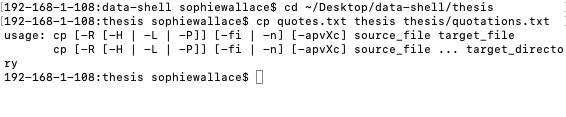
\includegraphics[width=\textwidth]{Images/image1.png}

\subsection{Final Thoughts}
\textbf{6:20PM} Happy I was able to successfully insert the image into the document thanks to a friend. It would be really helpful to work in groups in class to understand errors and reiterate issues. The above image was the result from a previous exercise in Unix shell under "copying files and directories" in journal entry \textit{04/09/2019}. 

\section{05/09/2019}
\subsection{Elaboration Tests}
About to begin testing the tools described in elaboration II to examine whether they meet the specified criteria. Tools include: \textbf{Open Semantic Search} (\textbf{OPSS}), \textbf{Tropy} and \textbf{Excel + Cloudstor Sync Client (CSC).}
\subsection{Intention}
Answer the following questions regarding these tools:
\begin{itemize}
\item Is this tool compatible with all data types?
\item Does this tool organise files with rich metadata?
\item Does this tool allow for editing of data?
\item Can this tool operate offline?
\item Does this tool have a reliable storage system?
\end{itemize}

\subsubsection{Open Semantic Search}
\begin{itemize}
\item \textbf{1:45PM} Downloading OPSS
\item \textbf{2:03PM} Open and Upload OPSS
\item \textbf{2:38PM} Attempting to open OPSS with instructions from Brian and website link
\item \textbf{2:45PM} Open OPSS and begin tests
\end{itemize}


\subsubsection{Tropy}
\begin{itemize}
\item \textbf{2:17PM} Moving onto Tropy tests
\item \textbf{3:12PM} Back onto downloading Tropy whilst I wait for OPSS to download
\item \textbf{3:22PM} Test upload of different data types
\item \textbf{3:32PM} Test organising files and writing rich metadata
\item \textbf{3:38PM} Test viewing and editing data 
\item \textbf{3:41PM} Test operating tropy offline
\item \textbf{3:44PM} Test saving file and storing
\end{itemize}

\subsubsection{DEVONthink 3}
\begin{itemize}
\item \textbf{4:10PM} Downloading Devonthink 3 in an attempt to replace OPSS
\item \textbf{4:20PM} Test if all data types are compatible with application by uploading each
\item \textbf{4:36PM} Test if data can be organised into categories and rich metadata added 
\item \textbf{4:50PM} Test if data can be edited and viewed 
\item \textbf{5:10PM} Test if application can be operated offline
\item \textbf{5:20PM} Test if application can save file and store externally 
\end{itemize}

\subsection{Action}
\subsubsection{Open Semantic Search}
\textit{OSS Download}
\begin{itemize}
\item Entered website
\item Clicked "Download Open Semantic Search"
\item Clicked "Open Semantiic Desktop Search"
\item Clicked hyperlink "Start Virtual Box"
\item Clicked "Download VirtualBox 6.0"
\item Clicked hyperlink "OS X Hosts" platform package 
\item \textbf{SUCCESS} package is downloading onto Mac 
\end{itemize}
\textit{Open and Upload OSS }
\begin{itemize}
\item Dragging VirtualBox item into Applications
\item Double click on VirtualBox from Applications 
\item Pop up box appears "This package will run a program to deteermine if the software can be installed"
\item Click continue
\item Oracle VM VirtualBox for macOS installer appears
\item Click continue
\item "This will take 258.5 MB of space on your computer" 
\item Click continue and proceeds to installation
\item \textbf{ERROR}: System Extention Blocked "A program tried to load new system extensions(s) signed by "Oracle . America,  Inc. if you want to enable these extensions, open Security and Privacy System Preferences" 
\item \textbf{ERROR}: The installation failed. "The Installer encountered an error that caused the installation to fail. Contact manufacturer for assistance"
\end{itemize}

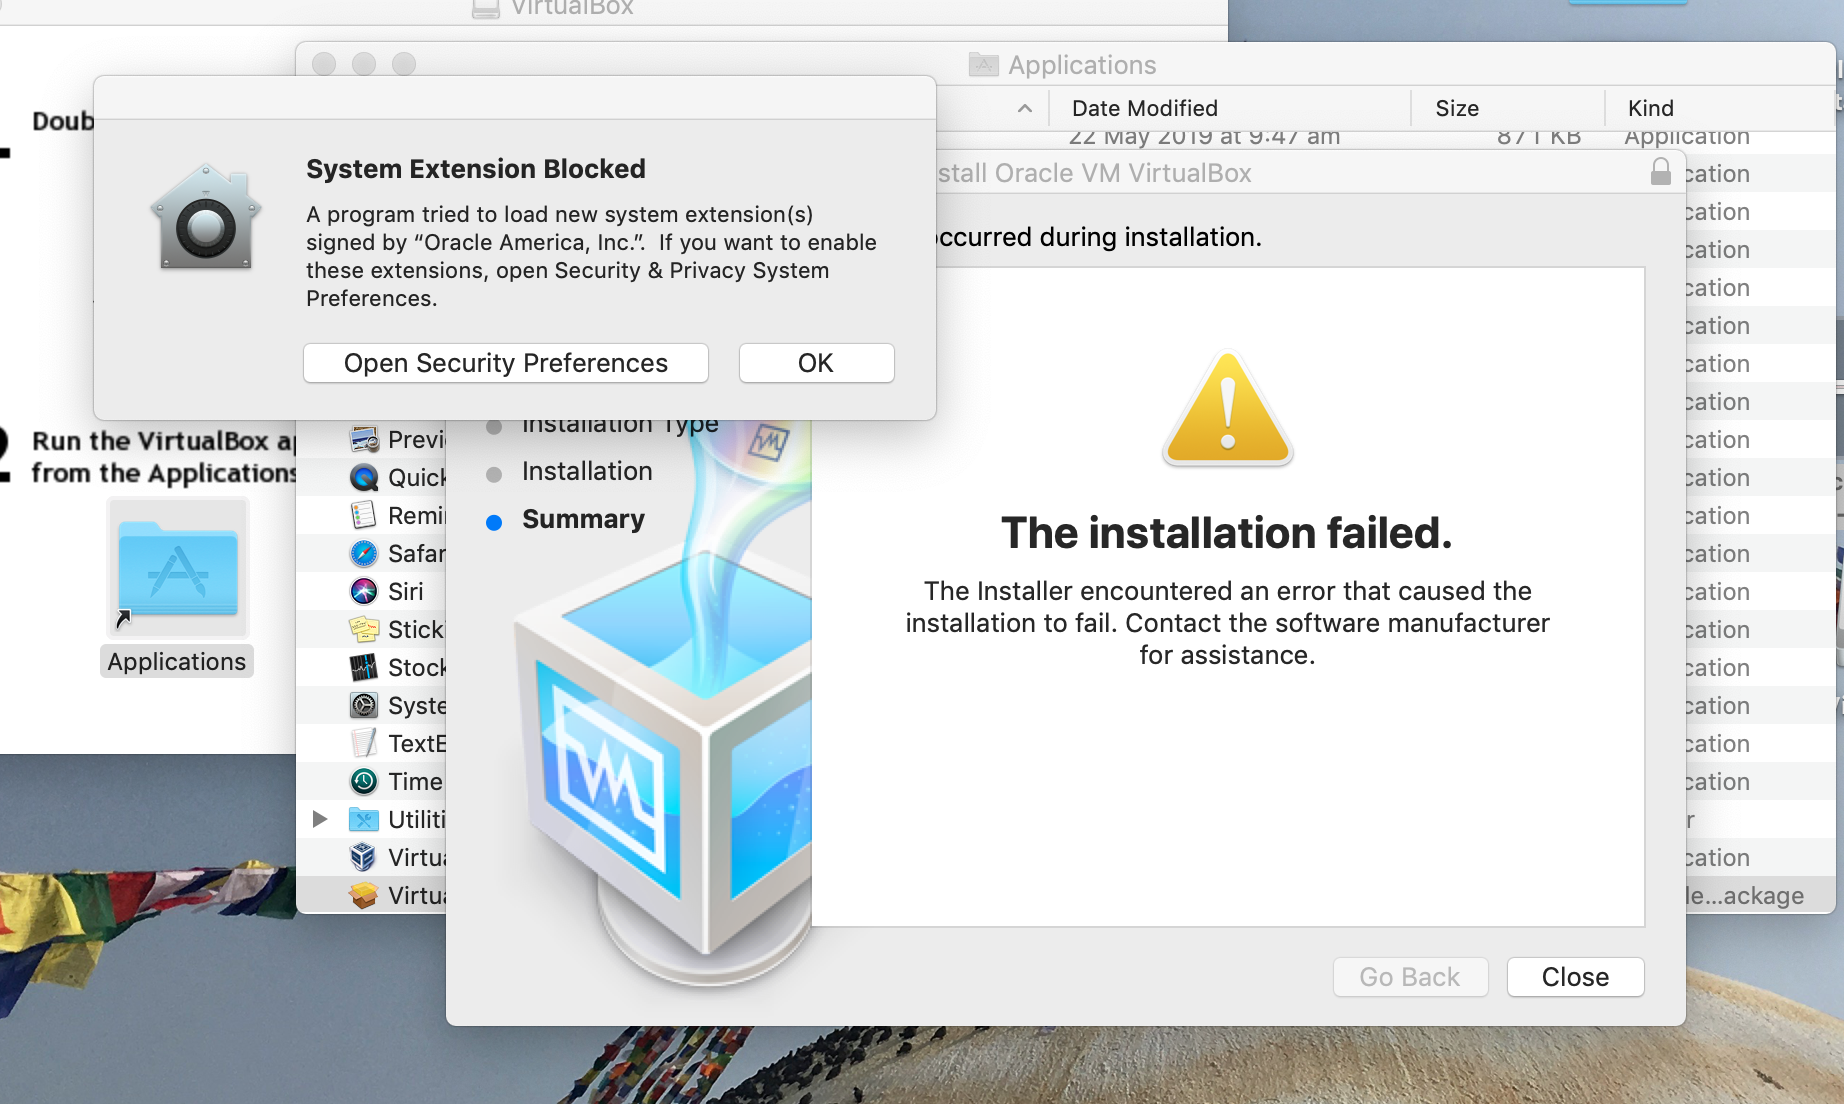
\includegraphics[width=\textwidth]{Images/OSSfail.png}

\textit{Open and Upload OPSS}
\begin{itemize}
\item Clicking through previous steps till I reach error
\item Quit out of the VirtualBox installer after fail
\item Open system preferences on mac
\item Choose "security and Privacy" 
\item Go to "General tab"
\item Click the lock button and enter administrator password
\item Click "allow" at the bottom of the security general section
\item Relaunch VirtualBox Installer (\textbf{SUCCESS})
\item Download the virtual machine image Open Semantic Desktop Search
\item Click on hyperlink "open-semantic-desktop-search19.07.19.ova (3 GB)"under multilingual section on Download page
\item Download is estimated 2 hours
\end{itemize}

\subsubsection{Tropy}
\textit{Download Tropy}
\begin{itemize}
\item Click "Download Tropy for macOS"on Tropy homepage
\item Download estimated for 5 minutes, waiting
\item Dragging Tropy Icon into Applications
\item Double click on Tropy in Applications
\item Window appears "Create a new project"
\item Entering name of project as Elaboration Test and click "create project"
\item \textbf{SUCCESS} Application downloaded and opened onto desktop. Interface displayed below.
\end{itemize}

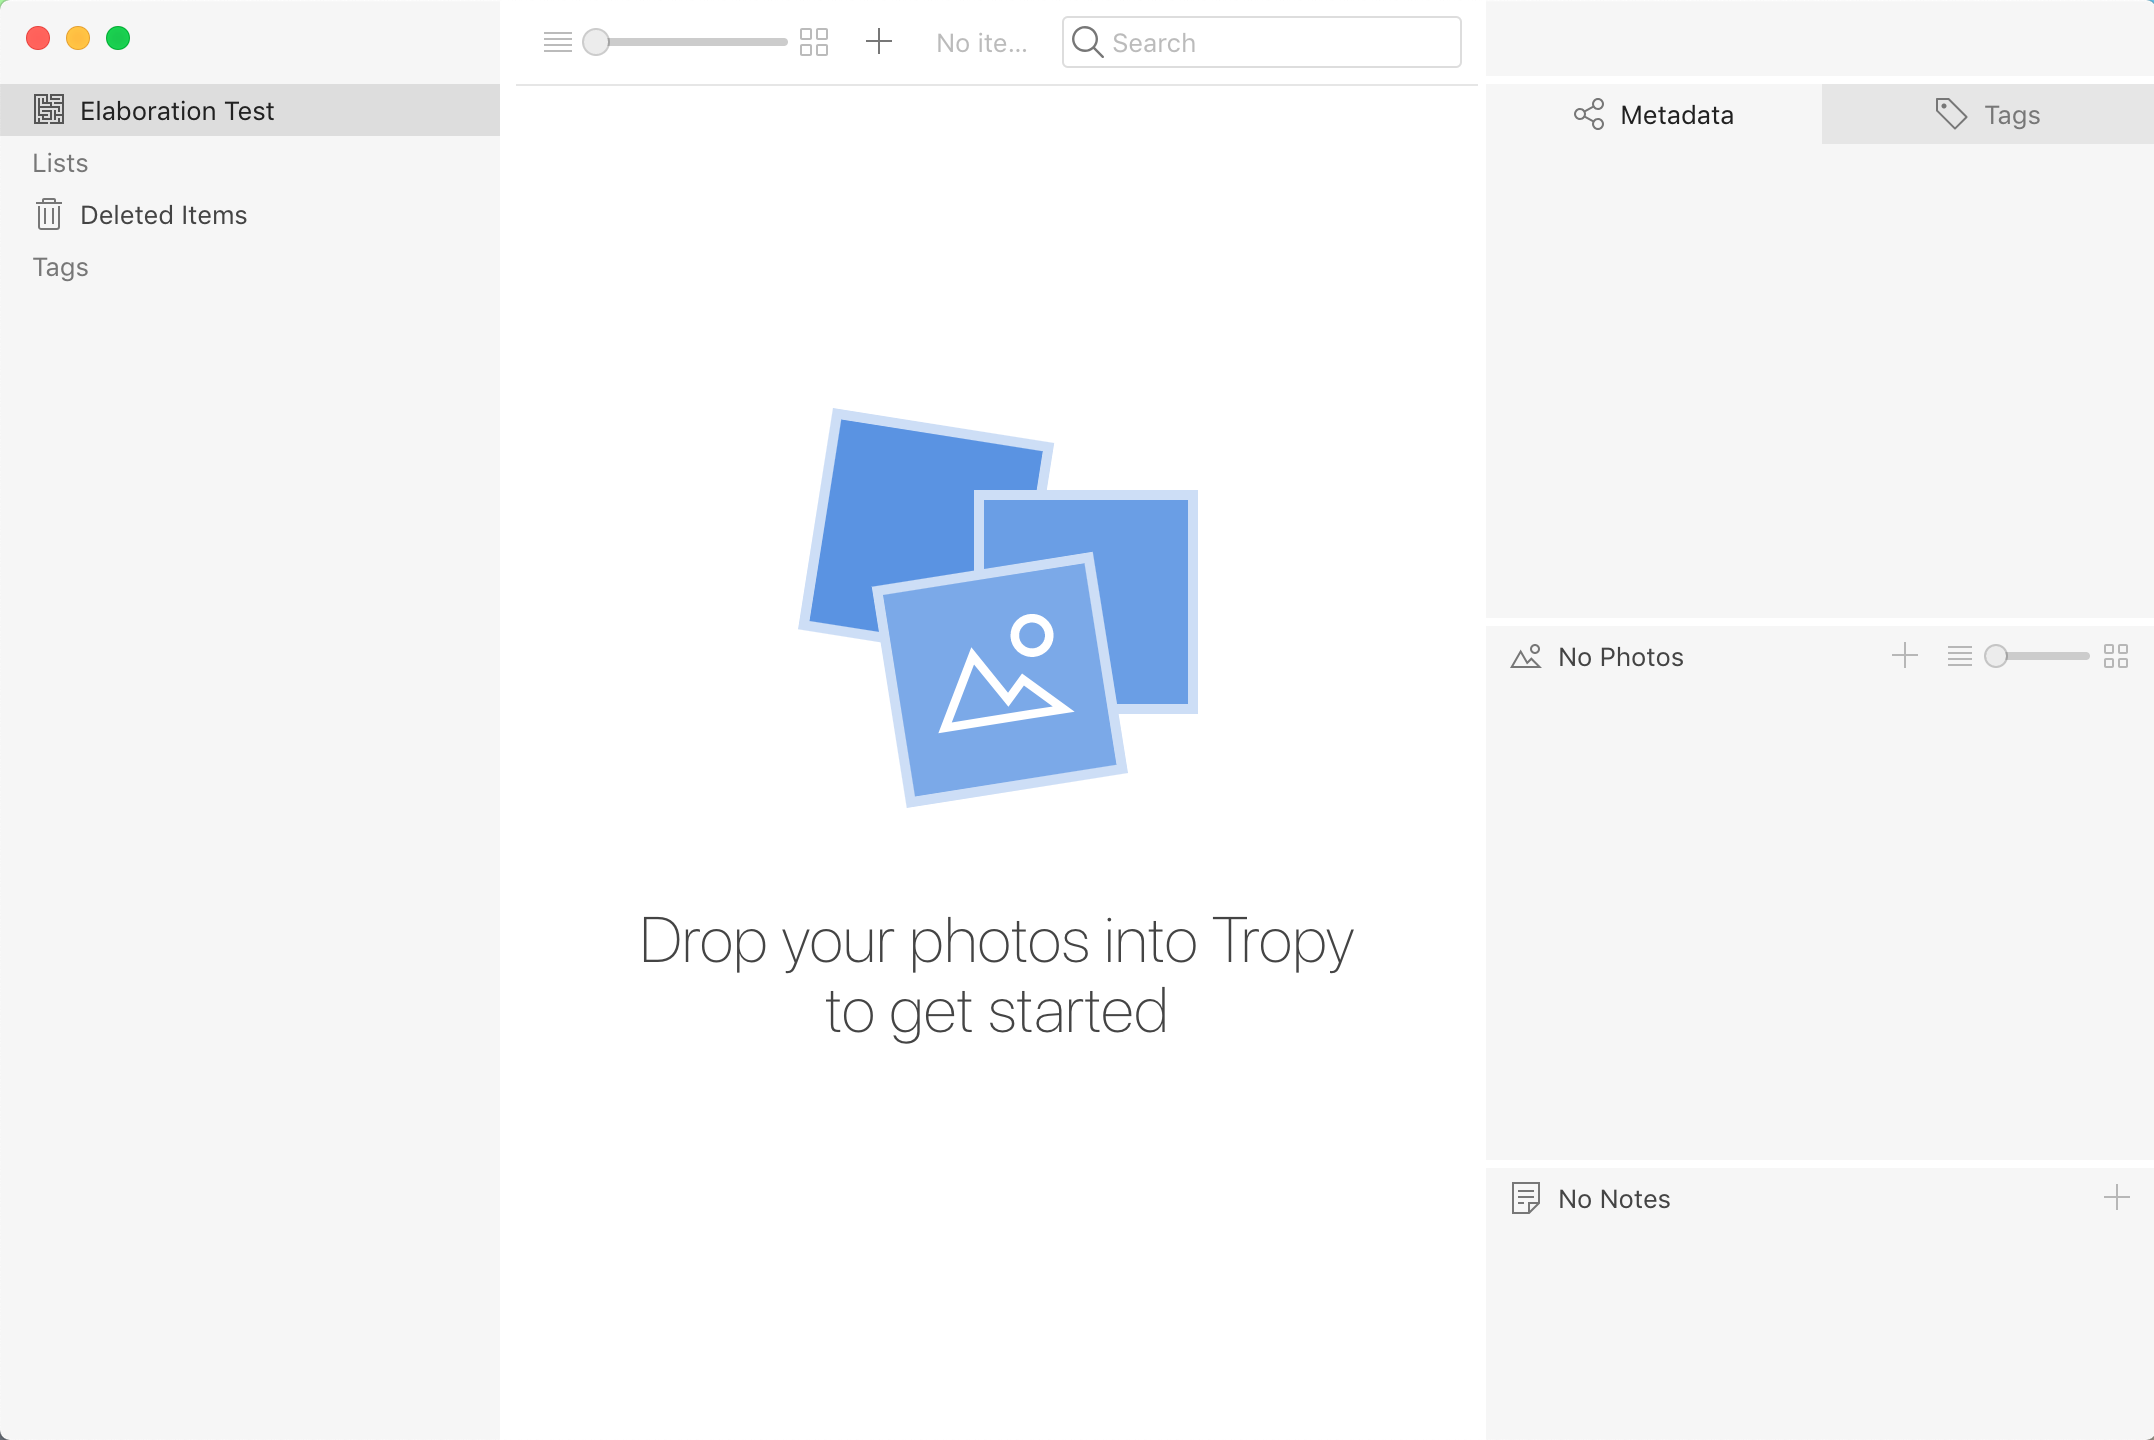
\includegraphics[width=\textwidth]{Images/TropyInterface.png}\\

\textit{Uploading Data Types}
\begin{itemize}
\item Drag photo into Tropy home screen 
\item \textbf{SUCCESS} photo is successfully uploaded
\item Drag text document into Tropy
\item \textbf{ERROR} text document is incompatible
\item Drag audio file into Tropy
\item \textbf{ERROR} audio file is incompatible
\item Drag video file into Tropy
\item \textbf{ERROR} video file is incompatible
\end{itemize}

\textit{Organisation and Writing Rich Metadata}
\begin{itemize}
\item Double click on photograph
\item Opens to a whole metadata section
\item Filling in metadata details
\item \textbf{SUCCESSS} Rich metadata is now included with photo
\item Click on tag function
\item Click Add tag to 1 item
\item Written "elaboration" in tag
\item \textbf{SUCCESS} Tagging feature organises photos into singular or multiple categories
\end{itemize}

\textit{Editing Data}
\begin{itemize}
\item Double clicked on photograph
\item Top right corner has photo adjusting
\item \textbf{SUCCESS} Able to successfully edit minor aesthetics in the photo in the application
\end{itemize}

\textit{Offline Operation}
\begin{itemize}
\item Turning Wifi off
\item Dragging photos from desktop to Tropy
\item \textbf{SUCCESS} Photos can be successfully dropped into Tropy without Wifi
\end{itemize}

\textit{Storage System}
\begin{itemize}
\item Exited Tropy and do not encounter any save option pop ups
\item Searching Tropy interface
\item \textbf{ERROR} No sync or save options
\item Search Tropy website in browser
\item \textbf{SUCCESS} Option to sync Tropy with GitHub
\end{itemize}


\subsubsection{DEVONthink 3}
\textit{Download}
\begin{itemize}
\item Click Download DEVONthink 3 for macOS on home page
\item Drag application icon into the applications folder
\item Double click on DEVONthink 3 in application folder
\item \textbf{SUCCESS} Application is now opened and running on my desktop (Screenshot below displays home screen interface)
\end{itemize}

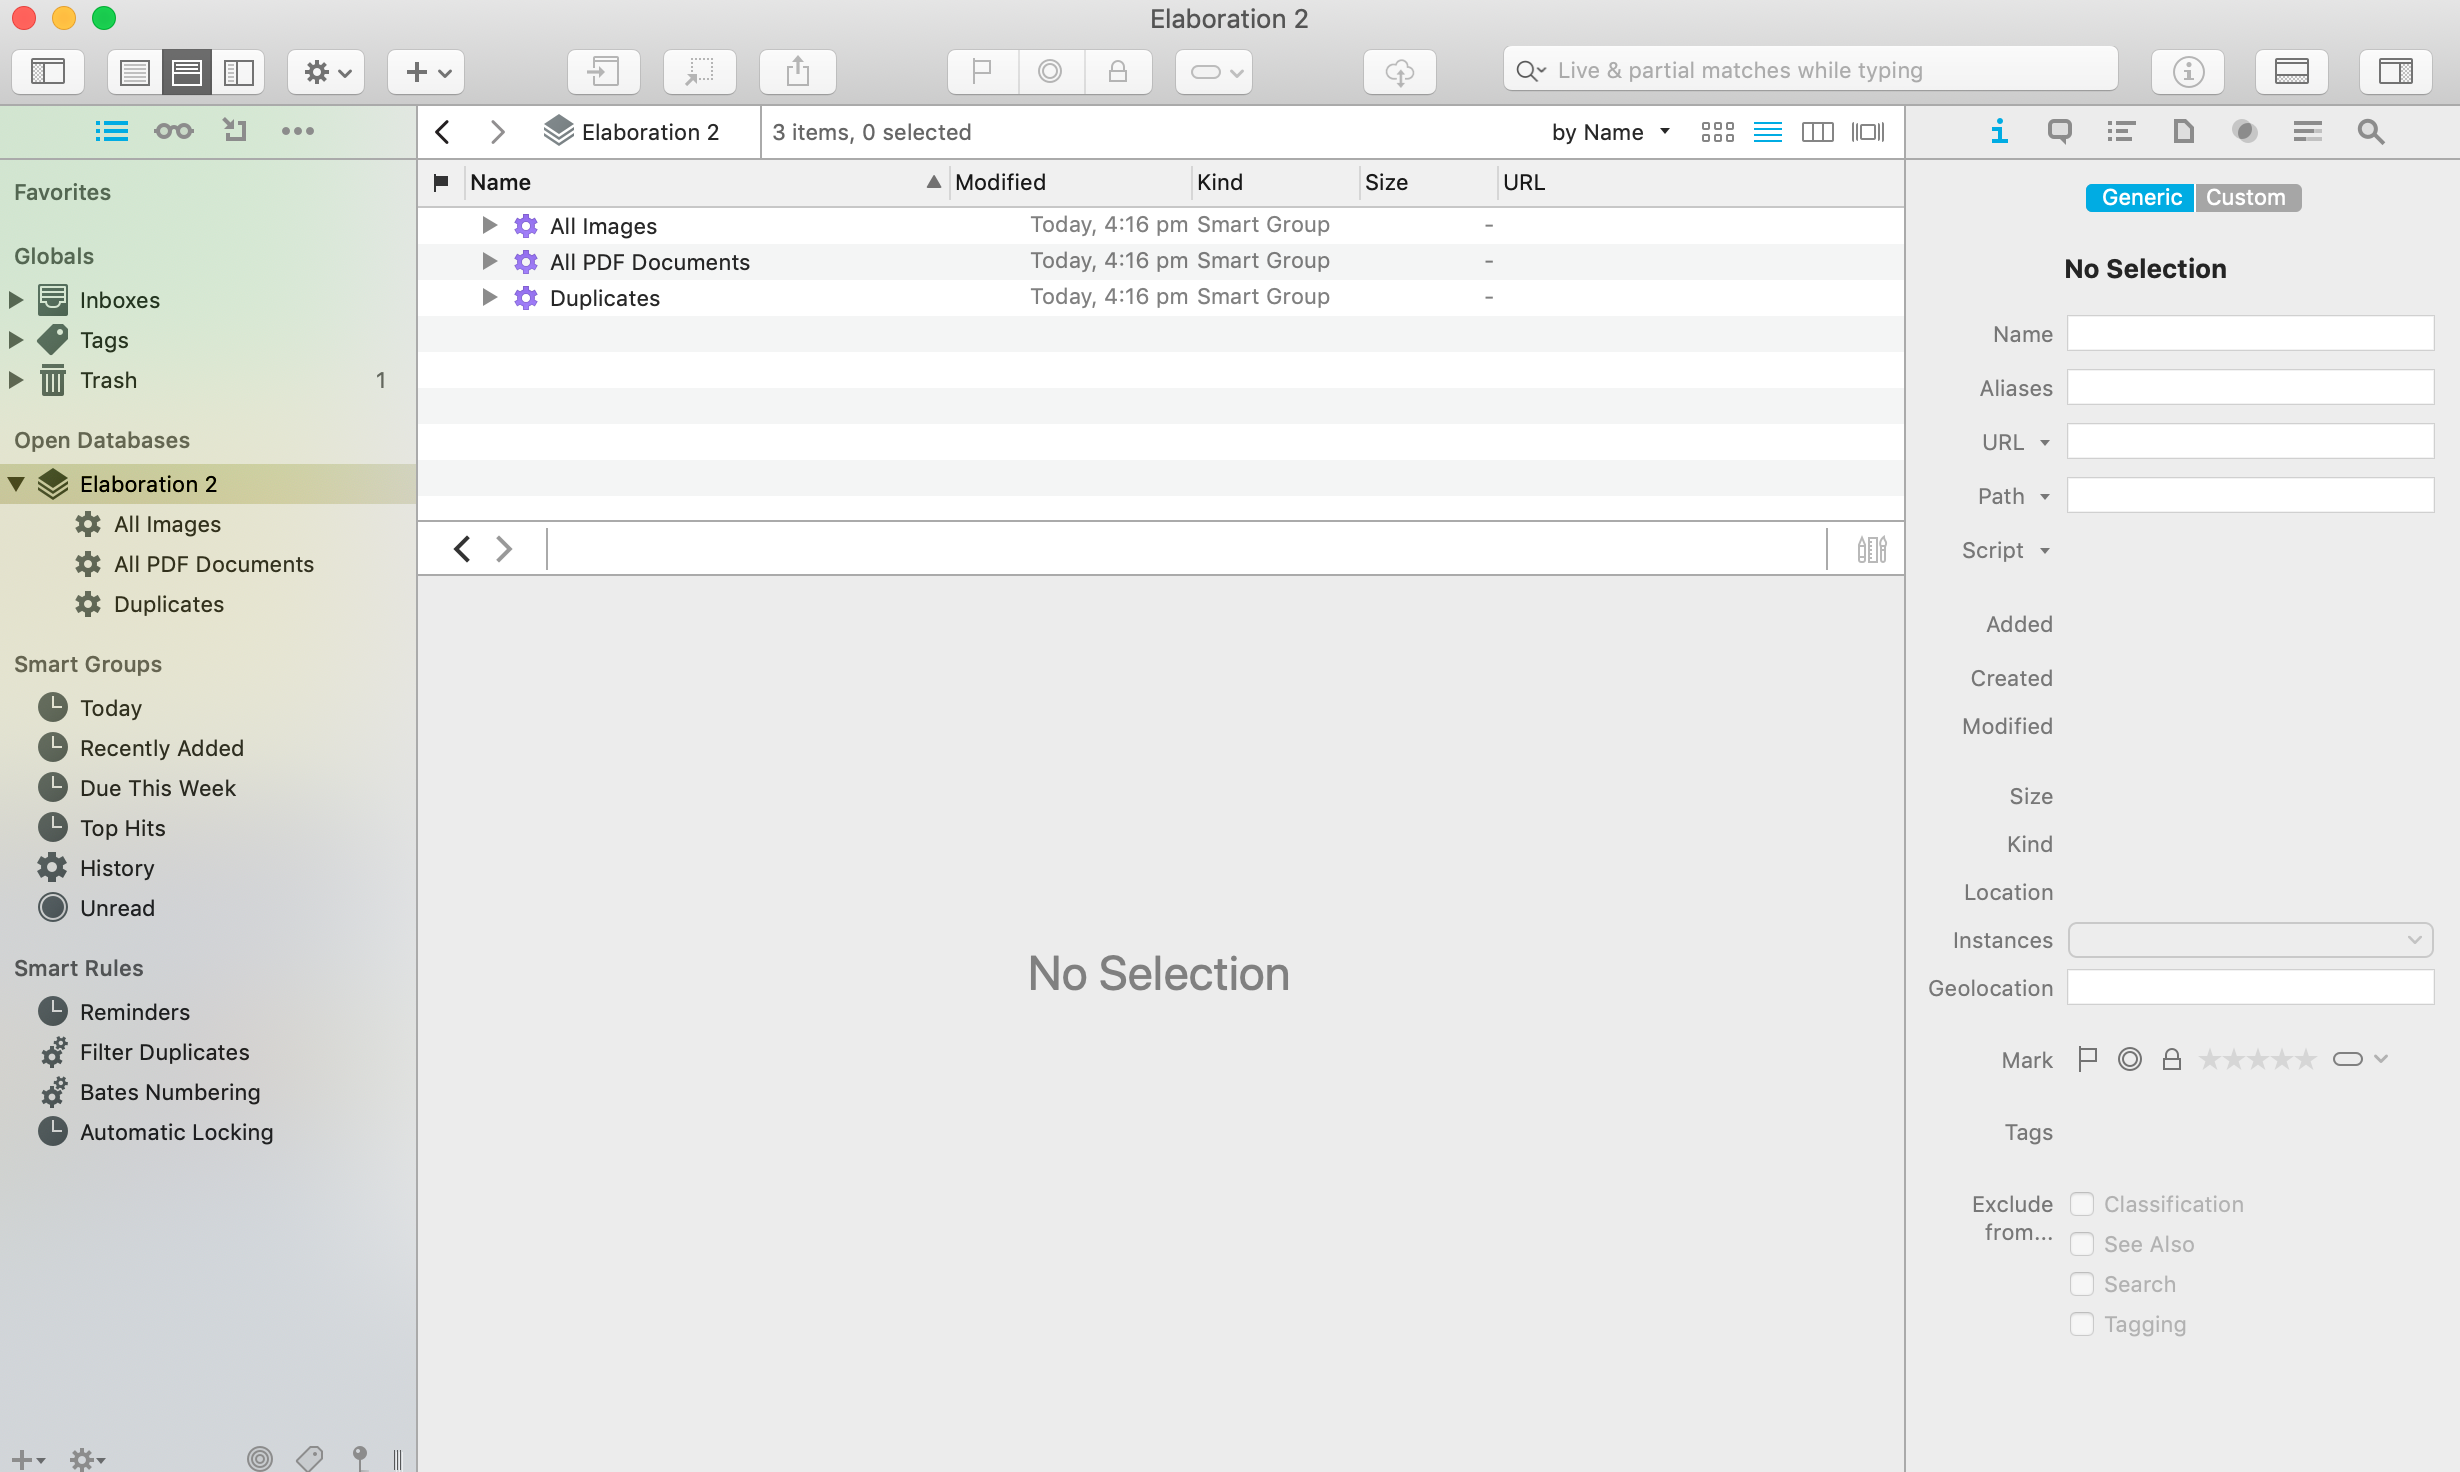
\includegraphics[width=\textwidth]{Images/DEVONinterface.png}

\textit{Uploading Data Types}
\begin{itemize}
\item Clicked create new database in file and named "Elaboration 2"
\item Dragging image into application
\item \textbf{SUCCESS} Image is uploaded successfully into application
\item Dragging text document into application
\item \textbf{SUCCESS} Text file is uploaded successfully into application
\item Dragging audio file into application
\item \textbf{SUCCESS} Audio file is uploaded successfully into application
\item Dragging video file into application
\item \textbf{SUCCESS} Video file is uploaded successfully into application
\end{itemize}

\textit{Organising and Writing Rich Metadata}
\begin{itemize}
\item Clicked on audio file
\item Right column opens allowing for information on data type
\item Writing name for audio file
\item Writing notes in comment section
\item Added tag for categorization
\item \textbf{SUCCESS} Organised into a category and metadata has been added
\end{itemize}

\textit{Editing Data}
\begin{itemize}
\item Clicking on text document 
\item Double clicking opens document on desktop in its own application
\item Exiting word
\item Single click on text document
\item Text document below
\item \textbf{SUCCESS} text is able to be edited in application
\end{itemize}

\textit{Operating Offline}
\begin{itemize}
\item Turning wifi connection off
\item \textbf{SUCCESS} Application is able to be upload and edit whilst offline.
\end{itemize}

\textit{Saving and Storage}
\begin{itemize}
\item Click preferences
\item Click sync tab
\item \textbf{SUCCESS} Multiple sync locations are already inbuilt and additional sync options can be added
\end{itemize}


\subsection{Final Thoughts}
\subsubsection{Open Semantic Search}
\textbf{2:10PM} I'm unsure about this download and don't want to get a virus or change my settings without being certain. I will share this journal with Brian to ask what he thinks. Excited I included the screenshot without needing to refer to prior notes though. \\
\textbf{3:02PM} Realised I had only downloaded VirtualBox, just one component of this software package. With download time estimated at 2 hours I will move back to Tropy. \\
\textbf{4:08} Estimated time for OPSS has not gone down. I have found another technology I would like to try instead so I am removing OPSS from this elaboration at the time being. 

\subsubsection{Tropy}
\textbf{3:31PM} Uploading Data Types: Photos are uploaded with ease in a swift dragging motion, however all other data types are incompatible. \\
\textbf{4:02PM} Tropy has a lot of pain relievers and gain creators when it comes to my POC. It operates offline, organises and writes rich metadata, has inbuilt editing functions for photos, and has an easy to use interface that is also aesthetically pleasing. However, Tropy is specifically for photo management and does not cater to all kinds of data types. 

\subsubsection{DEVONthink 3}
\textbf{5:44PM} DEVONthink 3 has a lot of great features that meet the specified criteria. Many pains are addressed and its function has numerous gain creators. The fact that it is compatible with all data types, syncs to an online storage, allows editing of text and provides rich metadata is fantastic. It also has gains that were not specified such as in-built add-ons. These extensions are installed onto a browser so you can easily store additional data from the internet such as websites and references. The interface for this tool is not that appealing and needs further work, I would prefer something that has less clutter and features on the initial home page, however you are able to customize the layout so further interaction with the technology may solve this. Also, to gain access to the full features of this tool the user must pay an additional fee. Similarly if you want to download the mobile application, it costs. 

\section{06/09/2019}
\subsection{Elaboration Tests}
Continuing on with elaboration tests for excel + cloudstor sync client (CSC).
\subsection{Intention}
Answer the following questions regarding this tool:
\begin{itemize}
\item Is this tool compatible with all data types?
\item Does this tool organise files with rich metadata
\item Does this tool allow for editing of data?
\item Can this tool operate offline?
\item Does this tool have a reliable storage system?
\end{itemize}

\subsubsection{Excel + CSC}
\begin{itemize}
\item \textbf{10:09AM} Test if this tool is compatible with all data types?
\item \textbf{10:24AM} Test is this tool can organise . files with rich metadata
\item \textbf{10:29AM} Test if this tool allows for editing data
\item \textbf{10:35AM} Test if this tool can operate offline
\item \textbf{10:40AM} Test if this tool can sync onto storage system
\end{itemize}



\subsection{Action}
\subsubsection{Excel + CSC}
Uploading Data Types
\begin{itemize}
\item Open Excel
\item Click create new work book
\item Drag image into excel
\item \textbf{SUCCESS} Image can be uploaded into application
\item Drag audio file into excel
\item \textbf{SUCCESS} audio file can be uploaded into application
\item Drag word document into excel
\item \textbf{ERROR} Word document is unable to be uploaded
\item Drag video file into excel
\item \textbf{SUCCESS} video file can be uploaded into application
\end{itemize}
Management and Metadata
\begin{itemize}
\item Click on image file and move into excel box
\item \textbf{ERROR} Image does not automatically go into box
\item Write categories of data in excel
\item \textbf{SUCCESS} Categories for type file can be entered
\item Write descriptions of data in excel
\item \textbf{SUCCESS} Descriptions able to be included
\end{itemize}
Editing Data
\begin{itemize}
\item Double click on image
\item \textbf{SUCCESS} Editing tab appears
\item Double click on video file
\item \textbf{ERROR} Video file plays and no editing tab appears
\item \textbf{ERROR} Excel crashes expectantly
\item \textbf{ERROR} Pop up appears "Microsoft Excel has crashed expectantly. Sorry for the inconvenience. We are trying to recover your work now."
\item \textbf{ERROR} Video has disappeared
\item Double click on Audio file
\item Sound from file plays
\item Click escape for sound to stop playing
\item \textbf{ERROR} No editing tab appears
\end{itemize}
Offline Operation
\begin{itemize}
\item Turn wifi off 
\item Drag image file into Excel 
\item Write metadata in cell
\item \textbf{SUCCESS} Image is uploaded and metadata is written
\end{itemize}
Saving and Storage 
\begin{itemize}
\item Visit cloudstor sync client website
\item Click download desktop sync client 
\item Open cloustor client installer
\item Click continue in CSC installer
\item "This will take 97.6 MB of space on your computer"
\item Click install
\item \textbf{SUCCESS} Installation was successful
\item Double click on cloudstor application
\item Enter user credentials 
\item \textbf{ERROR} "Access forbidden by server. To verify that you have proper access, click here"
\item Click on hyper link 
\item \textbf{ERROR} Entered cloudstor with studentID and changed password, no luck with CSC
\item Click on hyperlin on CSC window to "request an app password from the web interface.
\item Type in app name to create new app password
\item Type in CloudStor Client
\item Recieved password/token
\item Copy password into app
\item \textbf{ERROR} Access forbidden by server. To verify that you have proper access, click here to access the service with your browser.
\item Trying that hyper link one more time
\item Sends me to my cloudstor homepage with no additional prompts
\item Attempt to just press next again with credentials entered
\item \textbf{SUCCESS} connects me into setting up local folder options (out of nowhere)
\item Option to synchronise all (Recommended)
\item Click sync all
\item Paused sync process as I want to only see if it works for Excel
\item Click save as for workbook
\item Select save in cloudstor folder
\item Open cloudstor browser
\item \textbf{ERROR} File does not appear in cloudstor browser
\end{itemize}


\subsection{Final Thoughts}
\textbf{11:05AM} Utilizing excel with the CSC proved to be more challenging than anticipated. Although most data types can be included, they are not managed or organized automatically. Whilst metadata could be rich in detail if manually entered, the technical debt acquired from this process would be extensive. The test for CSC was inconclusive as the file saving process was unclear. This may have been due to pausing synchronisation due to not wanting 13GB loaded onto my small memory disk. Excel would work better for manually entering only metadata rather than managing different data files.

\section{07/09/2019}
\subsection{Thoughts/Intentions}
\textbf{12:08PM} Attempting remaining Unix shell exercises

\subsection{Action}
Pipes and Filters
\begin{itemize}
\item Command: ls molecules
\item \textbf{ERROR} No such file or directory
\item Command pwd: find current working directory
\item Location /Users/sophiewallace
\item Command ls: listing contents in directory
\item Command cd /Users/sophiewallace/Desktop/data-shell
\item \textbf{SUCCESS} located myself into data-shell directory
\item Command ls molecules: Listing contents
\item Command cd molecules
\item Command wc *.pbd: \textbf{SUCCESS}listed word count 
\item Command wc -l 
\item \textbf{ERROR} lost dollar command sign
\item Command cntrl + c:  \textbf{SUCCESS} regained command sign
\item Command cat lengths.txt
\item Command wc -l *.pbd > lengths.txt 
\item \textbf{ERROR} No such file or directory
\item Command echo hello > testfile.01.txt
\item \textbf{ERROOR} No response
\item Command data-shell/data/animals.txt
\item \textbf{ERROR} No such file or directory exists
\item Command sort -n lengths.txt | head -n 1
\item \textbf{ERROR} No Response from commands
\item Command wc -l *.pdb | sort -n | head -n 1
\item \textbf{SUCCESS} pipe led me to methane.pdb
\end{itemize}
Loops
\begin{itemize}
\item Command l: refreshing lines in terminal
\item \textbf{SUCCESS} refreshed terminal
\item Command cd /Users/sophiewallace/Desktop/data-shell/creatures
\item \textbf{SUCCESS} Located in creatures directory
\item Command head -n 5 basilisk.dat minotaur.dat unicorn.dat
\item \textbf{SUCCESS} Displaying structures of files
\item Command for filenes in *.dat
\item Command > do
\item Command >  echo (dollarsign)filename
\item Command >  head -n 100 (dollarsign)filename | tail -n 20
\item Command > done
\item Command cntrl + c
\item \textbf{SUCCESS} regained dollar sign command
\item Command (dollarsign) for filename in *.dat
\item Command > do
\item Command >     cp (dollarsign)filename original-(dollarsign)filename
\item Command > done
\item \textbf{SUCCESS} 
\end{itemize}
Shell Scripts
\begin{itemize}
\item Command cd /Users/sophiewallace/Desktop/data-shell/molecules
\item \textbf{SUCCESS} In molecule file
\item Command nano middle.sh
\item \textbf{SUCCESS} text editor opened
\item Written in text editor "head -n 15 octane.pdb | tail -n 5"
\item Command cntrl-0 \textbf{SUCCESS} file saved
\item Command cntrl-c \textbf{SUCCESS} exited nano
\item Look in molecules folder 
\item \textbf{SUCCESS} file is created
\item Command bash middle.sh
\item \textbf{SUCCESS} Script displays output for pipeline
\item Command nano middle.sh
\item Replacing octane.pdb to dollarsign 1
\item \textbf{ERROR} frozen terminal functions and "1" is infront of head
\item Command cntrl x to exit and N for no saving
\item Command nano middle.sh
\item Move through text with arrows
\item Replace octane.pdb to dollarsign 1
\item Save and exit command
\item Command bash middle.sh octane.pdb
\item \textbf{SUCCESS} Script displays output for pipeline
\item Command nano middle.sh
\item Replace text with head -n "(dollarsign)2" "(dollarsign)1" | tail -n "(dollarsign)3"
\item Save and exit
\item Command bash middle.sh pentane.pdb 15 5
\item Command bash middle.sh pentane.pdb 20 5
\item \textbf{SUCCESS} Changed scripts behaviour
\item Command nano middle.sh
\item Add comments above script
\item Select lines from the middle of a file.
\item Usage: bash middle.sh filename end(underscore)line num(underscore)lines
\item Save and exit nano
\item Command nano sorted.sh
\item Insert command lines from Unix
\item Save and exit
\item Command bash sorted.sh *.pdb ../creatures/*.dat
\item \textbf{SUCCESS} Sorted list of other kinds of files
\end{itemize}
Finding Things 
\begin{itemize}
\item Command cd Desktop/data-shell/writing
\item Command cat haiku.txt
\item \textbf{SUCCESS} Located haiku subdirectory
\item Command  grep not haiku.txt
\item \textbf{SUCCESS} Located lines that contain the word not
\item Command grep The haiku.txt
\item \textbf{SUCCESS} Located lines containing the word the
\item Command grep -w The haiku.txt
\item \textbf{SUCCESS} limits matches to word boundaries
\item Command grep -w "is not" haiku.txt
\item \textbf{SUCCESS} Phrase containing is not found
\item Command grep -n "it" haiku.txt
\item \textbf{SUCCESS} Useful to use quotes when searching for multiple words
\item Command grep -n -w "the" haiku.txt
\item \textbf{SUCCESS} Combined options (i.e. flags) as we do with other Unix commands
\item Command grep -n -w -i "the" haiku.txt
\item \textbf{SUCCESS} Search is now case-insensitive
\item Command grep -n -w -v "the" haiku.txt
\item \textbf{SUCCESS} Search is now inverted
\item Command grep --help
\item \textbf{SUCCESS} and \textbf{ERROR} Options appear but they are not presented as Unix Shell, more haphazard and hard to read. \\

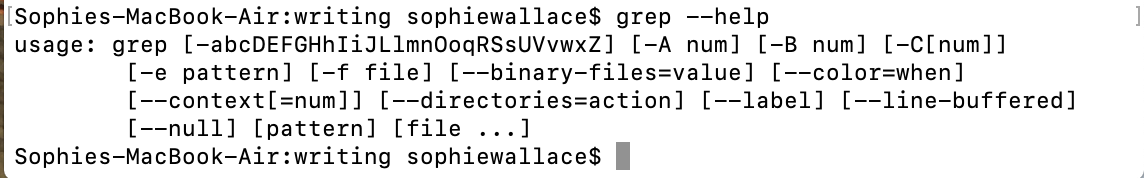
\includegraphics[width=\textwidth]{Images/grep--help.png} \\
\item Command find . -type d
\item \textbf{SUCCESS} Name of 5 directories appear
\item Command find . -type f
\item \textbf{SUCCESS} Name of files appear 
\item Command find . -name *.txt
\item \textbf{SUCCESS} Name matched
\item Command  find . -name '*.txt'
\item \textbf{SUCCESS} Expanded file name appears
\item Command wc -l dollarsign(find . -name '*.txt')
\item \textbf{SUCCESS} Find command utilised inside brackets
\end{itemize}

\subsection{Key Points}
Pipes and Fliter Key Points \\
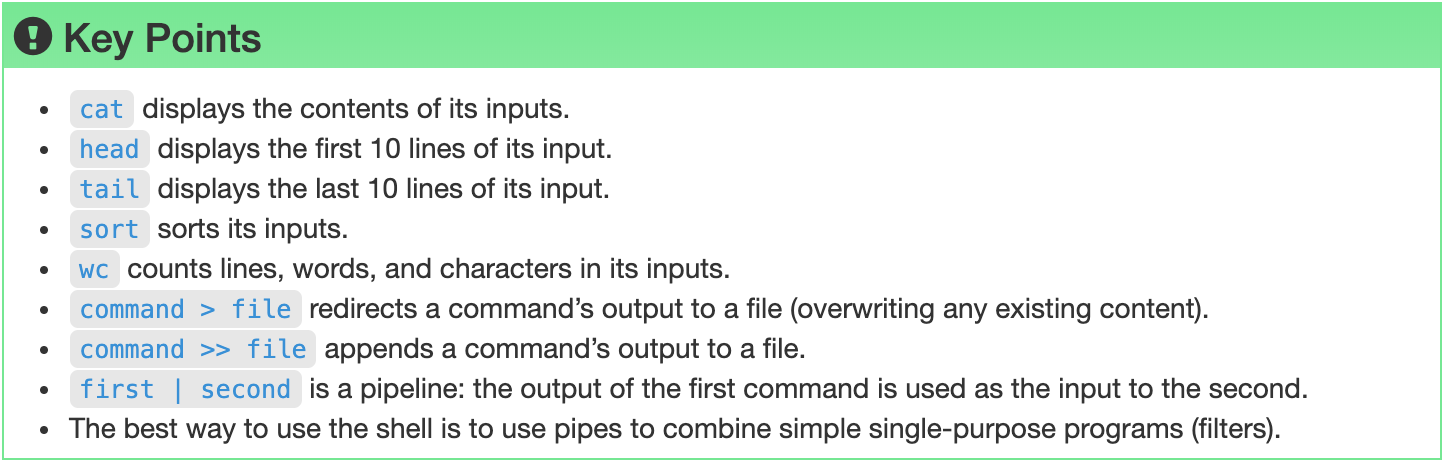
\includegraphics[width=\textwidth]{Images/PipesFilters_KP.png}\\
Loops \\
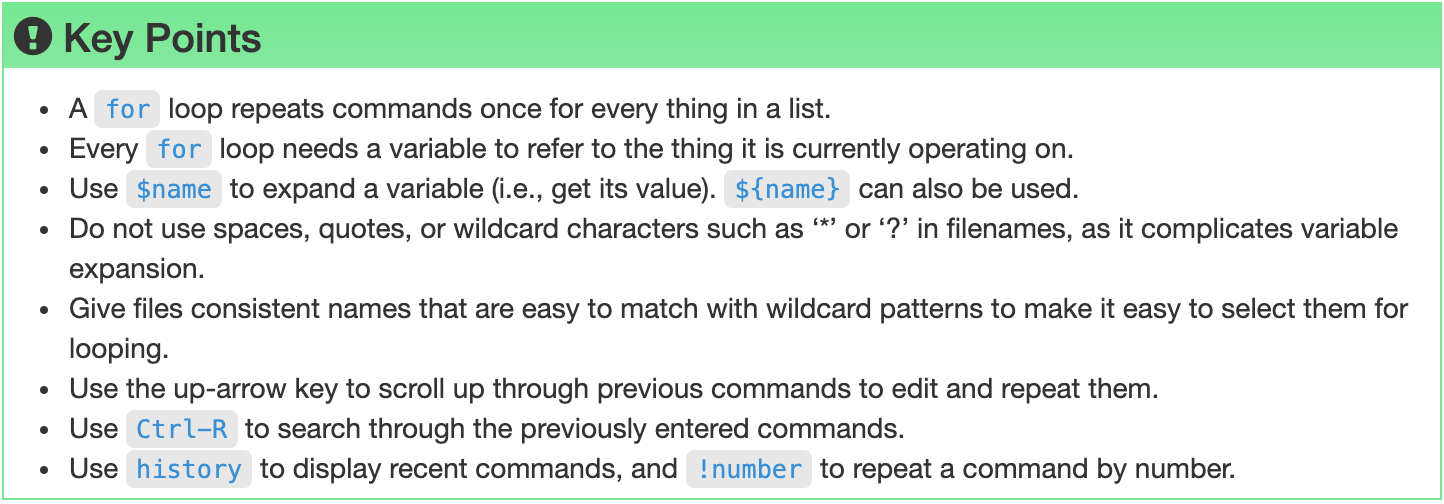
\includegraphics[width=\textwidth]{Images/Loop_KP.png} \\
Writing Shell Scripts \\
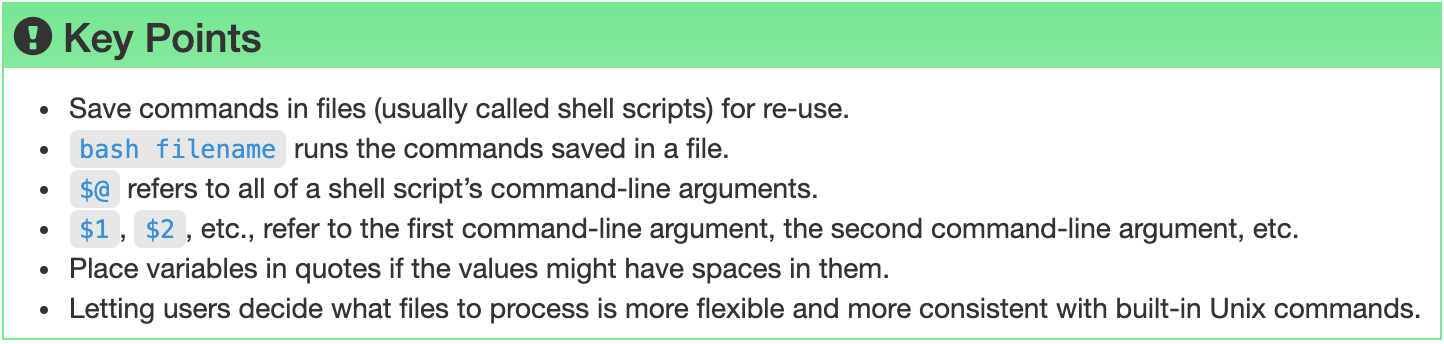
\includegraphics[width=\textwidth]{Images/WritingShellScripts_KP.png} \\
Finding Things \\
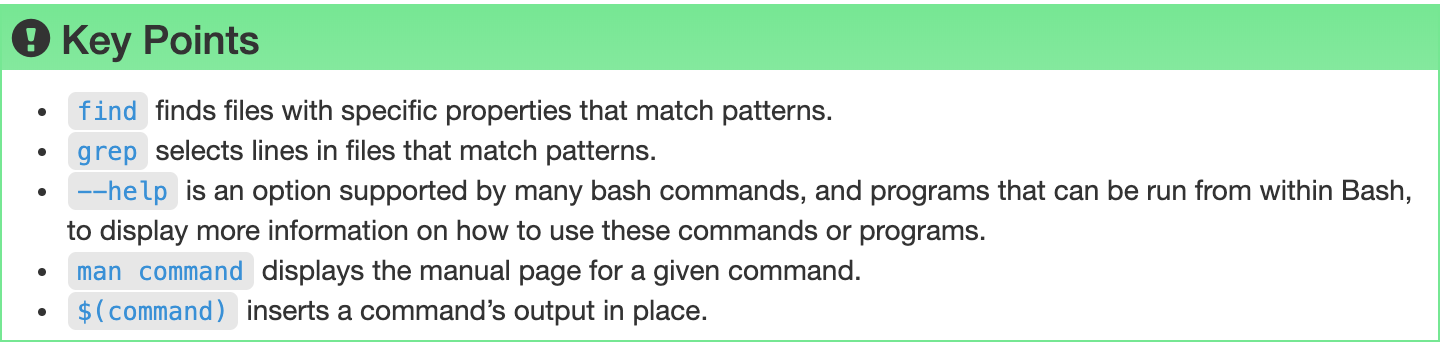
\includegraphics[width=\textwidth]{Images/FindingThings_KP.png} \\

\subsection{Final Thoughts}
\textbf{1:45PM} I found these shell exercises interesting, especially writing shell scripts and finding things. The loop section was difficult and used many commands that were not in a familiar order so I would need more practice in looping. Adding screen shot of the key points helps to display the commands without encountering an error in overleaf. I like how much I've learnt with overleaf in the past week, however terminal is still rather illusive to me. 

\section{09/09/2019}
\subsection{Thoughts/Intentions}
Interested in adding more formatting in overleaf to professionalize documents. \\
\textbf{7:28PM} Adding hyperlinks to the table of contents \\
\textbf{7:33PM} Adding figures/captions to photos\\
\textbf{7:50PM} Add secondary figure to see result\\

\subsection{Action}
Hyperlink
\begin{itemize}
\item Added usepackage hyperref in the preamble
\item Recompiled document
\item \textbf{SUCCESS} Hyperlinks in table of contents created.
\end{itemize}
Photo Captions
\begin{itemize}
\item Utilizing commands in photo inserted below
\end{itemize}
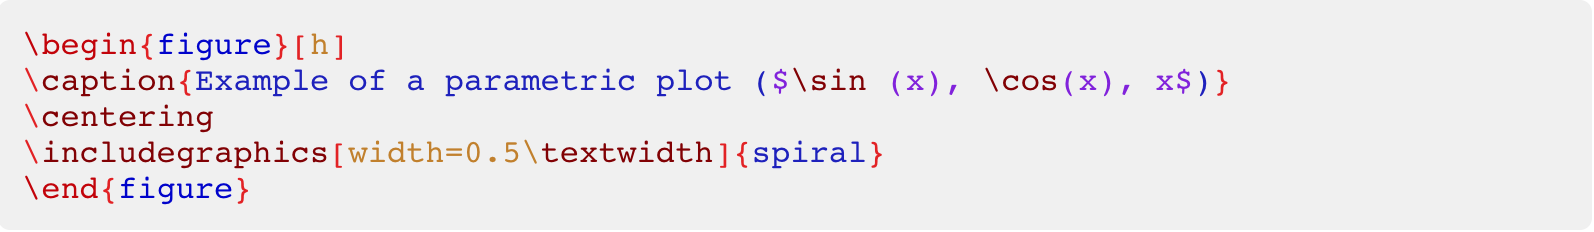
\includegraphics[width=\textwidth]{Images/CaptionTest.png}\\
\begin{itemize}
\item \textbf{SUCCESS} Photo was included however formatting is off 
\item Add text width in include graphics command
\item \textbf{SUCCESS} Photo is displayed below in Figure 1: Caption Test.
\end{itemize}
\begin{figure}[H]
    \centering
    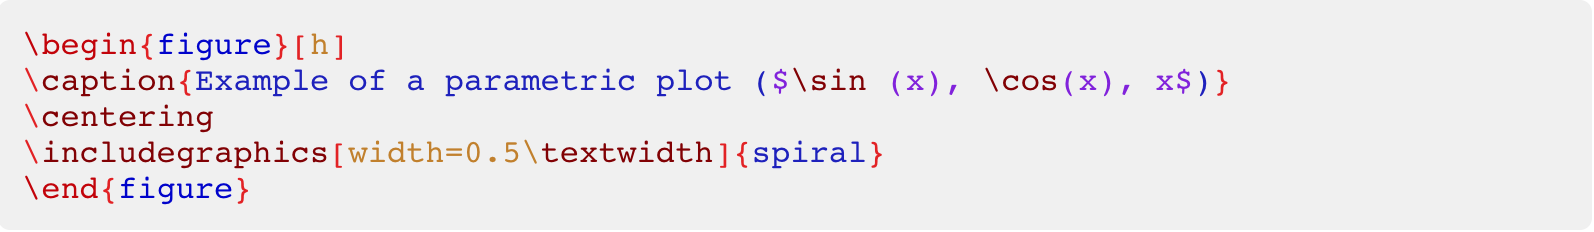
\includegraphics[width=\textwidth]{Images/CaptionTest.png}
    \caption{Caption Test}
    \label{fig:my_label}
\end{figure} 

Second Figure 
\begin{figure}[H]
    \centering
    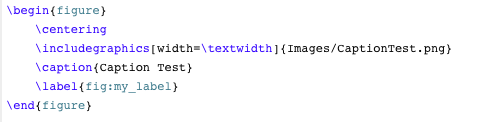
\includegraphics[width=\textwidth]{Images/CaptionTest2.png}
    \caption{Caption}
    \label{fig:my_label}
\end{figure}
\begin{itemize}
\item Enter figure command with image
\item \textbf{SUCCESS} Figure enters as Figure 2. Yet formatting is off and images appear irrelevant of text/line order
\item Add float package and H parameter to figure 
\item \textbf{SUCCESS} Figures are now aligned as written in LaTeX code
\end{itemize}

\subsection{Final Thoughts}
\textbf{8:05PM} I really enjoy using LaTeX and have found it interesting to play around with. I like that I have been able to add captions to the images, which was bugging me when formatting during Elaboration. Also glad hyperlinks in the table of contents are now added for easier reference.

\section{16/09/2019}
\subsection{Thoughts/Intentions}
\textbf{2:17PM}: Beginning open refine data carpentry exercises. \\
\textbf{4:04PM}: Beginning Filtering and Sorting with OpenRefine

\subsection{Action}
Working with OpenRefine
\begin{itemize}
\item Click create project
\item Select get data from this computer
\item Click choose files
\item select SAFI OpenRefine 
\item Click open
\item Click Next 
\item Click update preview
\item Click create project
\item \textbf{SUCCESS} SAFI OpenRefine is uploaded \\
\end{itemize}
Using Facets
\begin{itemize}
\item Scroll to village column
\item Click down arrow and choose Facet then Text Facet
\item Click sort by name/count to view different presentations of data
\item Click interview date column
\item Click down arrow and choose Facet>text facet
\item \textbf{SUCCESS} There are 19 choice for interview dates
\item Click edit next to interview date
\item \textbf{SUCCESS} Column is formatted in text
\item Click down arror and choose Edit cells>common transforms then to date
\item \textbf{SUCCESS} Column has been converted to dates
\item Scroll through dates in column
\item Data was mainly collected in Nov 2016
\end{itemize}
Clustering
\begin{itemize}
\item Click cluster button in village text facet
\item Click through method and keying functions for alternate displays
\item Select key collision methods and metaphone3 key function
\item \textbf{SUCCESS or ERROR} 6 Clusters were identified, not 2
\item Click merge for first cluster Ruaca and Ruca
\item Click merge selected and recluster
\item Click merge for second cluster Ruaca-Nhameuenda to Ruaca - Nhamuenda
\item Click merge selected and recluster
\item \textbf{SUCCESS} There are now no clusters
\item Exit Cluster pop up
\item Click edit Chirdozo then change name to Chirodzo
\item \textbf{SUCCESS} Data has merged
\item Repeat with Ruaca-Nhamenda
\item \textbf{SUCCESS} Data has merged and only 4 clusters remain
\end{itemize}
Transforming Data
\begin{itemize}
\item Click down arrow in items owned column
\item Choose edit cells then transform...
\item \textbf{SUCCESS} GREL expression popup opened
\item Removing left square brackets typing value.replace("[", "") in box
\item Click OK
\item \textbf{SUCCESS} All left square brackets gone
\item Click down arrow 
\item Choose edit cells then transform
\item Type value.replace("'", "") to remove single quote mark
\item \textbf{SUCCESS} single quote mark removed from column
\item Click down arrow 
\item Choose edit cells then transform
\item Type value.replace("]", "") to remove right square bracket
\item \textbf{SUCCESS} right square bracket removed from column
\item Click down arrow 
\item Choose edit cells then transform
\item Type value.replace(" ", "") to remove spaces from column
\item \textbf{SUCCESS} spaces removed from column and items separated by semicolons
\item Click down arrow
\item Choose facet then custom text facet..
\item Type value.split(";") in expression box
\item click ok
\item \textbf{SUCCESS} New text facet box 
\item Click count to see common items
\item Click down arrow on months lack food
\item Choose edit cells then transform
\item Type value.replace("]", "") to remove right square bracket
\item click ok
\item \textbf{SUCCESS} right square bracket removed from column
\item Click down arrow 
\item Choose edit cells then transform
\item Type value.replace("'", "") to remove single quote mark
\item \textbf{SUCCESS} single quote mark removed from column
\item Click down arrow 
\item Choose edit cells then transform
\item Type value.replace("]", "") to remove right square bracket
\item \textbf{SUCCESS} right square bracket removed from column
\item Click down arrow 
\item Choose edit cells then transform
\item Type value.replace(" ", "") to remove spaces from column
\item \textbf{SUCCESS} spaces removed from column and items separated by semicolons
\item Click down arrow
\item Choose facet then custom text facet..
\item Type value.split(";") in expression box
\item click ok
\item \textbf{SUCCESS} New clean text facet box
\item Click down arrow on months no water column
\item Choose edit cells then transform
\item Type value.replace("[", "").replace("]", "").replace(" ", "").replace("'", "")
\item Click ok
\item \textbf{SUCCESS} Data cleaned in one command
\item Click down arrow
\item Choose facet then custom text facet..
\item Type value.split(";") in expression box
\item click ok
\item \textbf{SUCCESS} New clean text facet box
\item Click down arrow on liv owned column
\item Choose edit cells then transform
\item Type value.replace("[", "").replace("]", "").replace(" ", "").replace("'", "")
\item Click ok
\item \textbf{SUCCESS} Data cleaned in one command
\item Click down arrow
\item Choose facet then custom text facet..
\item Type value.split(";") in expression box
\item click ok
\item \textbf{SUCCESS} New clean text facet box
\item Click down arrow on res change column
\item Choose edit cells then transform
\item Type value.replace("[", "").replace("]", "").replace(" ", "").replace("'", "")
\item Click ok
\item \textbf{SUCCESS} Data cleaned in one command
\item Click down arrow
\item Choose facet then custom text facet..
\item Type value.split(";") in expression box
\item click ok
\item \textbf{SUCCESS} New clean text facet box
\item Click down arrow on no food mitigation column
\item Choose edit cells then transform
\item Type value.replace("[", "").replace("]", "").replace(" ", "").replace("'", "")
\item Click ok
\item \textbf{SUCCESS} Data cleaned in one command
\item Click down arrow
\item Choose facet then custom text facet..
\item Type value.split(";") in expression box
\item click ok
\item \textbf{SUCCESS} New clean text facet box
\end{itemize}
Using Undo and Redo
\begin{itemize}
\item Click undo/redo on left side of screen
\item Viewing versions of document
\end{itemize}
Trim Leading and Trailing Whitespace
\begin{itemize}
\item Click down arrow on respondent wall type
\item Click facet then text facet
\item Click down arrow
\item Click edit cells
\item Click common transforms
\item Click Trim leading and trailing whitespace
\item \textbf{SUCCESS} Four choices appear in text facet
\end{itemize}
Filtering and Sorting 
\begin{itemize}
\item Click down arrow for respondent roof type column
\item Click text filter
\item Type mabat and press return
\item \textbf{SUCCESS} 58 matching rows out of 131 are identified
\item Click show 50 rows
\item \textbf{SUCCESS} 50 rows are displayed
\item Click down arrow
\item Click facet - text facet
\item \textbf{SUCCESS} roof types displayed
\end{itemize}
Excluding Entries
\begin{itemize}
\item Click include on name in text facet
\item \textbf{SUCCESS} Roof type with this name is explicitly included 
\item Click exclude
\item \textbf{SUCCESS} Entries revert back to original format
\item Exit text face and filter
\item \textbf{SUCCESS} Filter removed and column displays all 131 values
\end{itemize}
Sort
\begin{itemize}
\item Click sort.. in the gps altitude column 
\item Click numbers
\item Click smallest first
\item Click ok
\item \textbf{SUCCESS} Column is sorted numerically from smallest to largest 
\item Click sort
\item Click reverse
\item \textbf{SUCCESS} Column is reverted
\item Click sort 
\item Click remove sort
\item \textbf{SUCCESS} Sorting command is removed and reverted to original
\end{itemize}
Sorting by multiple columns
\begin{itemize}
\item Click sort on gps longitude as number with largest first
\item Click ok
\item Click sort on dps lattitude as number with largest first
\item Click ok
\item Click drop down arrow on village
\item Select edit column then move column to end
\item \textbf{SUCCESS} Village column has moved to the end
\item Scroll through village column to find 49
\item \textbf{ERROR} Cannot find village cell 49
\item Click drop down arrow on village
\item Select edit column then move column to beginning
\item \textbf{SUCCESS} Village column moved to beginning
\item Scroll towards beginning
\item \textbf{ERROR} OpenRefine is not scrolling horizontally, appears frozen
\end{itemize}

\subsection{Key Points}
Introduction OpenRefine \\
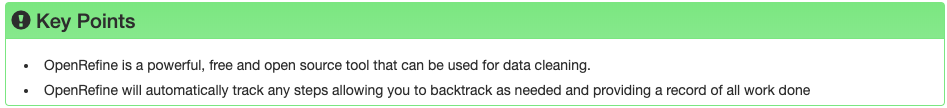
\includegraphics[width=\textwidth]{Images/OpenRefine_1.png} \\
Working With OpenRefine \\
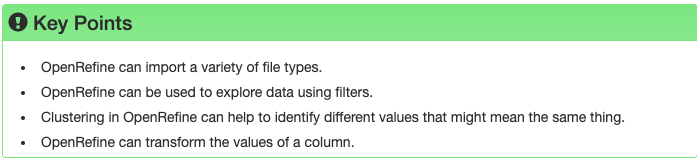
\includegraphics[width=\textwidth]{Images/OpenRefine_2.png}
Filtering and Sorting with OpenRefine \\
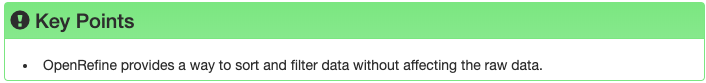
\includegraphics[width=\textwidth]{Images/OpenRefine_3.png}

\subsection{Final Thoughts}
\textbf{3:55PM} OpenRefine seems like a very useful tool with an array of feature to assist with large data sets. I enjoyed the exercises, however I found them very repetitive. This would be due to the fact I edited each column separately in the transforming data section - which I realised afterwards that you could repeat the command through the history button. That would have saved a lot of time. Next time I will make sure I read the question and solution properly before progressing with commands. \\
\textbf{4:27PM} Completed filtering and sorting in OpenRefine with few errors. I think the final errors may have been due to an internet connection - however I thought OpenRefine didn't need wifi? So maybe that isn't the case. I also was not able to find village 49 in the column so I am unsure what happened there. These exercises were predomoinately straight forward and useful in learning how to navigate, sort and utilise OpenRefine. I would like to be able to redo the final exercises with an unfrozen OpenRefine.

\section{22/09/2019}
\subsection{Thoughts/Intentions}
\textbf{12:24PM} Continue with Data Carpentry OpenRefine: Examining Numbers in OpenRefine \\
\textbf{12:53PM} Complete Using Scripts \\
\textbf{1:19PM} Complete Exporting and Saving Data from OpenRefine \\

\subsection{Actions}
Examining Numbers in OpenRefine
\begin{itemize}
\item Click years farm column 
\item Click edit cells 
\item Click Common transforms
\item Click to number
\item \textbf{SUCCESS} years farm value change from left-justified to right-justified and black to green colour
\item Click no members column 
\item Click edit cells 
\item Click Common transforms
\item Click to number
\item \textbf{SUCCESS} no members value change from left-justified to right-justified and black to green colour
\item Click years lived column 
\item Click edit cells 
\item Click Common transforms
\item Click to number
\item \textbf{SUCCESS} years lived value change from left-justified to right-justified and black to green colour
\item Click buildings in compound column 
\item Click edit cells 
\item Click Common transforms
\item Click to number
\item \textbf{SUCCESS} buildings in compound value change from left-justified to right-justified and black to green colour
\item Click village column 
\item Click edit cells 
\item Click Common transforms
\item Click to number
\item \textbf{SUCCESS} and \textbf{ERROR} Column did not change to numbers however in Undo/redo tab the action displayed "text transform on 1 cell in column village: value.toNumber". Should be 0 as no data was transformed. 
\item Editing cell in years farm column to replace 11 with text "TEST"
\item Click pull down menu and click numeric facet
\item \textbf{SUCCESS} Numeric facet appears in left panel
\item Click x in upper left corner
\item Click on steps to undo in undo/redo column
\item \textbf{SUCCESS} Steps are undone
\end{itemize}
Using Scripts
\begin{itemize}
\item Click Extract 
\item Select ALL
\item Open TextEdit
\item Copy code from operation history
\item Paste into TextEdit
\item Select format in TextEdit
\item Select Make plain text
\item Select save the file as .txt file
\item \textbf{SUCCESS} File saved as plain text file with code 
\item Create new project with messy data set
\item Named "Script Test"
\item Click undo/redo tab 
\item Click Apply
\item Paste contents of txt file 
\item Click perform operations
\item \textbf{SUCCESS} Messy data set is now the same as clean data set
\end{itemize}
Exporting and Saving Data from OpenRefine
\begin{itemize}
\item Click export button in top right
\item Select export project
\item Select download 'local'
\item \textbf{SUCCESS} local tar.gz file downloaded
\item Double clip tar zip and open
\item \textbf{SUCCESS} All components of file included i.e. history, change, data text
\item Import project in home screen
\item \textbf{SUCCESS} Imported downloaded tar zip
\item Click export
\item Click tab-separated values
\item \textbf{SUCCESS} File exported to default download directory 
\end{itemize}


\subsection{Key Points}
Examining Numbers in OpenRefine \\
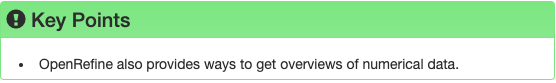
\includegraphics[width=\textwidth]{Images/OpenRefine_4.png} \\
Using Scripts \\
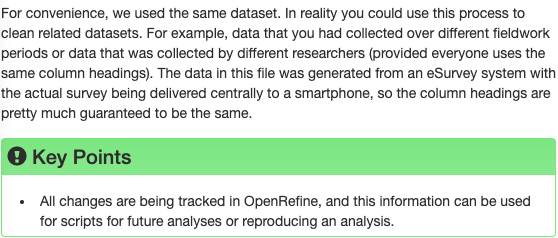
\includegraphics[width=\textwidth]{Images/OpenRefine_5.png} \\
Exporting and Saving Data From OpenRefine \\
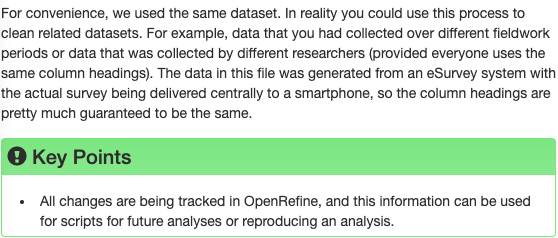
\includegraphics[width=\textwidth]{Images/OpenRefine_6.png}

\subsection{Final Thoughts}
\textbf{1:30PM} These lessons were enjoyable and straight forward. I found the using script activity extremely useful. This effectively demonstrated what we have been learning and how computational thinking can exceedingly improve time-management. 

\clearpage 

\section{03/10/2019}
\subsection{POC Tests: Upload Workflow}
I've redesigned and broken down some of the user stories in my project management system to cater for smaller and more manageable tests. I've also realised that DEVONthink 3 is a closed source and i have limited time to work with it + prompts for payment, therefore I am putting that in my backlog and working with Tropy. See figure 3 below.
\subsection{Thoughts/Intentions}
\textbf{11AM:}  Uploading photos from my iPhone onto my laptop using an iPhone USB cable and document the process.
\\
\textbf{11:30AM} After attempting and reading that photos can not be uploaded directly to Tropy, I will upload photos onto Mac photo application and move photos into Tropy
\\
\begin{figure}[H]
    \centering
    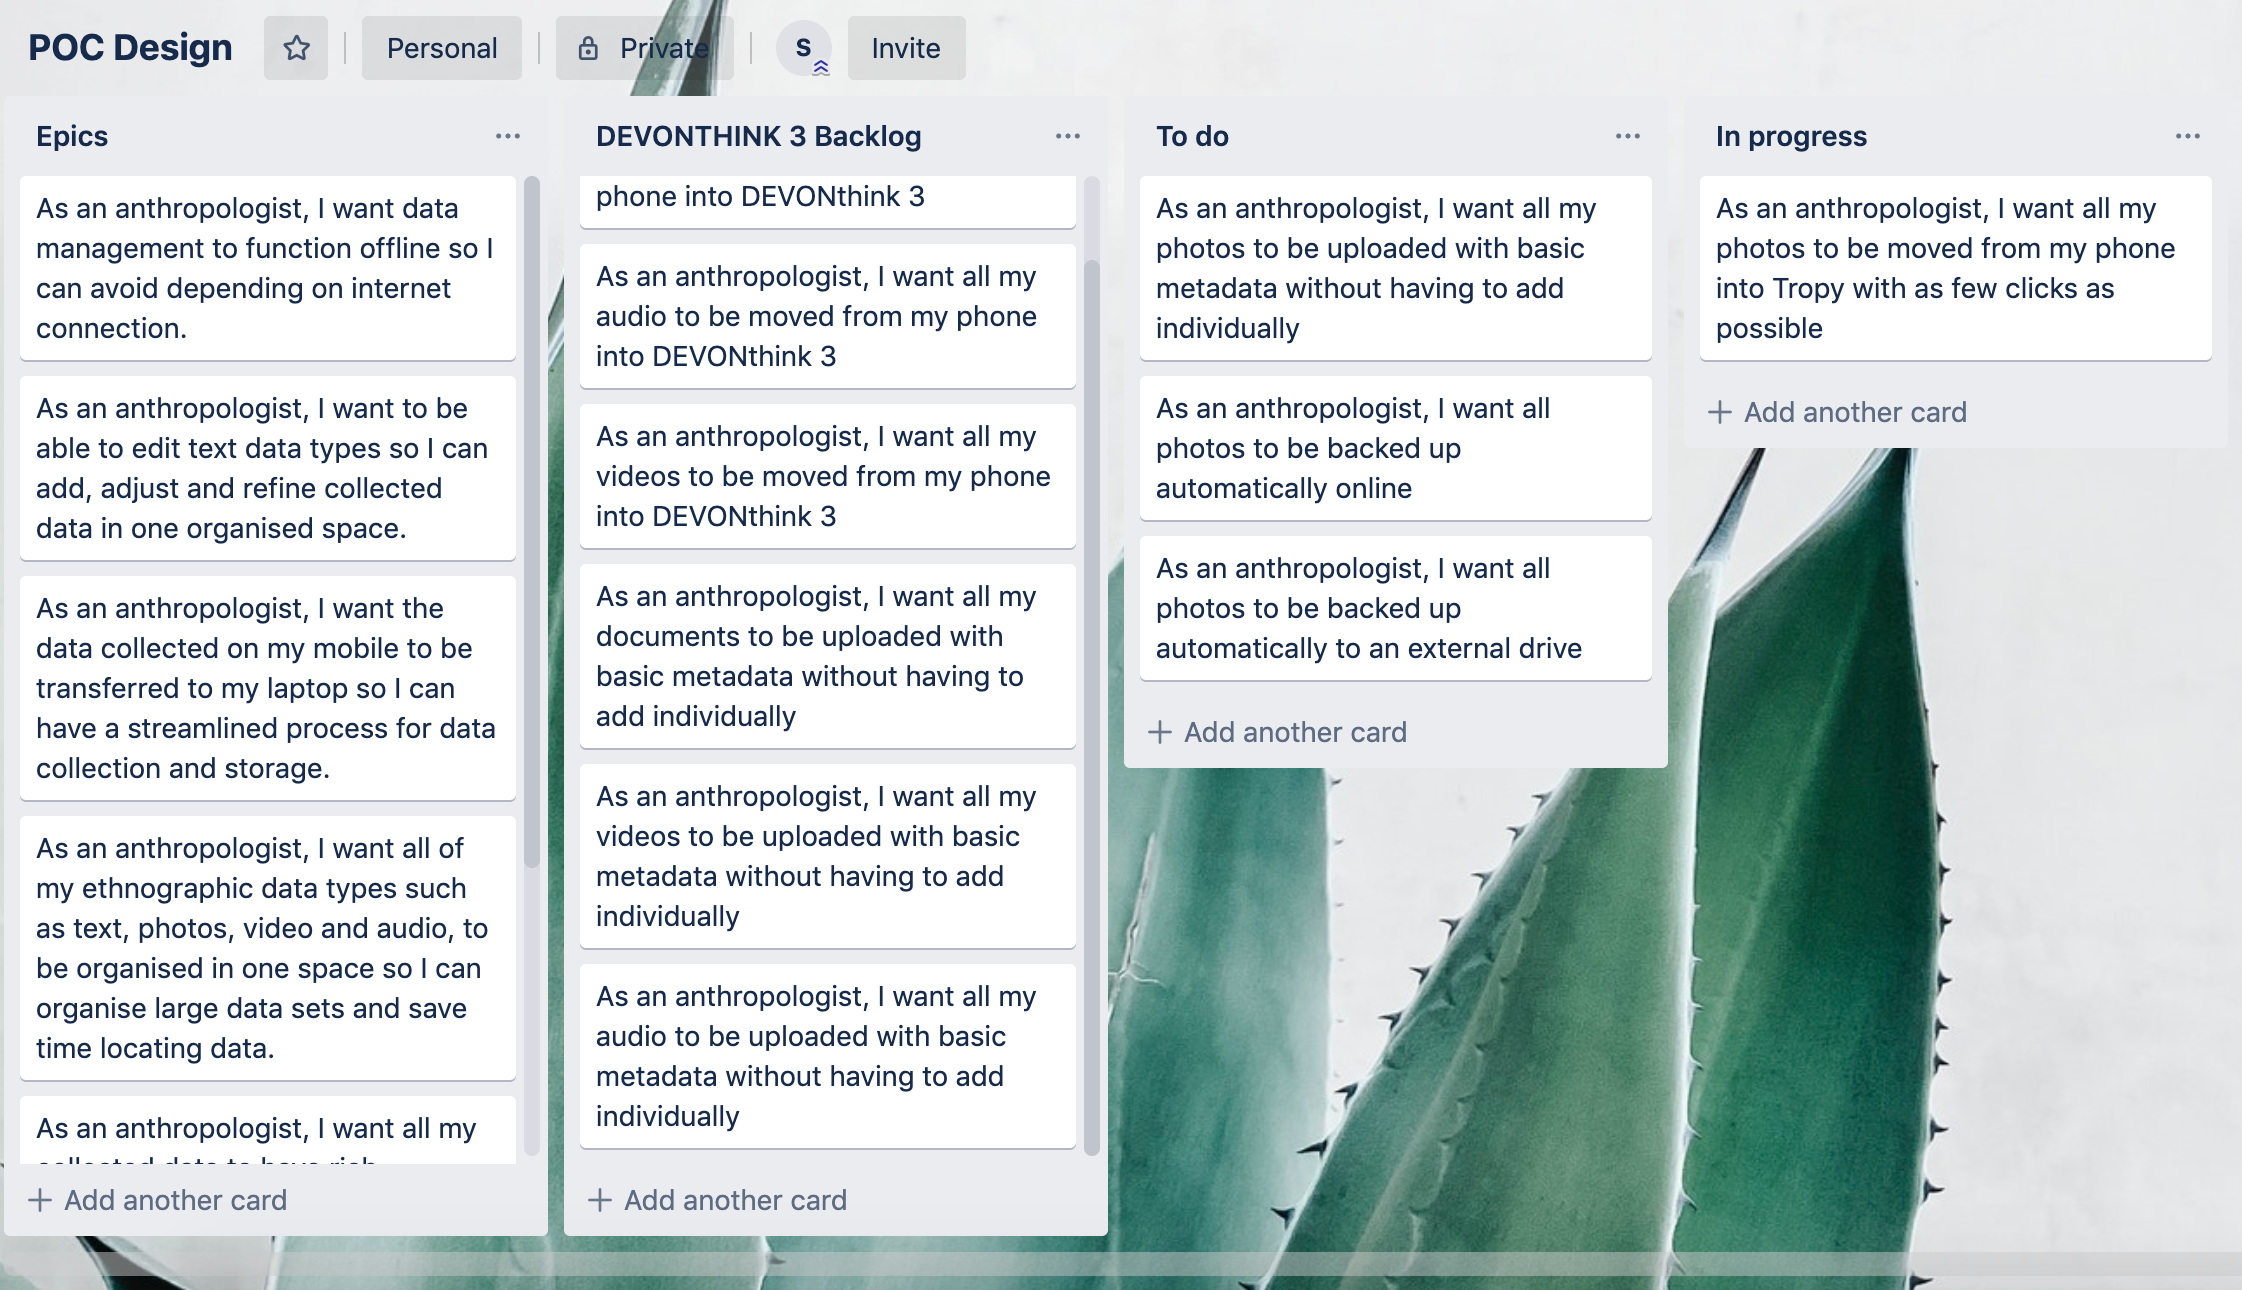
\includegraphics[width=\textwidth]{Images/Trello1.png}
    \caption{Project Management Report}
    \label{fig:my_label}
\end{figure}

\subsection{Actions}
Connecting Phone
\begin{itemize}
\item Plug iPhone into laptop using USB cord
\item iTunes pop up "Do you want to allow this computer to access information on "Sophie"
\item Click continue
\item iTunes pop up "to allow access please respond on iPhone"
\item Pop up on iPhone "Trust this Computer? Your settings and data will be accessible from this computer when connected wirelessly of using a cable"
\item Click "Trust"
\item Iphone pop up "Enter device password to trust this computer"
\item Entered password
\item iTunes pop up "a new iPhone software version (13.1.2) is available for the iPhone "Sophie". Would you . like to download it an update you iPhone now?
\item Click download and update
\item iTunes pop up "There are purchased items on the iPhone "Sophie" that have not been transferred... you should transfer these items to your iTunes library before continuing"
\item Click cancel
\item Click finder to open
\item Click applications to open
\item Double Click Tropy to open
\item Click file on Tropy
\item Click import photos on Tropy
\item \textbf{ERROR} No option to import directly from phone into Tropy
\end{itemize}
Process from Mac Photos App to Tropy
\begin{itemize}
\item Double click Photos application on mac
\item Click "Open photos for this device" next to Sophie Iphone
\item Click "Import all new items" 
\item 823 items importing into Photos application
\item \textbf{SUCCESS} Photos have been imported into Photos application on Mac
\item Click "Photos" in library section of application
\item Click "Moments"
\item Drag todays photo into Tropy
\item \textbf{ERROR} Photo does not drag from Mac application into Tropy
\item Drag photo onto desktop
\item Drag photo into Tropy
\item \textbf{SUCCESS} Photo is now in POC demonstration project in Tropy (previously created for elaboration)
\end{itemize}

\subsection{Final Thoughts}
\textbf{11:54AM} The process of uploading photos from iPhone to Mac and then into Tropy took a lot more steps that I thought it would. I now have to wrap my head around how I can make this an easier process. I think I will try using Mac Automator next to get this process moving quickly - however I have never used it before so I am unsure what the outcome will be or if I am jumping ahead. However I think I have achieved some of my acceptance criteria because using the USB cord allows a lot of data to be moved at once and works offline so that is good. 

\section{03/10/19}
\subsection{POC Tests: Upload Workflow}
I want to attempt using Mac Automator after hearing about its ability to streamline repetitive tasks and create workflows. This program could be really useful as it is free, works offline and is already available on my laptop.
\subsection{Thoughts/Intentions}
\textbf{5:13PM} Exploring Mac Automator. Not expecting I will be able to configure anything but would like to get familiar with the program. \\
\textbf{5:36PM} Found record workflow option, so I'm going to upload photos, drag them into a desktop folder named "sort photos", and then drag them into Tropy. I won't be able to type each step so will record outcome. \\
\textbf{5:59PM} Recording workflow. This time I will replicate the test run from beginning with plugging in phone, having new photos to import, and making sure everything is closed so the test can restart. See Figure 5: Attempt 2: Displays Error pop up.

\subsection{Actions}
\begin{itemize}
\item Double click Automator
\item Pop up appears "Choose a type for your document - workflow, application, quick action, print plugin, folder action, calendar alarm, image capture plugin or dictation command"
\item Figure I should google how to use Mac Automator before selecting
\item Going to select workflow to begin
\item Selecting record workflow 
\item After recording workflow select Run
\item \textbf{ERROR} "Watch Me Do Failed - 1 error The action "Watch Me Do" encountered an error: The operation couldn't be completed. See Figure 4: Attempt 1. 
\end{itemize}

\begin{figure}[H]
    \centering
    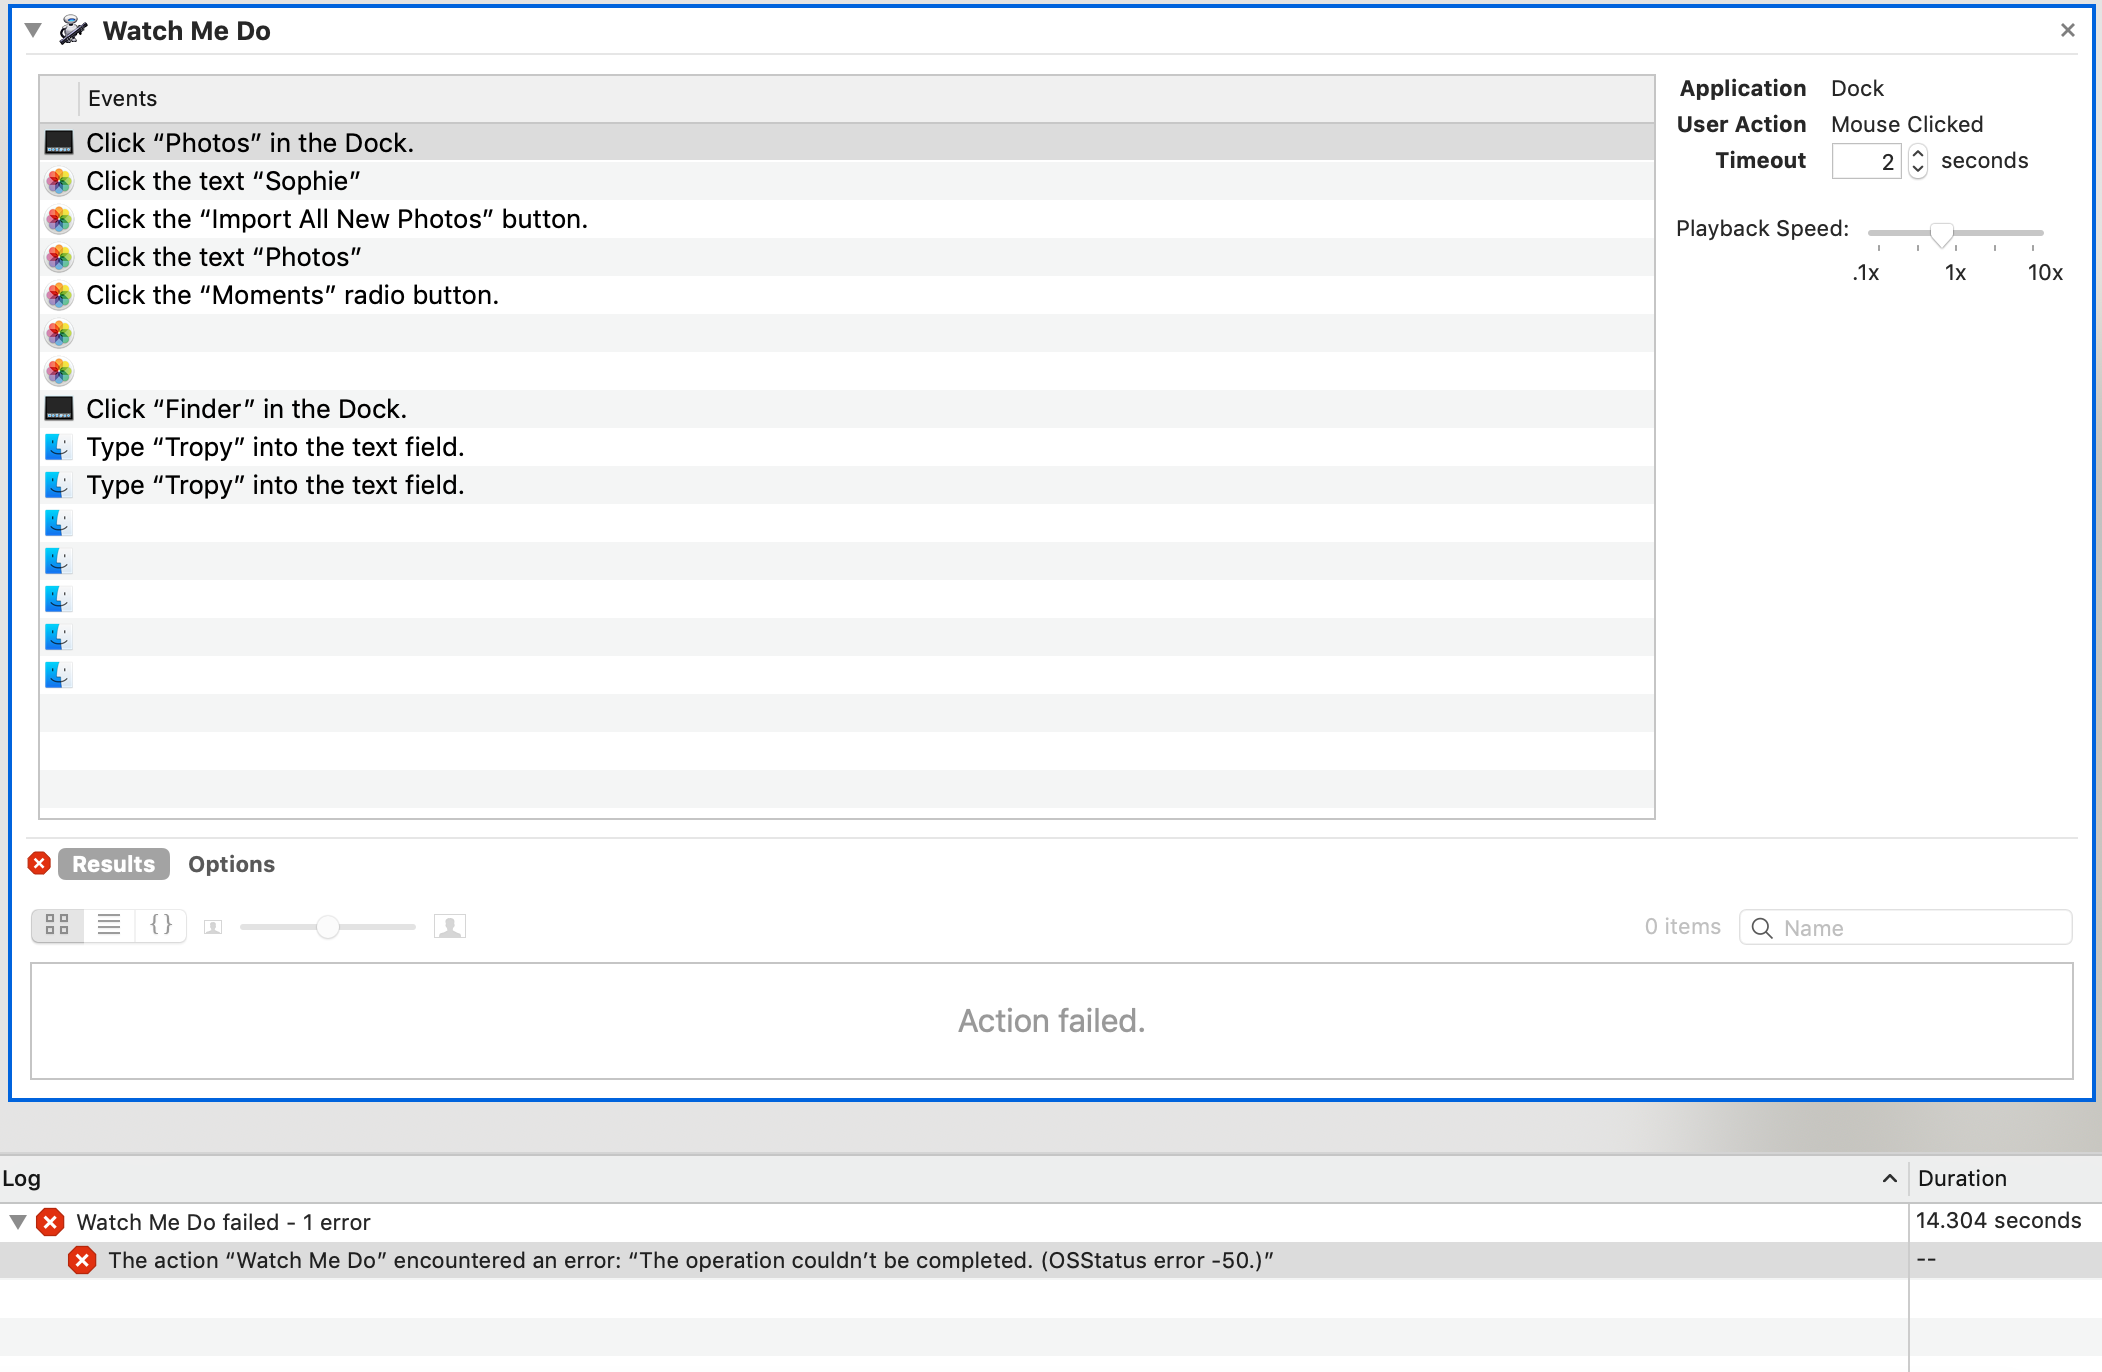
\includegraphics[width=\textwidth]{Images/Automator_1.png}
    \caption{Attempt 1}
    \label{fig:my_label}
\end{figure}

\begin{figure}[H]
    \centering
    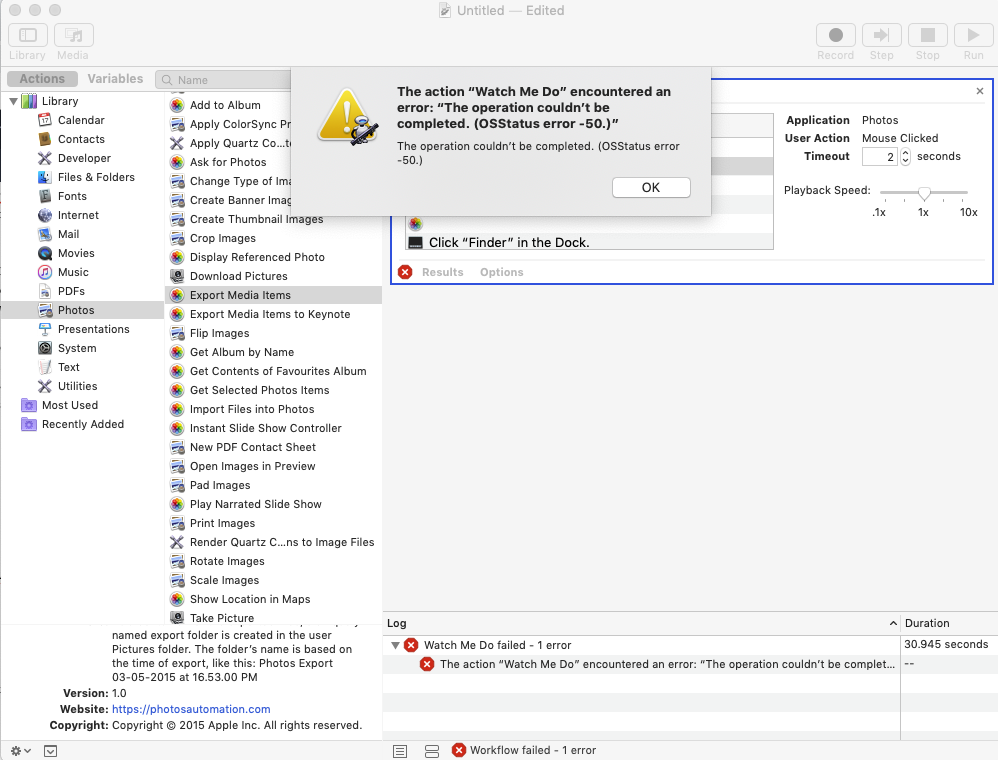
\includegraphics[width=\textwidth]{Images/Automator_2.png}
    \caption{Attempt 2 Displays Error Pop-up}
    \label{fig:my_label}
\end{figure}

\subsection{Final Thoughts}
\textbf{5:49PM} I think I know why this error occurred. I clicked import All New Photos button during my recording, then when I went to run the test there were no photos available to import. Will try test again with photos available. \\
\textbf{6:30PM} I still had trouble trying to use the Automator despite having photos available for importing. I think it could be my dragging motion that selects images is unclear, however I am unsure. I will need to look further into using Automator before I run another test. An external error that was frustrating is my mac Photos application kept freezing and I had to force quit the application, so that could have contributed to the Automator not working. I definitely think this program will be efficient once I work out how to use it properly, I will just need to run more tests after doing some research.

\section{04/10/19}
\subsection{POC Tests: Upload Workflow}
After briefly looking at some Automator tutorials I want to try create a basic Automator service to move files. In the tutorial this was called "services" however in my mac Automator it is called a "quick action". 
\subsection{Thoughts/Intentions}
\textbf{12:07PM} Create basic Automator quick action.
\textbf{12:15PM} Attempt to move photos from inside mac Photo application using quick action.

\subsection{Actions}
Basic Move File
\begin{itemize}
\item Open Automator
\item Click create new document
\item Select Quick Action
\item Select files and folders in left panel
\item Select Move Finder items
\item Select destination to folder Sort photos
\item Save quick action under title "Move to sort photos"
\item Left click on desktop image
\item \textbf{SUCCESS} Move to sort photos quick action is available and does required action. See Figure 6 below.
\end{itemize}
Move file directly from inside Photo App
\begin{itemize}
\item Open Photos
\item Left click on photo
\item \textbf{ERROR} No quick action available
\end{itemize}

\begin{figure}[H]
    \centering
    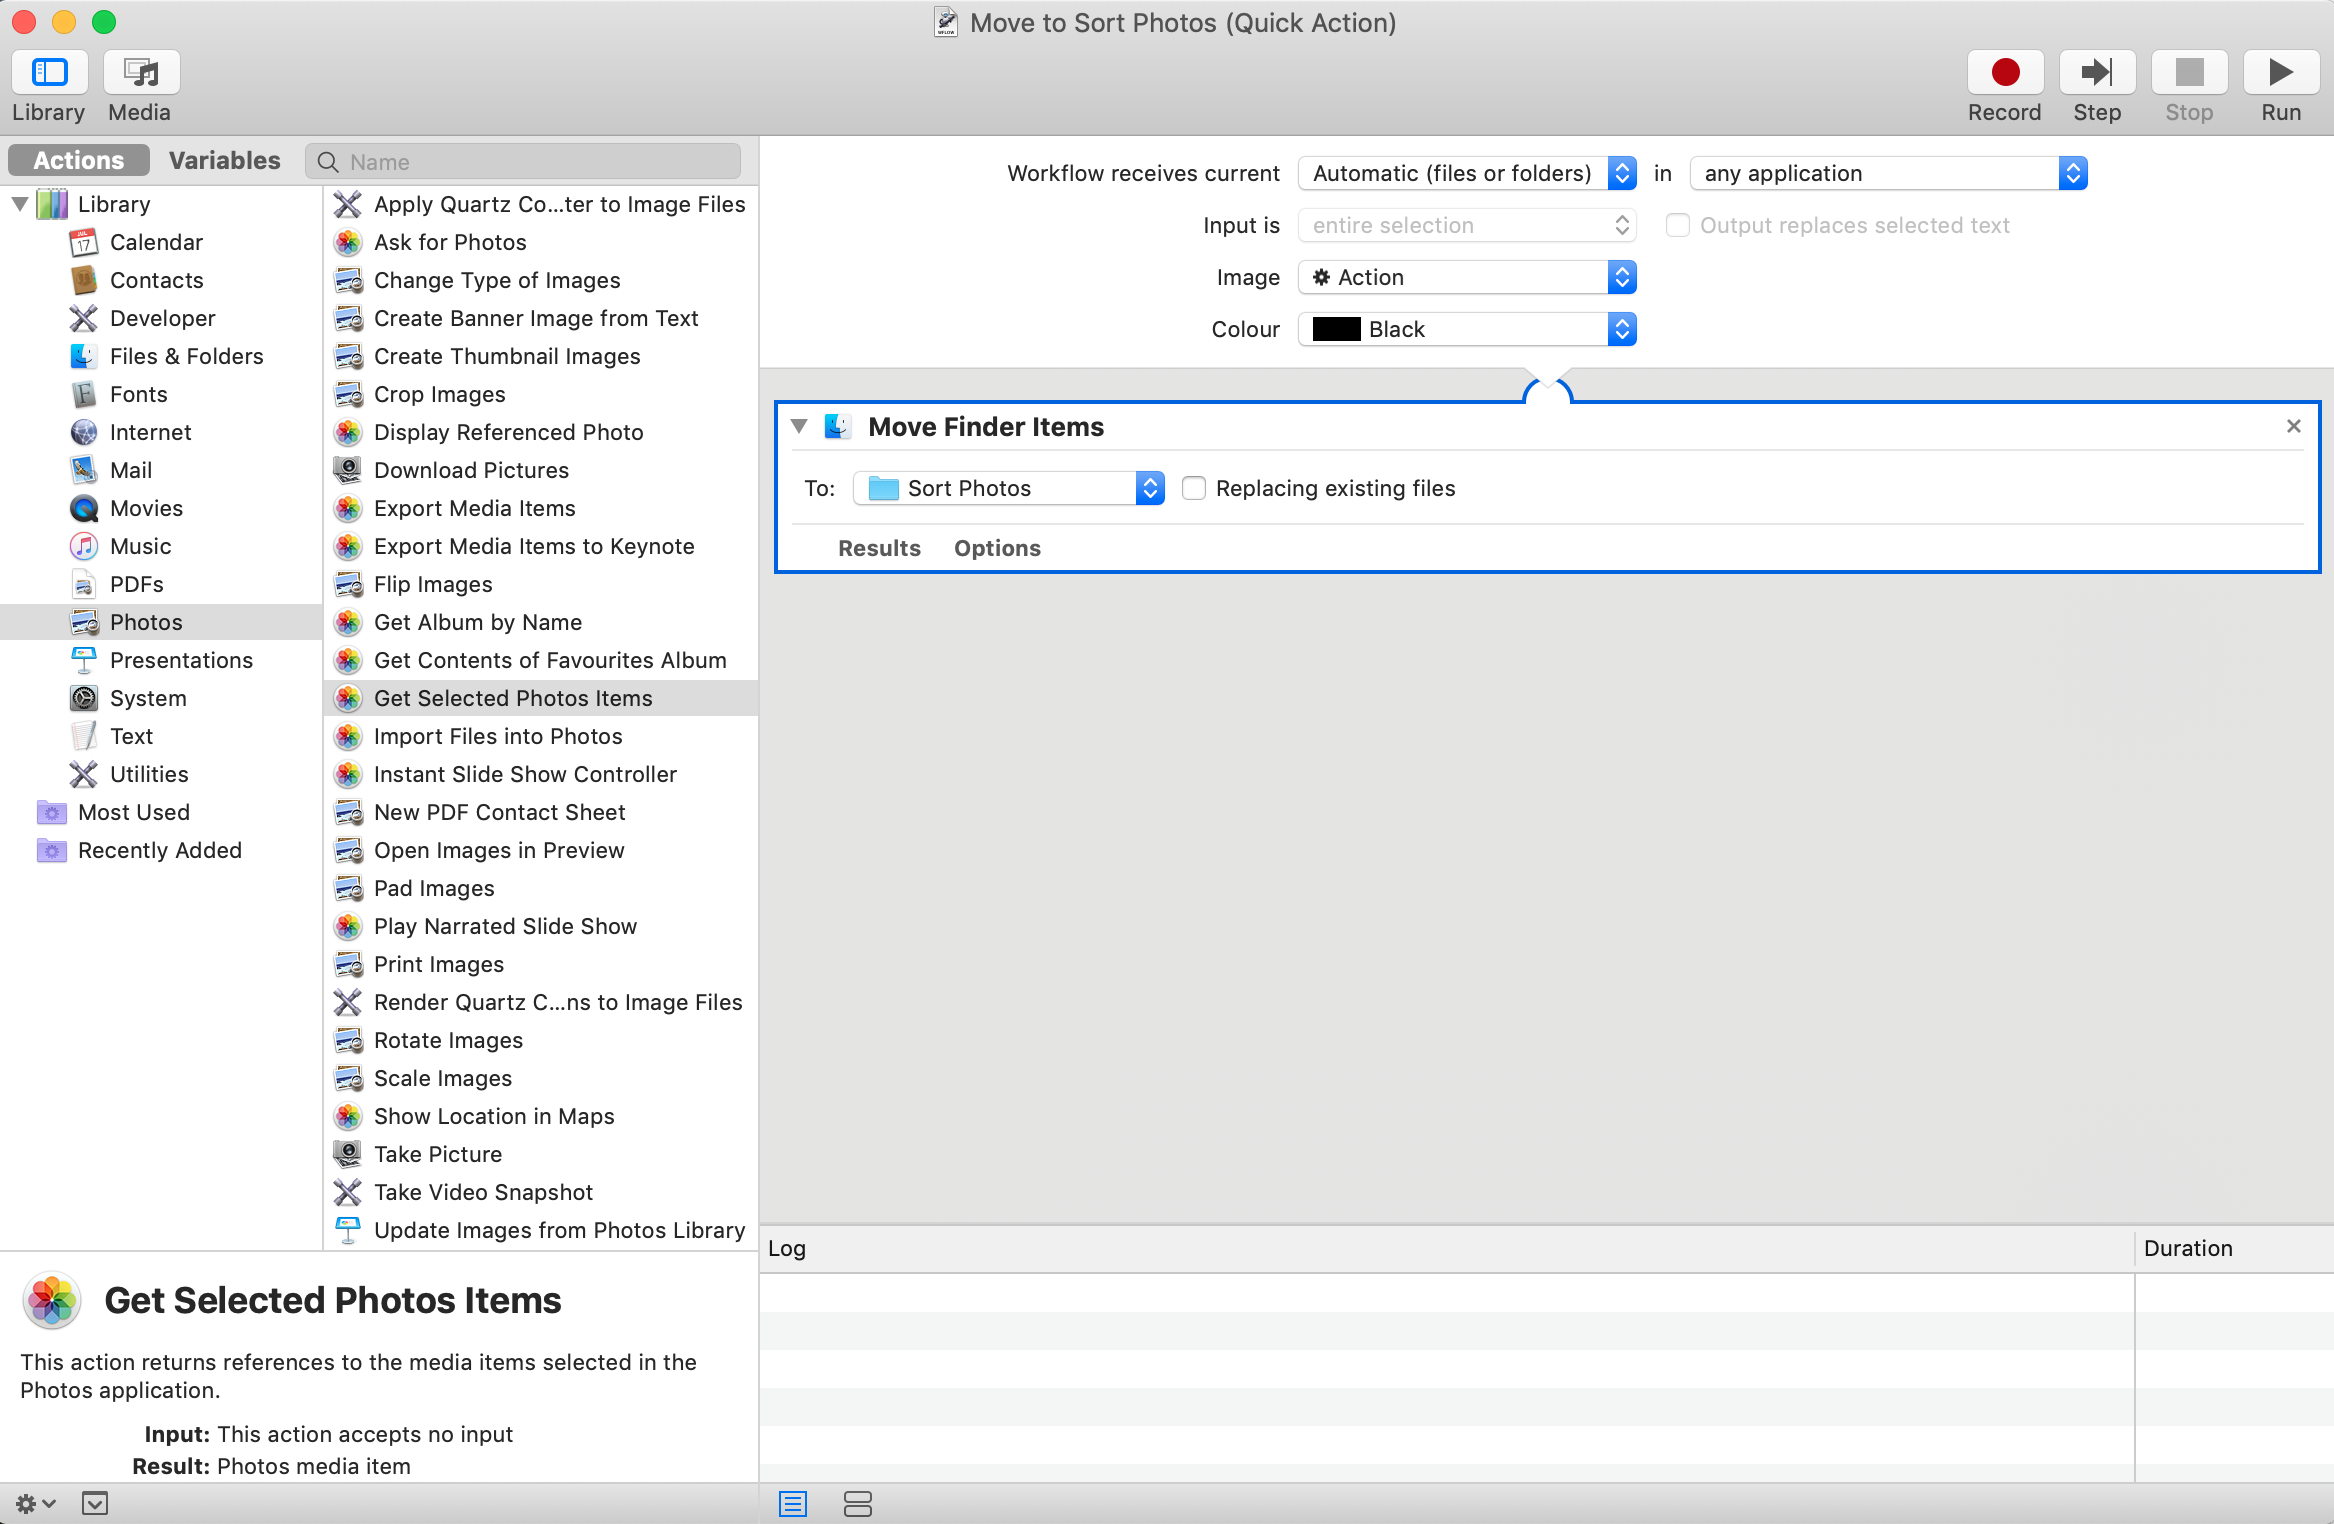
\includegraphics[width=\textwidth]{Images/Automator_3.png}
    \caption{Successful Quick Action}
    \label{fig:my_label}
\end{figure}

\subsection{Final Thoughts}
\textbf{12:23PM} I still feel out of my depth and need to read more about mac automator. I can create a very simple quick action that moves photos outisde of an application. A lot of the actions look like they would be helpful, I just have to play around a lot more - it is hard to play around freely and document at the same time because I feel like I double think each step due to having to write it down. I think if I could just mess  around with  documentation this process may be a lot quicker. Actions I want to explore are:
\begin{itemize}
\item Running Automator in application
\item Running action "Get selected photo items"
\end{itemize}

\section{08/10/201}
\subsection{POC Tests: Upload Workflow}
The last session was a struggle so i've looked up some more youtube tutorials for mac automator and found some more guidance. 
\subsection{Thoughts/Intentions}
\textbf{12:12pm} Attempt to create basic automator workflow to export uploaded photos into external album

\subsection{Actions}
\begin{itemize}
\item Open Photos
\item Create album in photos as "Export"
\item Open automator
\item Select workflow option
\item Add "Get Album by Name" action
\item Add "Export" into album select
\item Add action "Export Media Items"
\item Change Naming method: name in numeric sequence"
\item Write Base name as: fieldwork
\item Plug in iphone
\item Select upload new photos into Export album
\item Run workflow 
\item \textbf{SUCCESS} Export album was moved into pictures folder under the name "Photos Export 2019-10-10 12.15.46 pm"
\end{itemize}

\begin{figure}[H]
    \centering
    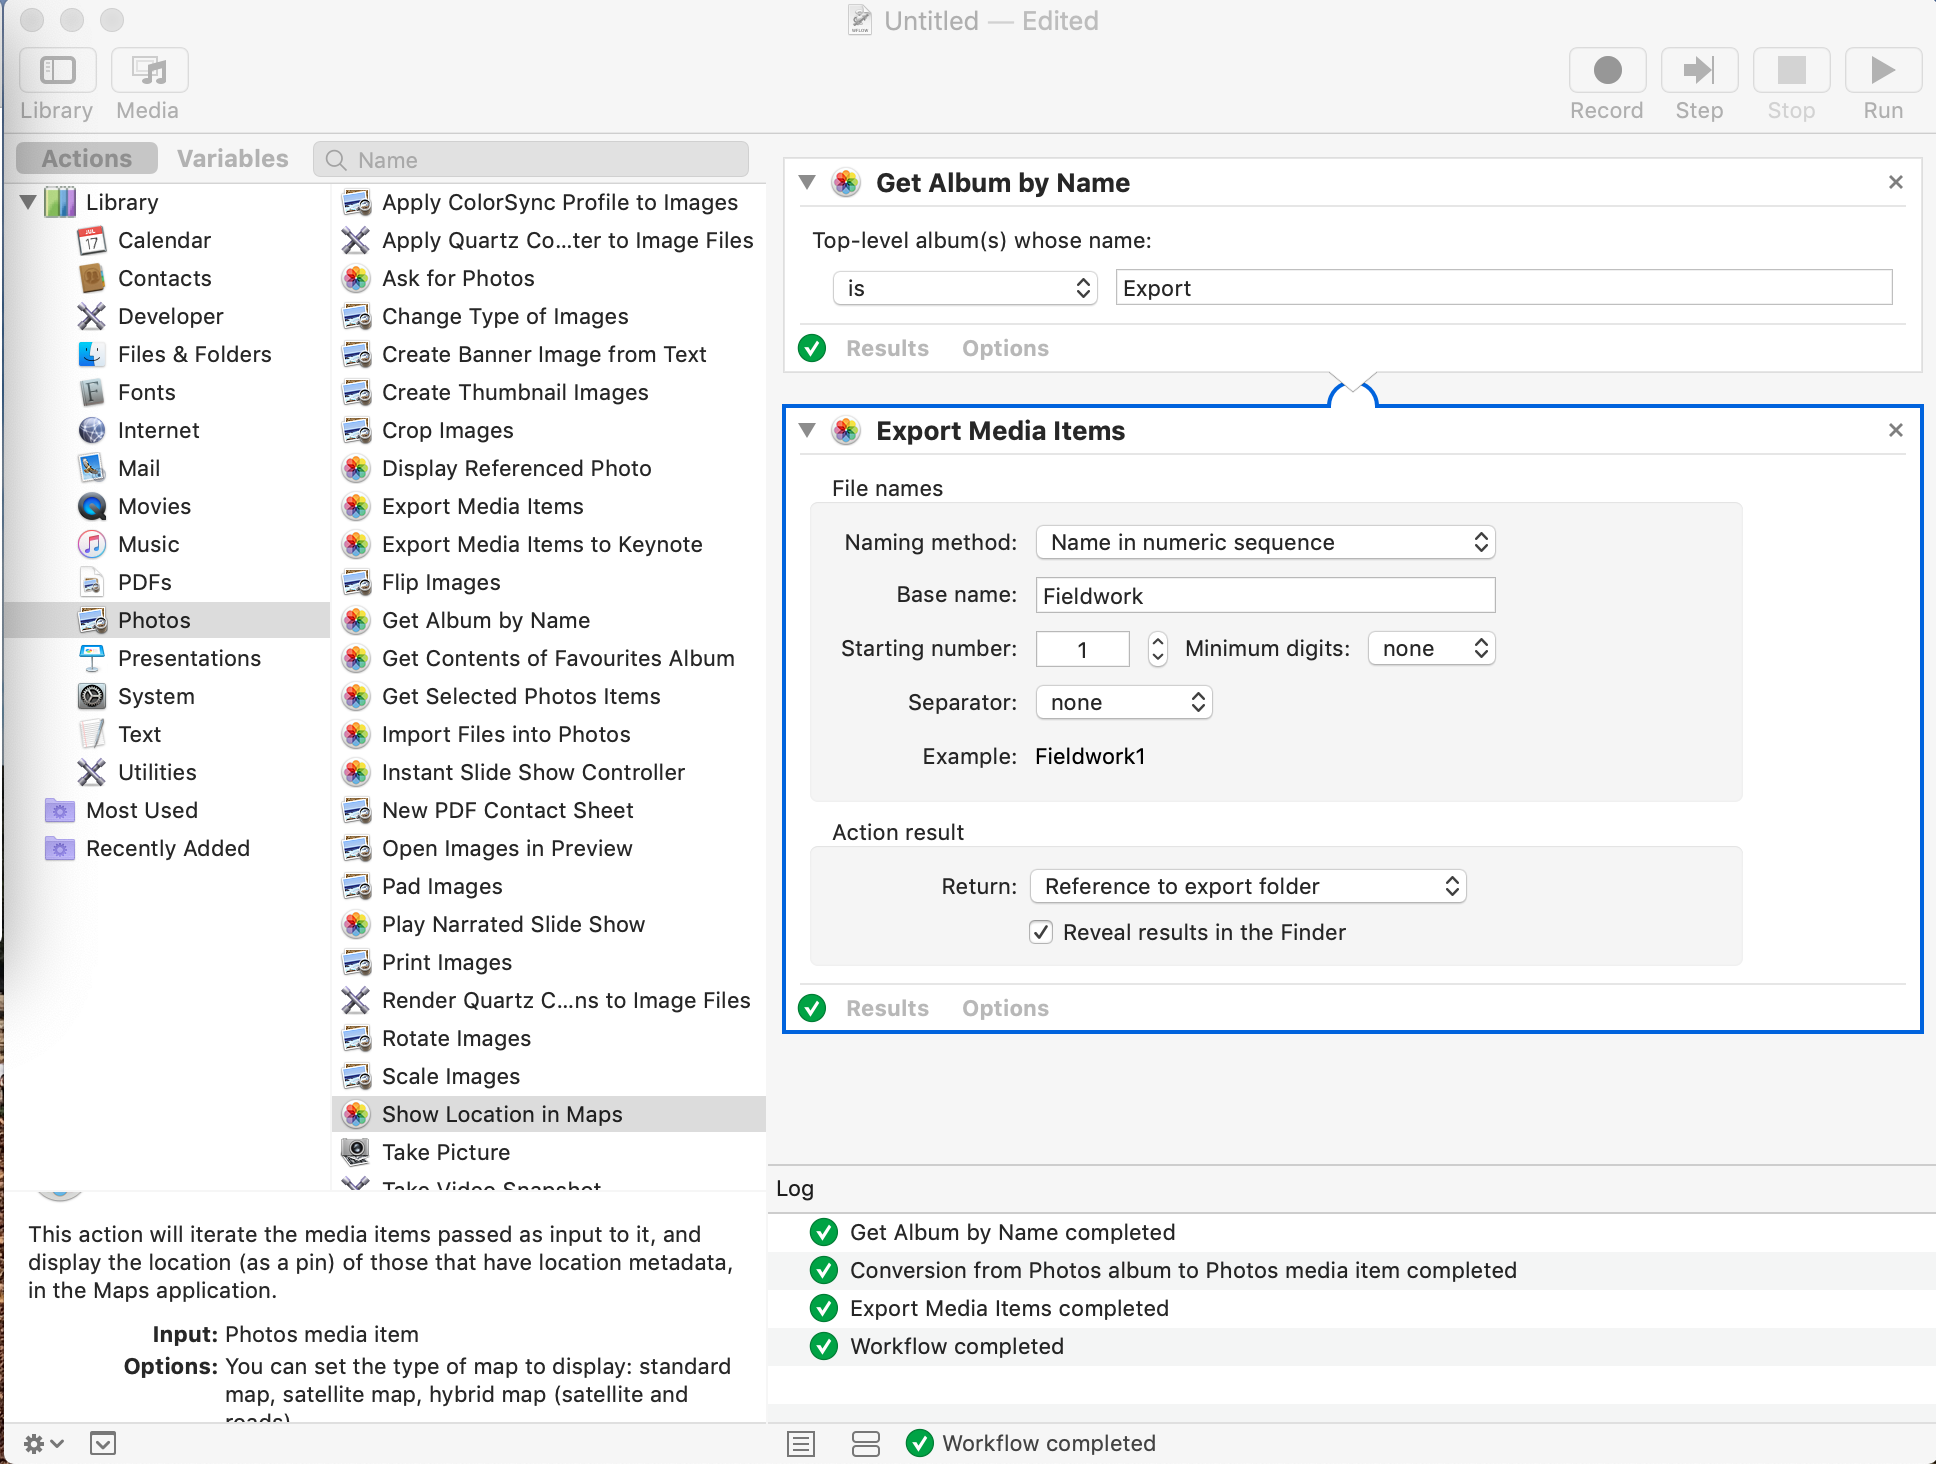
\includegraphics[width=\textwidth]{Images/Workflow_Success1.png}
    \caption{Successful Workflow}
    \label{fig:my_label}
\end{figure}

\begin{figure}[H]
    \centering
    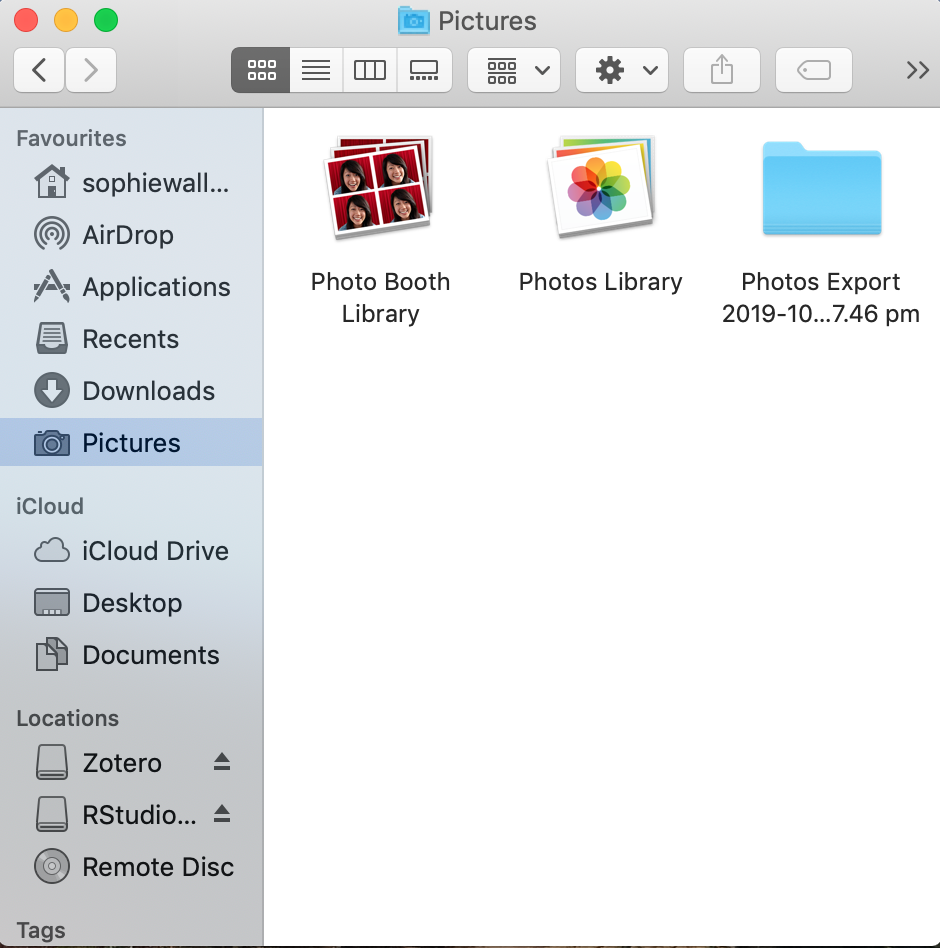
\includegraphics[width=\textwidth]{Images/PhotoExport_1.png}
    \caption{Result from Workflow}
    \label{fig:my_label}
\end{figure}
\subsection{Final Thoughts}
\textbf{12:18PM} Now that there is an exported folder in my pictures album, I have to figure out how I can move that album into Tropy and prompt with metadata, which will take more research and trial and error.

\section{11/10/2019}
\subsection{POC Tests: Upload Workflow }
I've found another action in mac automator called Download pictures. This may present a more streamlined approach to uploading photos from my iPhone directly to a folder in my desktop and by-passing the mac Photos application.

\subsection{Thoughts/Intentions}
\textbf{10:30AM} Attempt to run download pictures action in automator
\textbf{10:50AM} Now that I at least know there is a way to automate photos from my iPhone to a desktop folder (using either the previous test or attempting this one again) I really want to know how I can move photos from inside the folder into Tropy. I feel like it will be more straight forward to write a script than use automator for this however I'm overwhelmed by the commands and process.

\subsection{Action}
\begin{itemize}
\item Start new workflow document in automator
\item Select photos section in library
\item Drag "download pictures action into workflow panel
\item Plug iphone in 
\item \textbf{SUCCESS} Iphone appears in Camera Name and displays how many items are to be downloaded
\item Select download location to sort-photos folder on desktop
\item Run test
\item \textbf{ERROR} Test runs for 4 minutes and nothing happens
\end{itemize}



\subsection{Final Thoughts}
\textbf{10:46AM} I've replicated this test twice and waited for a response and it doesnt appear to do anything. The test says it is running, however the download time is taking a while with no indication that it is working. I will have to run again when I have more time to wait it out. \\

\textbf{11:50AM} After a lot of googling and trial and error in the terminal, I am nowhere close to figuring this out. Really do not know where to go from here. Doing this manually by just uploading photos and then dragging them into Tropy and then labelling them seems like a much more straight forward process at the moment. I feel like im only minimizing a few clicks despite the hours of work trying to figure it out.

\section{17/10/2019}
\subsection{Downloading Tools for POC}
After speaking with Brian I need to now download a few tools to assist with this POC. 
\subsection{Thoughts/Intentions}
\textbf{11:51AM} Going to download Exif for metadata management \\
\textbf{12:04PM} Testing exiftool to see if installed correctly \\
\textbf{12:09PM} Now that exiftool is downloaded I want to download Duplicati . \\ 
\textbf{12:21PM} Leaving Duplicati download for now and moving onto reading about Tropy templates. \\
\textbf{1:26PM} I've read about the Tropy templates now attempting to create a test template.

\subsection{Actions}
ExifTool Download
\begin{itemize}
\item Entering ExifTool by Phil Harvey website
\item Click download MacOS Package: ExifTool-11.71.dmg (2.8 MB)
\item \textbf{SUCCESS} package installer now opened on desktop
\item Double click installer
\item Prompt "“ExifTool-11.71.pkg” cannot be opened because it is from an unidentified developer."
\item Click OK
\item Installer opens - click continue through prompts
\item \textbf{SUCCESS} Installation was successful
\end{itemize}
ExifTool test
\begin{itemize}
\item Open terminal
\item Type exiftool
\item \textbf{SUCCESS} Tool name, synoposis, description, options and option details appear. 
\item See Figure 9: ExifTool in Terminal below.
\end{itemize}

\begin{figure}[H]
    \centering
    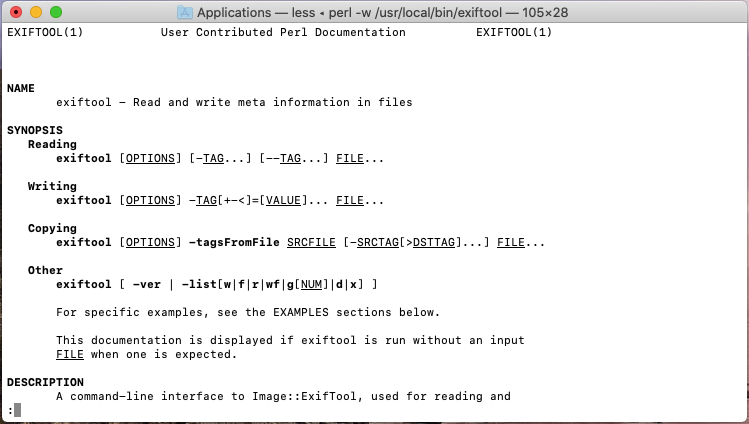
\includegraphics[width=\textwidth]{Images/ExifTool_1.png}
    \caption{ExifTool in Terminal}
    \label{fig:my_label}
\end{figure}

Duplicati Download
\begin{itemize}
\item Enter Duplicati website
\item Click download Duplicati 2.0 (beta) option
\item Click macOS / OSX 2.0.4.23 option
\item \textbf{SUCCESS} Downloaded onto desktop
\item Double click on installer
\item \textbf{ERROR} "The following disk images couldn't be opened: Image Duplicati-2.0.4.23 beta / Reason: Image not recognised.
\item Click ok
\item Right click on installer
\item Click "Open with - Disk Image Mounter (Default"
\item \textbf{ERROR} Same error message as above.
\item Open System Preferences
\item Click Security and Privacy
\item Click the lock to make changes
\item Double click Duplicati
\item \textbf{ERROR} Same error message as above.
\end{itemize}

Tropy Template
\begin{itemize}
\item Open Tropy
\item Select preferences
\item Select Template
\item Select 'locked' template with desired categories
\item Click the double page icon next to template name
\item \textbf{SUCCESS} Locked template has been duplicated and URI is different
\item Fill in Name, type, creator description.
\item Click Create
\item Option for selecting properties appears
\item Click Date
\item Label as Date
\item Default "datatype" is under name "String xsd:string" (unsure what this means)
\item See Figure 10. below for reference of filled categories and test template.
\item Click upload icon next to template
\item Save As: Tropy Template Test
\item \textbf{SUCCESS} Tropy Template test is saved on desktop
\end{itemize}

\begin{figure} [H]
    \centering
    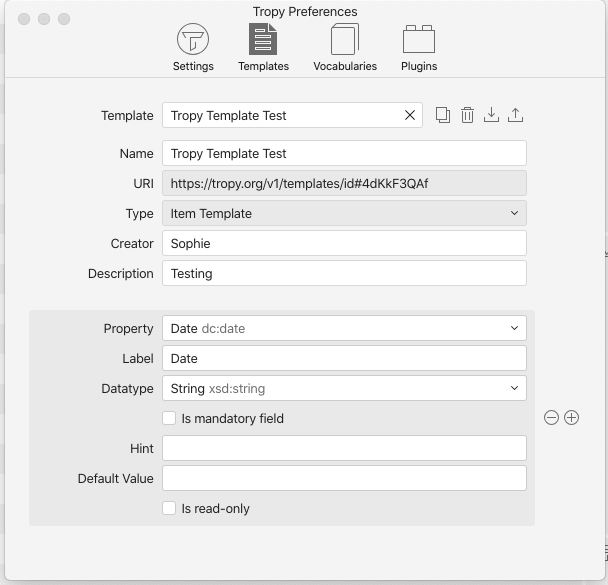
\includegraphics[width=\textwidth]{Images/TemplateTest_1.png}
    \caption{Tropy Template Test}
    \label{fig:my_label}
\end{figure}


\subsection{Final Thoughts}
\textbf{1:36PM} I'm glad that I have been able to download ExifTool and begin playing around with Tropy Templates, however I'm not sure what happened with Duplicati or what the next step is with the tropy template - or how that will work. I will continue on this later after returning to some major essays that are due soon.

\section{18/10/2019}
\subsection{POC test: Upload Workflow}
After messing around with Automator I have found how to export from photos into a desktop folder and have them renamed with the base name ChanguField (Changu being the name of the place and Field referring to fieldwork). They are ordered sequentially and also have the date added. They currently export to a folder on my desktop named Organise. 

\subsection{Thoughts/Intentions}
\textbf{7:46PM} Document automation process. See Figure 11 for brief automation.

\subsection{Actions}
\begin{itemize}
\item Enter Automator
\item Select workflow
\item Add action "get album by name" and write desired album in photos (in this case Export)
\item Add action Export Media Items
\item Choose file name (faulty for me, I rename later)
\item Choose action result: Resturn: Reference to export folder
\item Add action Move Finder Items to desired album (i.e. Organise)
\item Add action Get Folder Contents
\item Add action Rename Finder Items: Make sequential
\item Select option new name and write desired name (i.e. ChanguField)
\item Select separated by underscore
\item Add action Rename Finder Items: Add Date or Time
\item Select separated by underscore
\end{itemize}

\begin{figure}[H]
    \centering
    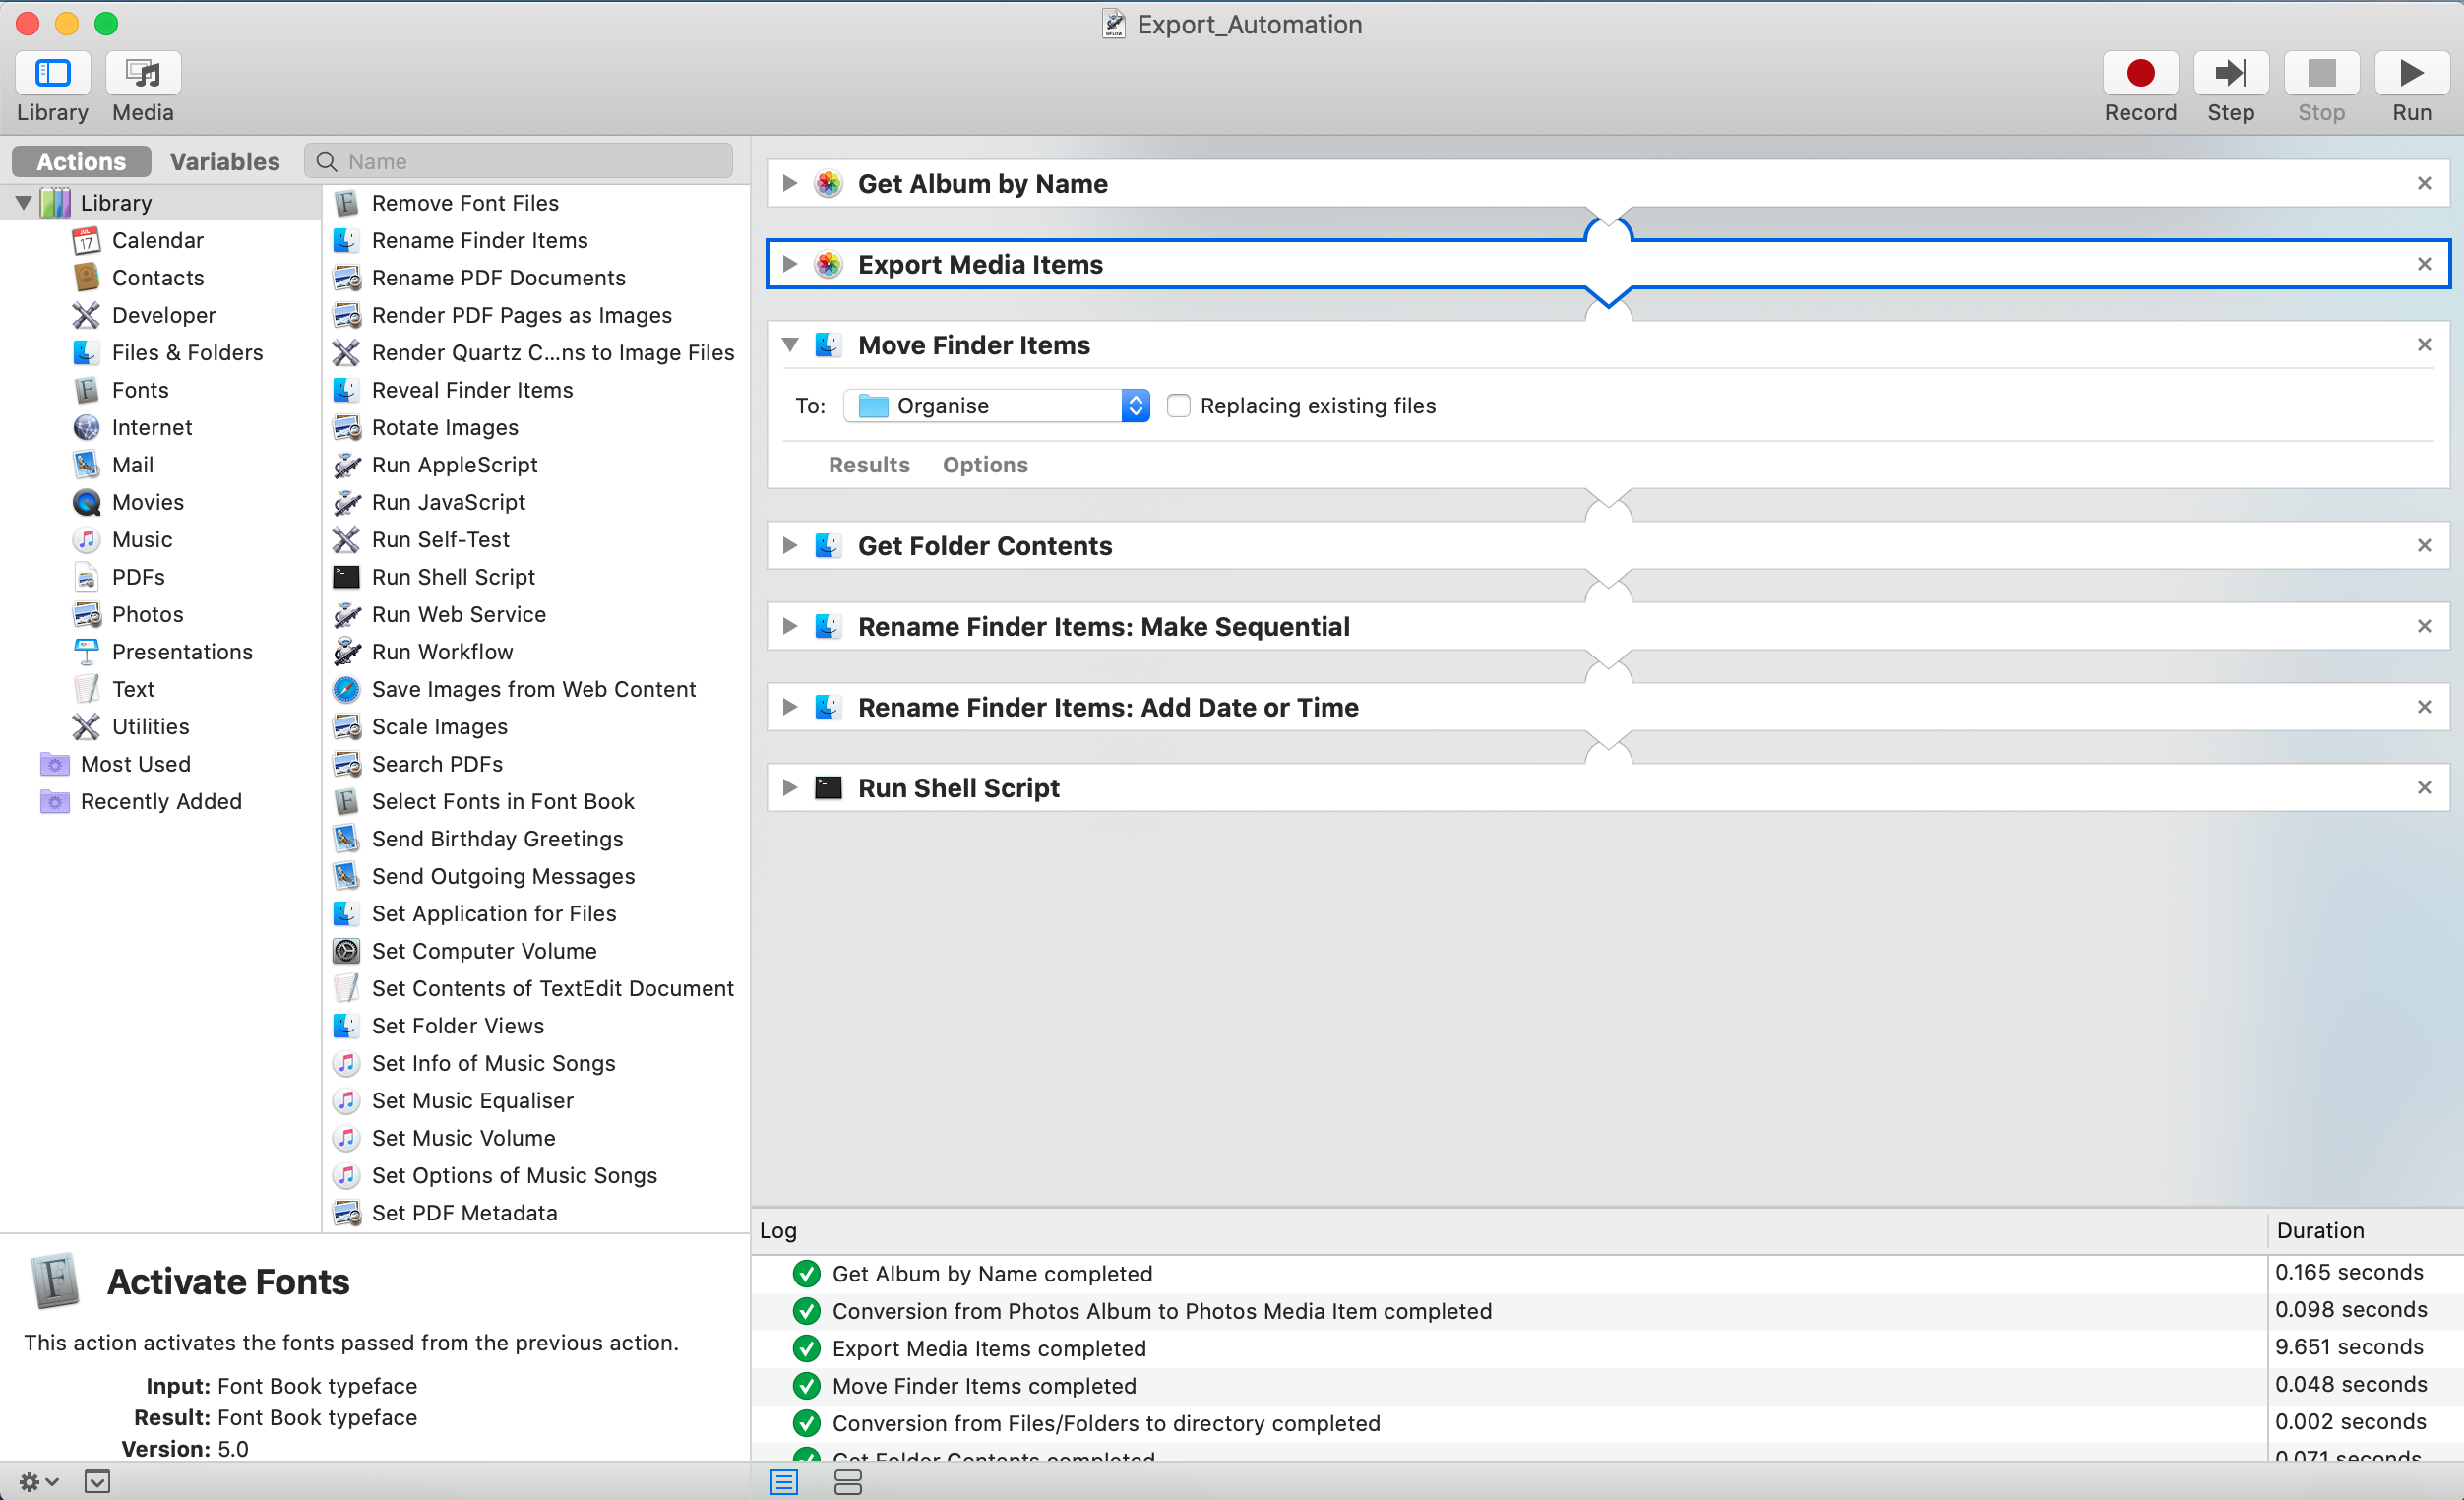
\includegraphics[width=\textwidth]{Images/Automator_4.png}
    \caption{Successful Workflow}
    \label{fig:my_label}
\end{figure}

\subsection{Final Thoughts}
\textbf{8:02PM} At least one of my functions are complete, however I still have a long way to go with exif, tropy template and shell script. As you can see above in figure 11, automator uses shell script so I might have to run some shell script in there to get the photos into Tropy. I am most nervous about the shell script as that seems like the most difficult section that I am the most incapable of. Same with exif, however we shall see.

\section{18/10/2019}
\subsection{POC test: Working With ExifTool}
I have this tool for metadata that I need to learn how to use. I'm currently attempting to work with exiftool in shell to extract metadata from the images I will use for this POC.

\subsection{Thoughts/Intentions}
\textbf{8:48PM} Document actions in ExifTool \\
\textbf{9:03PM} After many errors I found the solution, documenting action. \\
\textbf{9:33PM} Testing different commands found online for ExifTool

\subsection{Action}
\begin{itemize}
\item Enter shell terminal
\item type exiftool
\item \textbf{SUCCESS} exiftool program is displayed in shell
\item drag photo into exiftool
\item \textbf{ERROR} Pattern not found (press return)
\item Type E for examine
\item Drag photo in
\item \textbf{SUCCESS} or \textbf{ERROR}? Unsure, copious amounts of blacked out code
\item Press esc, command l and other commands to exit 
\item \textbf{ERROR} The default error noise is made, unsure how to continute
\item Click exit in top left corner
\item Prompt do you want to terminate this session? Select yes
\item \textbf{SUCCESS} and \textbf{ERROR}, exited session however not accurately.
\end{itemize}
Successful Attempt
\begin{itemize}
\item Open shell terminal
\item type exiftool
\item add space next to exiftool
\item drag photo into shell
\item press enter
\item \textbf{SUCCESS} Photo metadata is displayed in shell
\item command K to refresh terminal
\item type exiftool
\item add space
\item drag six images in at once
\item \textbf{SUCCESS} Metadata for all six images are displayed
\end{itemize}
ExifTool Commands
\begin{verbatim}
   type exiftool -d "%r %a, %B %e, %Y" -DateTimeOriginal -S -s *.jpg 
\end{verbatim}
\begin{itemize}
\item drag image next to code
\item press enter
\item \textbf{ERROR} no matches found: *.jpg
\item type "" without .jpg  
\item drag image next to code
\item press enter
\item \textbf{SUCCESS} original date and time displayed
\end{itemize}

\subsection{Final Thoughts}
\textbf{9:24PM} I'm really happy I figured out how to see metadata of photos in exiftool relatively quickly. I was worried it would take a lot of time like everything else, so very relieved. I like that it has the original time and date in the photo, however I am unable to see location so I'm unsure what to do there. \\
\textbf{9:52PM} This command draws out original date and time, which I feel could be very useful down the track. If I had the location I would be satisfied. See Figure 11 below for neat display in shell with commands. 

\begin{figure}[H]
    \centering
    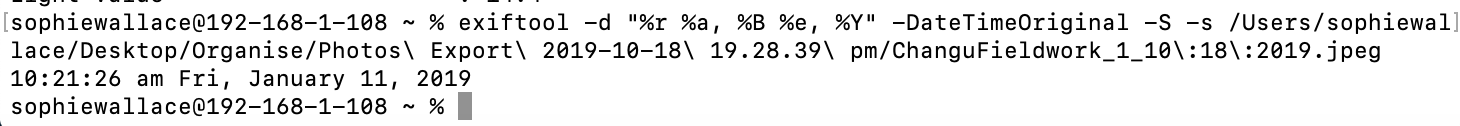
\includegraphics[width=\textwidth]{Images/ExifTool_Command.png}
    \caption{Successful Shell Commands}
    \label{fig:my_label}
\end{figure}

\section{21/10/19}
\subsection{Thoughts/Intentions}
\textbf{8:49PM} Hoping to get through some of data carpentry, I have a lot of assessments due at the moment and want this out of the way. \\
\textbf{9:14PM} Due to the lengthy nature of these tasks, I'm going to take screenshots of my work in the console and write whether they are a success or not. Working in Creating Objects in R

\subsection{Actions}
Create New Project
\begin{itemize}
\item Click new project in file menu
\item Select new directory
\item Click new project
\item Enter a name "R-Tasks"
\item Create folder names data-carpentry in home 
\item Click create project
\item \textbf{SUCCESS} new project named R-Tasks inside data-carpentry folder in home
\end{itemize}
Downloading the data and getting set up
\begin{itemize}
\item Copy and paste these commands (see below) in the R console to create folders in the working directory
\item \textbf{SUCCESS} The folders are now in the working directory
\end{itemize} 

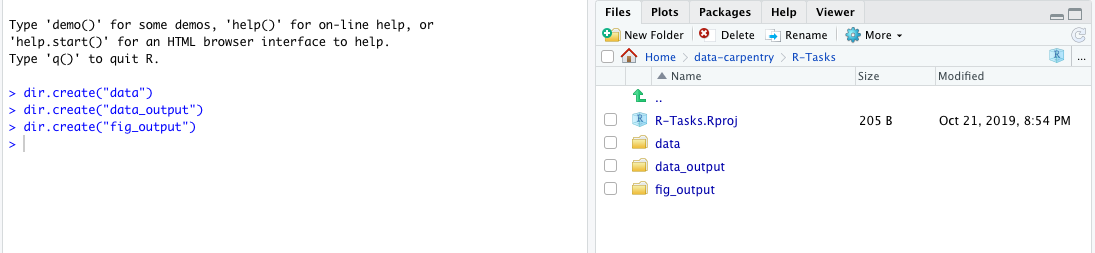
\includegraphics[width=\textwidth]{Images/RStudio_1.png} 

\begin{itemize}
\item Type in given commands for downloading safi data . set
\item \textbf{SUCCESS} safi-set is downloaded
\item Click control and 1 
\item \textbf{SUCCESS} Move to script editor
\item Click control and 2
\item \textbf{SUCCESS} Move back to console panel
\end{itemize}
Install Tidyverse packagae
\begin{itemize}
\item Click install in packages tab
\item Type tidyverse in textbox
\item Click install
\item \textbf{SUCCESS} Progress report of package installation
\end{itemize}
Creating Objects in R \\ 
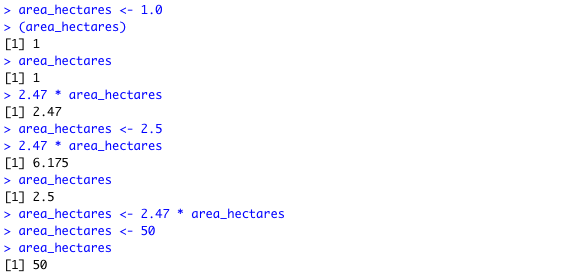
\includegraphics[width=\textwidth]{Images/RStudio_3.png}
\begin{itemize}
\item \textbf{SUCCESS} Added value to the object hectares
\item \textbf{ERROR} Current content at the end should have been 6.175, however it comes up as 50. 
\end{itemize}
Comments \\
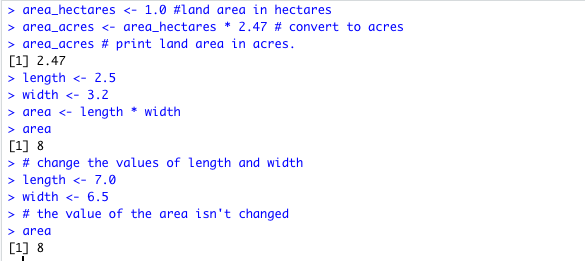
\includegraphics[width=\textwidth]{Images/RStudio_4.png}
\begin{itemize}
\item \textbf{SUCCESS} Created two variables length and width and assigned them values
\end{itemize}
Functions and Their Arguments \\
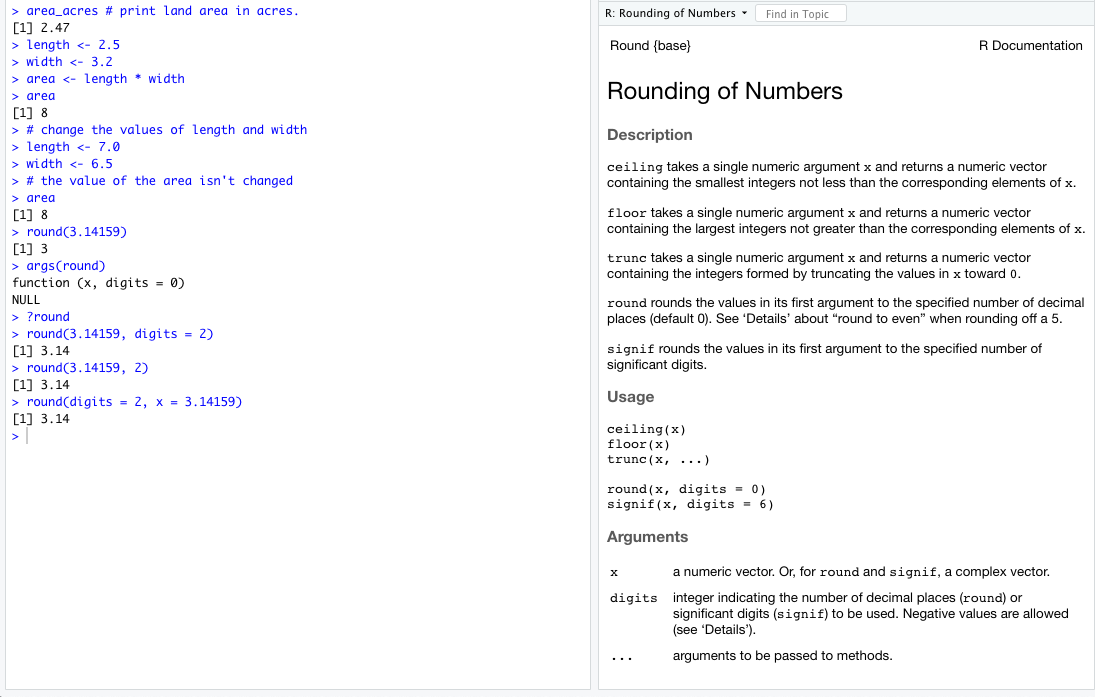
\includegraphics[width=\textwidth]{Images/RStudio_5.png}
\begin{itemize}
\item \textbf{SUCCESS} Command opened Rounding of Numbers in right help panel 
\end{itemize}
Vectors and Data Types \\

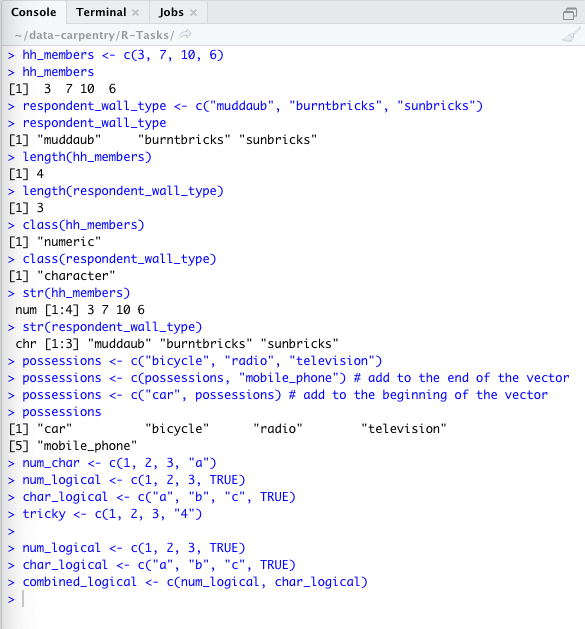
\includegraphics[width=\textwidth]{Images/RStudio_6.png}
\begin{itemize}
\item \textbf{SUCCESS} Assigned a series of values using the c() function
\item \textbf{SUCCESS} Inspected the content of a vector 
\item \textbf{SUCCESS} Function class() indicated type of element
\end{itemize}
Missing Data \\
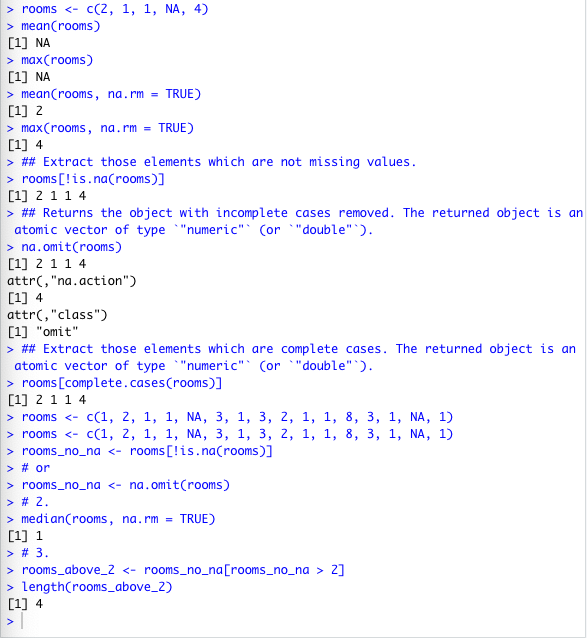
\includegraphics[width=\textwidth]{Images/RStudio_7.png} 
\begin{itemize}
\item \textbf{SUCCESS} Added argument to NA and calculated result whilst ignoring missing values
\item \textbf{SUCCESS} Created a new vector with the NAs removed
\end{itemize}

\subsection{Key Points}
Before We Start \\
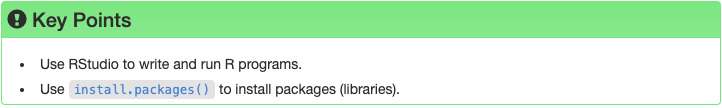
\includegraphics[width=\textwidth]{Images/RStudio_2.png} \\
Introduction to R \\
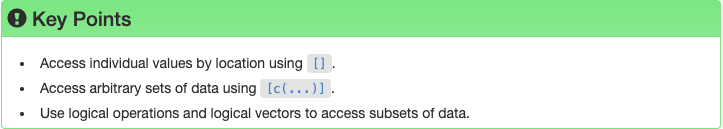
\includegraphics[width=\textwidth]{Images/RStudio_8.png} \\

\subsection{Final Thoughts}
\textbf{10:12PM} Brain is frazzled. Data carpentry is an overload of new language that I do not have time to take in or grasp meaningfully. Not with the amount of work we have for the rest of this unit, or at this time of semester. I think I would really enjoy this program and learning about it, however - it should be the whole semesters focus learning and understanding these programs. I'm unable to comprehend and focus because I need to be creating my own automation process. It is all too much. Feeling disheartened but will continue with the rest during the week. 


\section{22/10/2019}
\subsection{Thoughts/Intentions}
\textbf{3:17PM} Going to try smash out the rest of R for social scientists so I can get on with working through the POC. I am really nervous that I won't be have a final POC at the moment. I will screenshot images of my work in R and record success or errors like the journal entry above. Working on Starting with Data. \\
\textbf{4:21PM} Starting Introducing dplyr and tidyr

\subsection{Actions}
Presentation of the SAFI Data \\
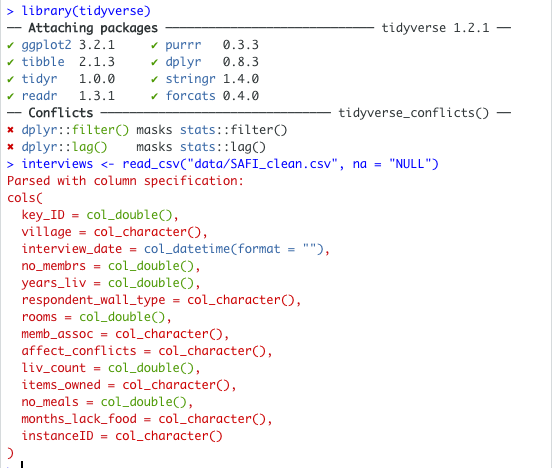
\includegraphics[width=\textwidth]{Images/RStudio_9.png}
\begin{itemize}
\item \textbf{SUCCESS} Loaded R's memory using read cvs function
\item \textbf{SUCCESS} Loaded the package with NULL included
\end{itemize}

Indexing and Subsetting Data Frames (Next page) \\
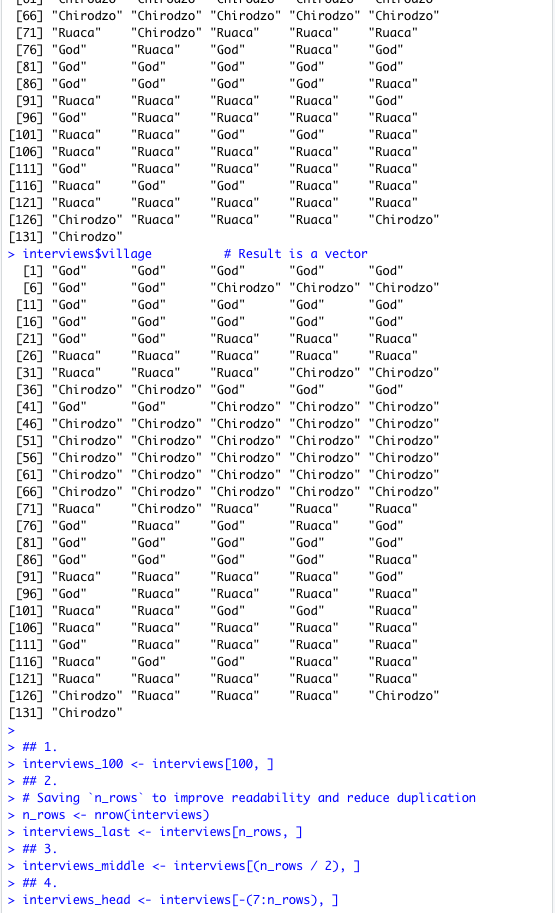
\includegraphics[width=\textwidth]{Images/RStudio_10.png}
\begin{itemize}
\item \textbf{SUCCESS} Extracted specific data 
\item \textbf{SUCCESS} Excluded indices of data frame with - sign
\item \textbf{ERROR} or \textbf{SUCCESS} Unsure if exercise was completed in final 10 lines (see above) as command in console did not produce a result
\end{itemize}

Factors \\
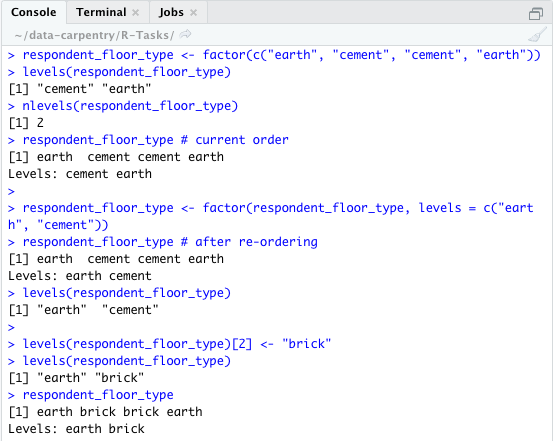
\includegraphics[width=\textwidth]{Images/RStudio_11.png}
\begin{itemize}
\item \textbf{SUCCESS} Reordered levels in respondent floor type vector
\item \textbf{SUCCESS} Re-coded cement to brick
\end{itemize}
\clearpage
Renaming Factors \\
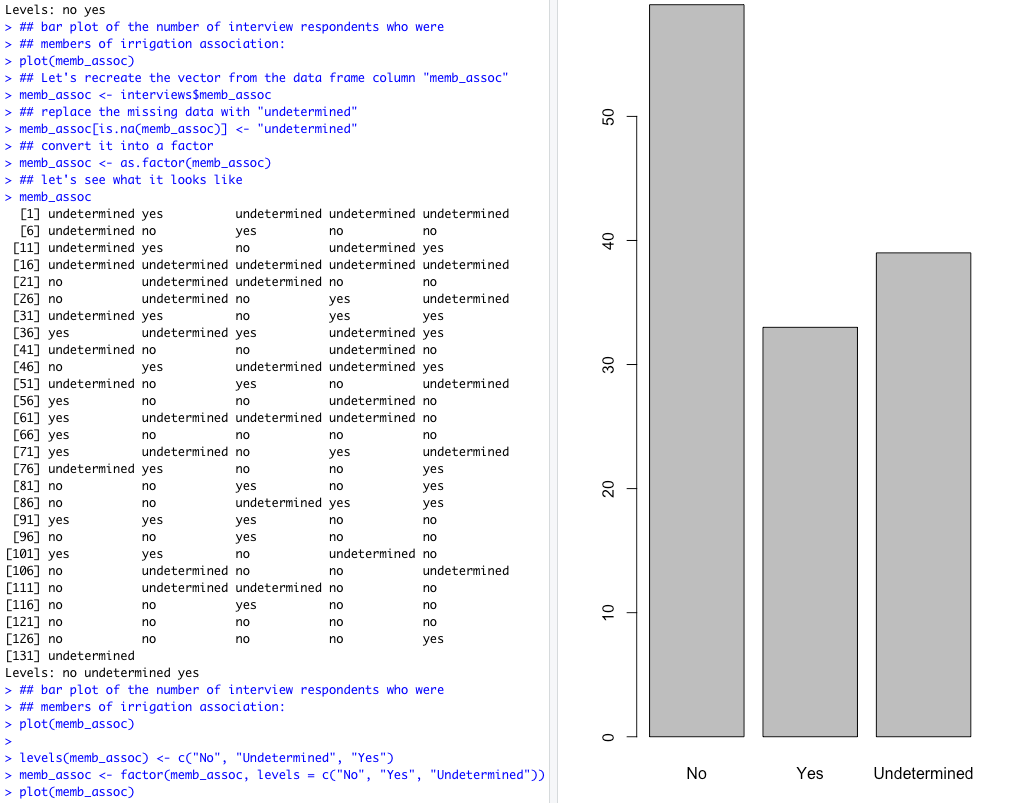
\includegraphics[width=\textwidth]{Images/RStudio_12.png}
\begin{itemize}
\item \textbf{SUCCESS} Renamed the levels of the factor to have uppercase 
\item \textbf{SUCCESS} Moved Undetermined bar to last
\end{itemize}

Learning dplyr and tidyr (Pipes - See next page) \\
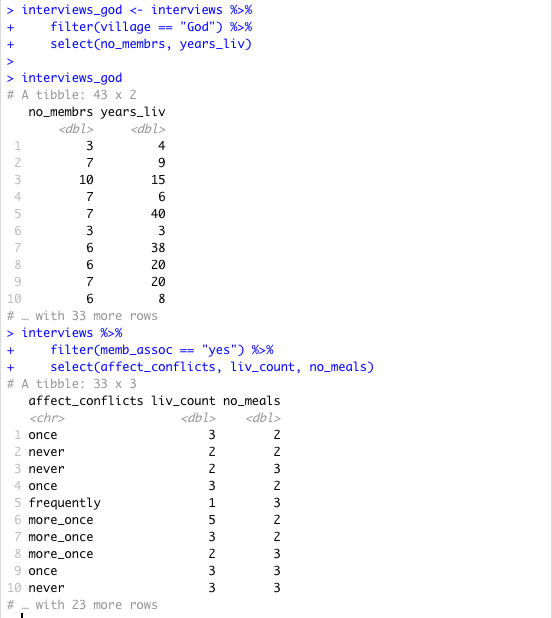
\includegraphics[width=\textwidth]{Images/RStudio_14.png} 
\begin{itemize}
\item \textbf{SUCCESS} Subsetted the interviews data through using pipes
\item \textbf{SUCCESS} Included interview filter mem assoc
\item \textbf{SUCCESS} Retained only columns affect conflicts, liv count and no meals by using select command
\end{itemize}
Mutate (See next page) \\
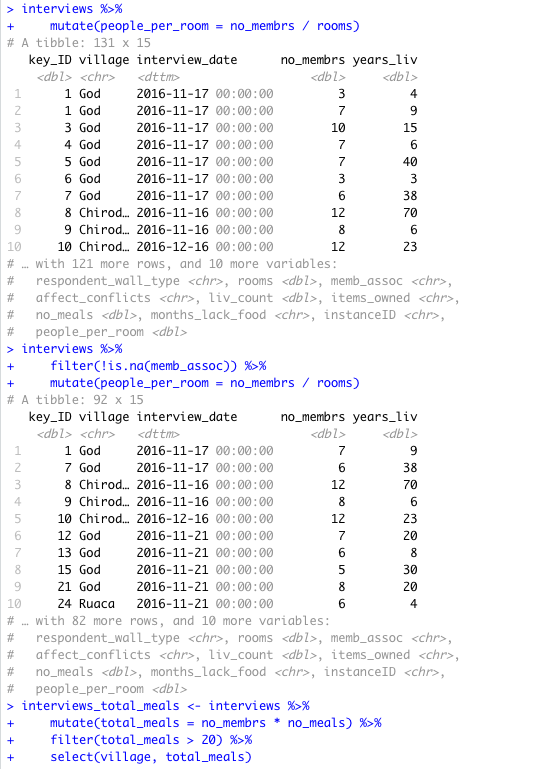
\includegraphics[width=\textwidth]{Images/RStudio_15.png}
\begin{itemize}
\item \textbf{SUCCESS} Found ratio of values in two columns using mutate command
\item \textbf{SUCCESS} Removed cases using filter in the chain
\item \textbf{ERROR} or \textbf{SUCCESS} Entered written command however no result appeared.
\end{itemize}
Counting (See next page) \\
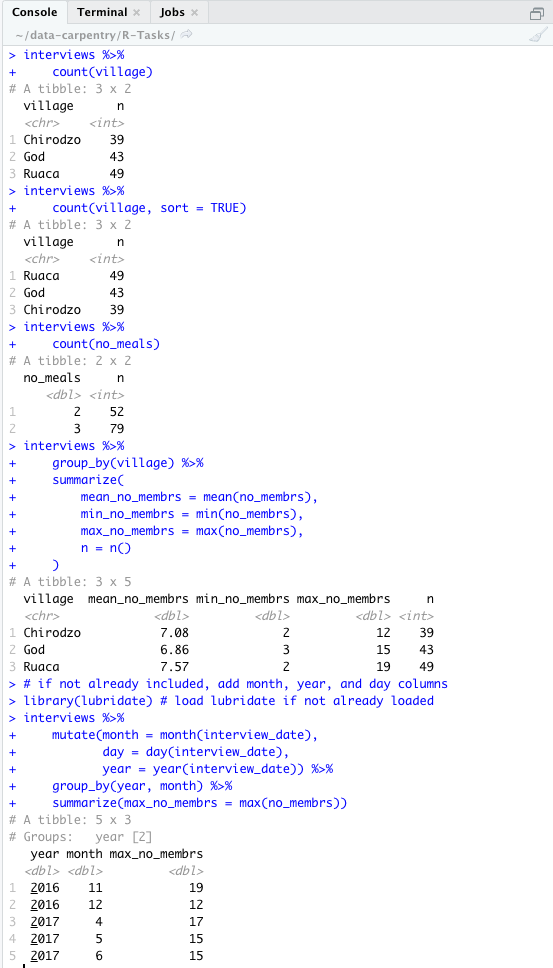
\includegraphics[width=\textwidth]{Images/RStudio_16.png}
\begin{itemize}
\item \textbf{SUCCESS} Used count to sort argument and result in decreasing order
\item \textbf{SUCCESS} Counted meals 
\item \textbf{SUCCESS} Summarised household members for each village
\item \textbf{SUCCESS} Found largest household 
\end{itemize}

Applying spread() to clean our data \\
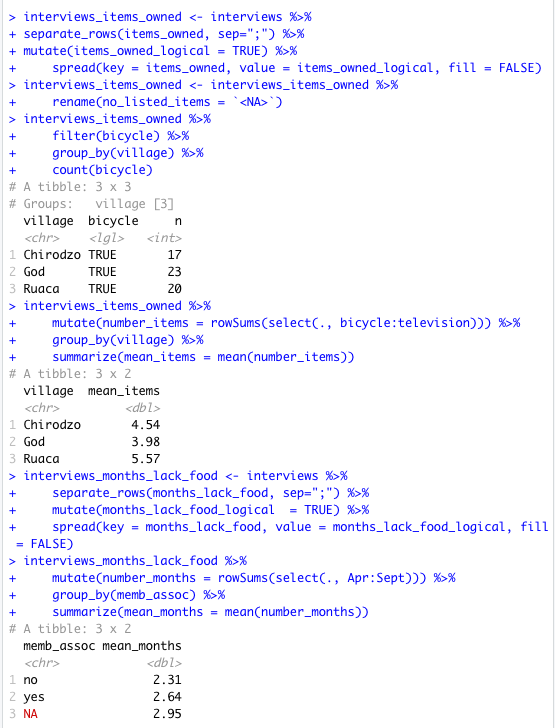
\includegraphics[width=\textwidth]{Images/RStudio_17.png}
\begin{itemize}
\item \textbf{SUCCESS} Created new data frame
\item \textbf{SUCCESS} Create one column for each month and true or false records
\item \textbf{SUCCESS} Identified months respondents didn't have food
\end{itemize}


\subsection{Key Points}
Starting With Data \\ 

\includegraphics[width=\textwidth]{Images/RStudio_13.png} \\
Learning dplyr and tidyr \\
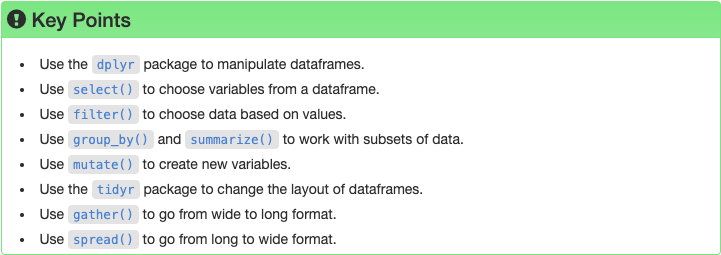
\includegraphics[width=\textwidth]{Images/RStudio_18.png} 

\subsection{Final Thoughts}
\textbf{4:50PM} Finished data carpentry, however I do not think any section in data carpentry has been retained throughout this semester. Entirely self-taught and skims so quickly over each section. If I was to truly gain something meaningful from DC I would need to spend weeks on each component yet our time is extremely limited. I unfortunately do not think there is value in teaching this in this limited format. 

\section{23/10/2019}
\subsection{Downloading Tools for POC}
One of the functions I have for this automation is backing up to an external drive or online storage system. Therefore I need to get Duplicati working.
\subsection{Thoughts/Intentions}
\textbf{9:46AM} Download and open Duplicati successfully

\subsection{Actions}
Download Duplicati
\begin{itemize}
\item Enter Duplicati website
\item Click on Download
\item Select macOS / OSX 2.0.4.23
\item Duplicati now downloading ontop laptop
\item Double click on dmg download
\item \textbf{ERROR} Same message received (see figure 13. below)
\end{itemize}

\begin{figure}[H]
    \centering
    
\includegraphics[width=\textwidth]{Images/Duplicati_warning.png}
    \caption{Duplicati Warning Prompt}
    \label{fig:my_label}
\end{figure}

\subsection{Final Thoughts}
\textbf{10:05AM} I've messaged Brian because I don't know how to get passed this. I also feel like I've hit a wall with the POC and really unsure how I'm meant to tie everything together. No idea where to start with a script. Going to try learn more about scripts and see if I can tie in or move any files into Tropy. \\
\textbf{10:09AM} Realised hes offline till Friday. Will try re-learning using shell script again whilst I wait for a response. MINDDDD IS IMPLODING BLAAHHHHHHH

\section{25/10/2019}
\subsection{POC TESTS: Export Photos and Shell}
Since I'm stuck on everything but automator I'm going to streamline the process to make it easier for when I'm able to write the shell script.
\subsection{Thoughts/Intention}
\textbf{10:30AM} Go through the automator process to simplify names in exported folder and photos \\
\textbf{10:35AM} Change eventual folder name from photos exports to tropy input \\
\textbf{11:30AM} After watching some tutorials and working with Unix I want to display command in shell that just worked to reach folder

\subsection{Actions}
\begin{itemize}
\item Run Export Photos shell script
\item Click results 
\item Remove add date section in action: "rename finder items: Make sequential
\item Run shell script
\item \textbf{SUCCESS} Photos are now more basic without dates, written as "ChanguField"
\end{itemize}
Rename Folder
\begin{itemize}
\item Add action "find finder items" 
\item Search organise photo
\item Select "all" of the following are true
\item Select date last modified
\item Add action rename finder items
\item Select replace text
\item Type in find bar: Photos Export 
\item Select in basename only and ignore case
\item Type in replace tropy input (underscore as the space inbetween)
\item Run shell script
\item \textbf{ERROR} Name does not change
\item Add action get selected finder items after "find finder items" action
\item Run shell script
\item \textbf{SUCCESS} Folder is renamed as tropy input (see figure below for screenshot of actions)
\end{itemize}

\begin{figure}[H]
    \centering
    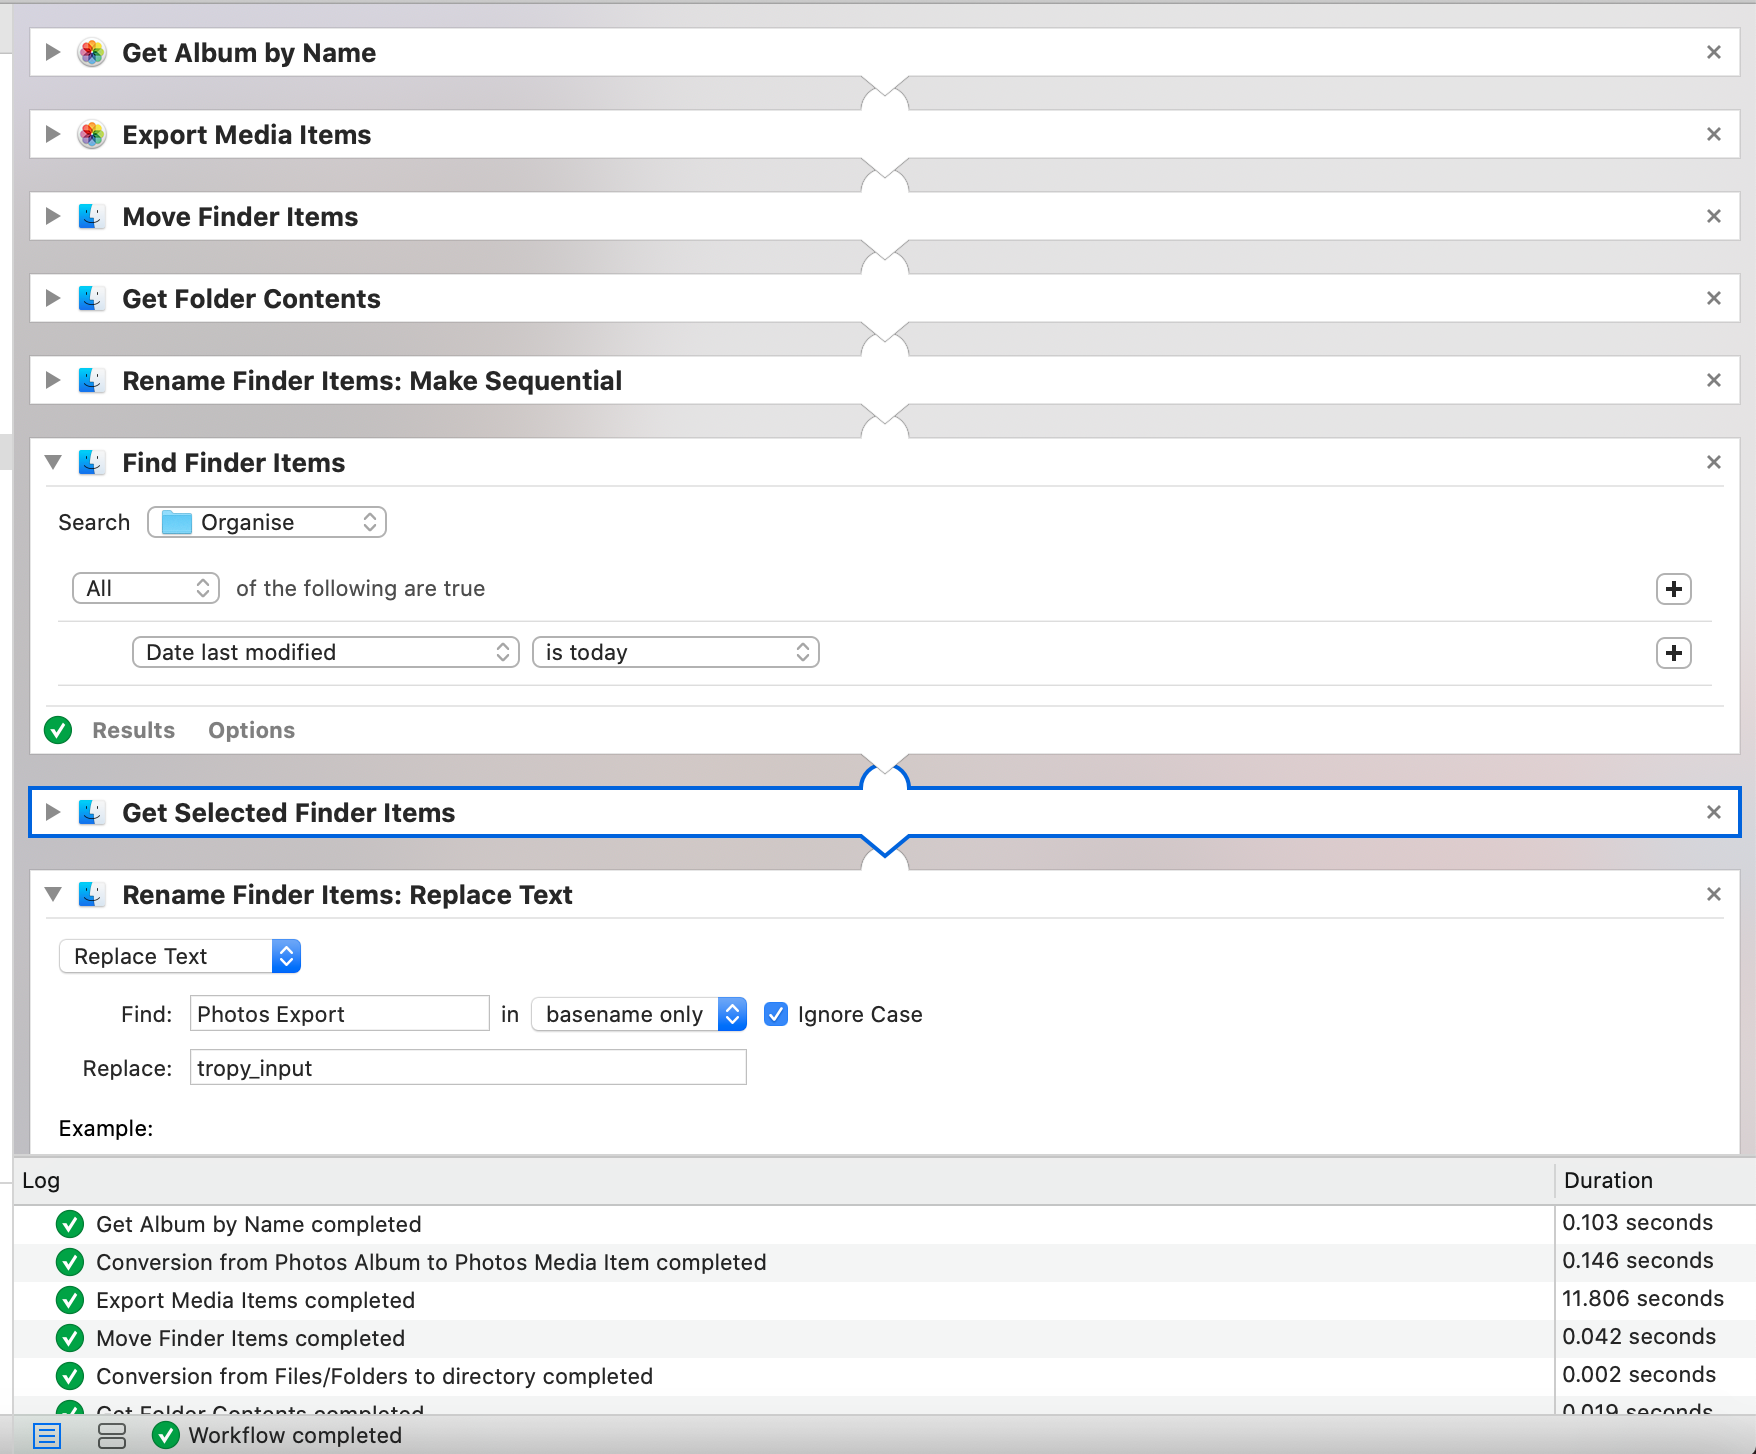
\includegraphics[width=\textwidth]{Images/Automator_5.png}
    \caption{New Actions in Automation}
    \label{fig:my_label}
\end{figure}

Unix Shell Command to Reach Tropy
\begin{itemize}
\item Command pwd 
\item Command cd desktop
\item Command cd organise

\begin{verbatim}
Command ls | grep_tropy input 
\end{verbatim}  
\item \textbf{SUCCESS} Tropy input folder is in shell (See figure 15 below)
\end{itemize}

\clearpage
\begin{figure}[H]
    \centering
    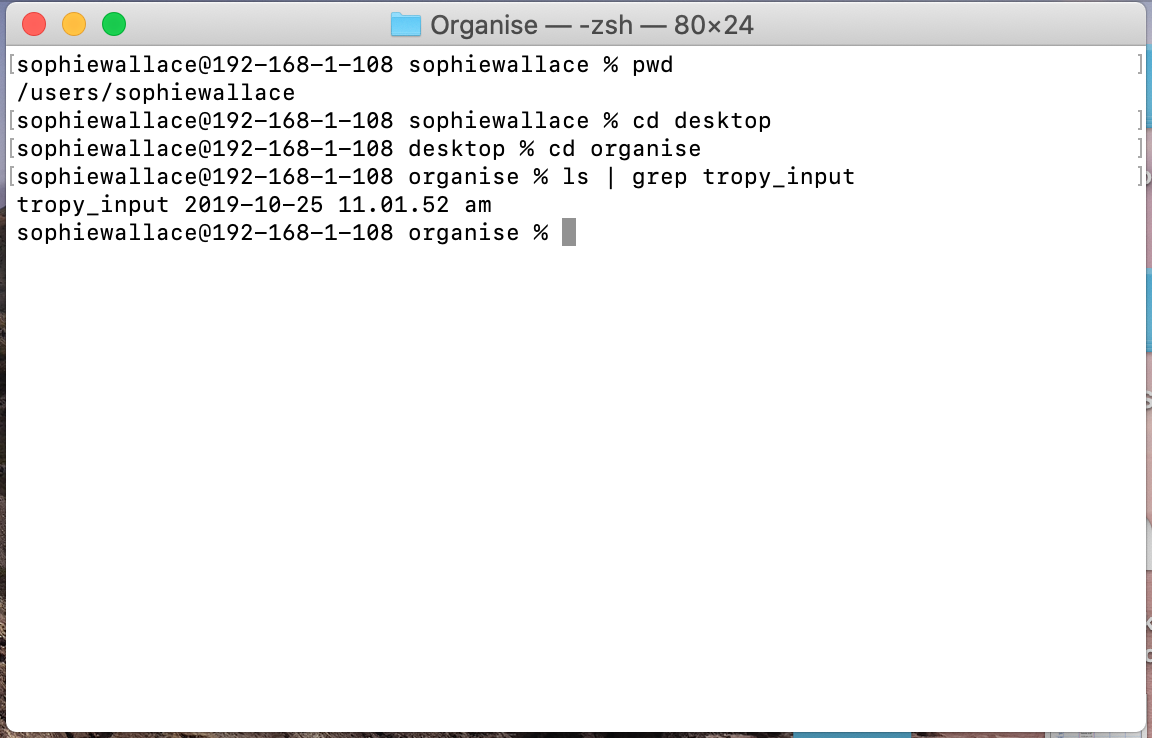
\includegraphics[width=\textwidth]{Images/Unix_1.png}
    \caption{Unix Commands to Reach Tropy Input Folder}
    \label{fig:my_label}
\end{figure}


\subsection{Final Thoughts}
\textbf{10:57AM} Progress is very minor, albeit more refined. Would love to be working with shell and/or duplicati and refining my overall POC rather than the only function I have working. \\
\textbf{11:30AM} At least I'm able to get to the point where I am seeing the folder I need to move into Tropy. Although this process will be slow I think I need to work like this to be able to understand what I'm doing - rather than just typing commands like data carpentry. I still need to figure out how to combine this code with exiftool, grab the template, put it into Tropy and run Duplicati... Seems impossible at the moment but staying optimistic.

\section{25/10/2019}
\subsection{POC Tests: Duplicati and Unix Shell Command}
Working with Kathryn I was able to successfully download Duplicati and work with an exiftool command to add metadata to an image.
\subsection{Thoughts/Intentions}
\textbf{1:48PM} Documenting exiftool command that adds metadata into image.

\subsection{Actions}
Unix Shell Command
\begin{figure}[H]
    \centering
    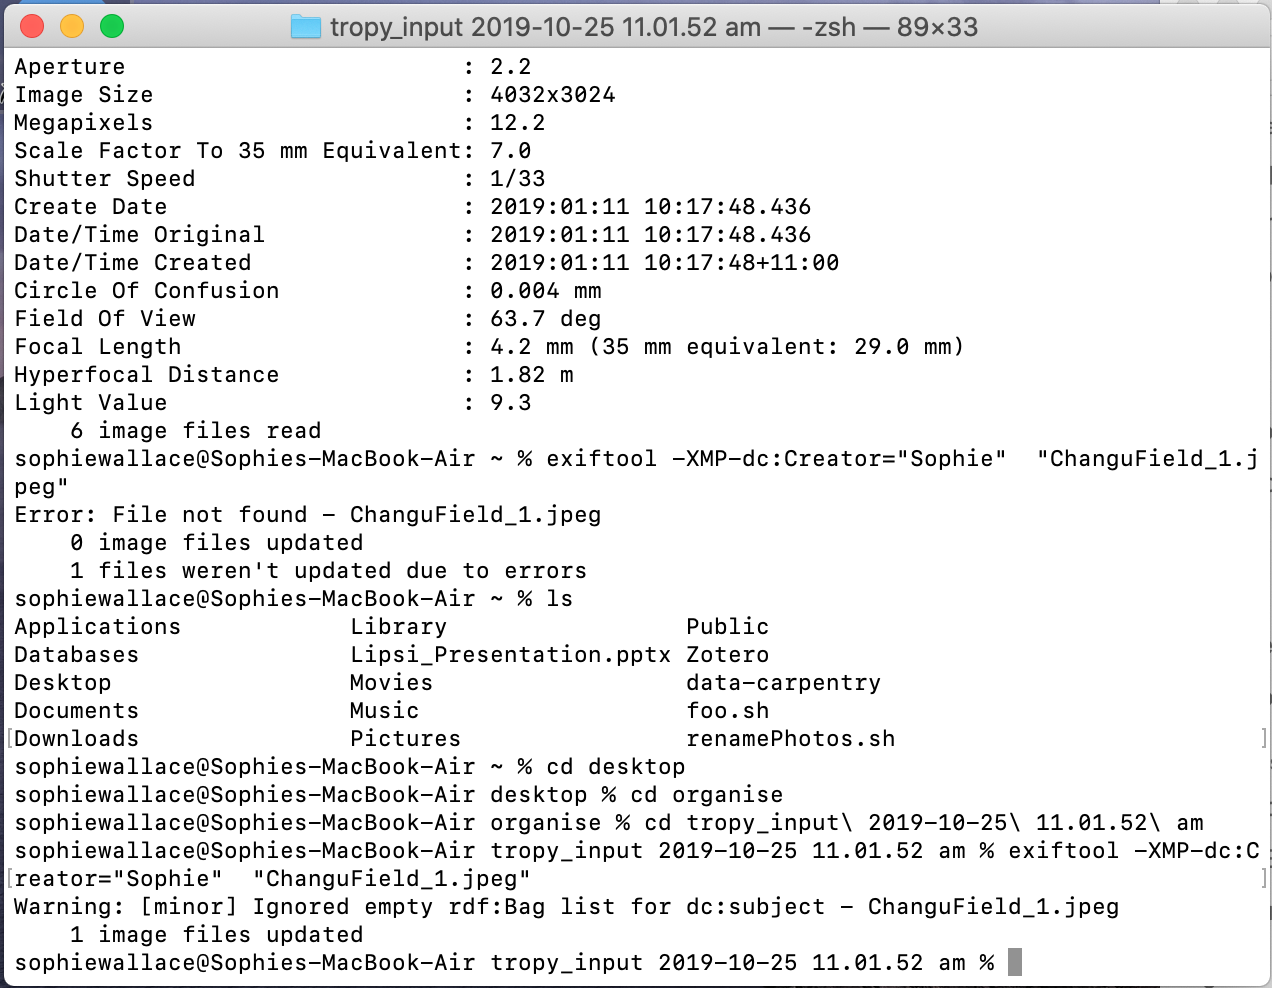
\includegraphics[width=\textwidth]{Images/Exiftool_3.png}
    \caption{ExifTool Command to Add Metadata Into Image}
    \label{fig:my_label}
\end{figure}

\textbf{Key Command Once Located in Image Folder}
\begin{verbatim}
exiftool -XMP-dc: Creator="Sophie" "ChanguField_1.jpeg"
\end{verbatim}

\subsection{Final Thoughts}
\textbf{6:30PM} Had to go to class so wasn't able to complete entry. I'm feeling a lot better talking to Kathryn and seeing the direction I can take. I also was reminded about for loops, which I will need to play around with a lot to get something working with exiftool. Have a lot of stuff to work on now so hopefully I can get somewhere.  \\
\textbf{TIP:} Use tab key in command shell to fill out the additional writing after basename i.e. tropy input "tab"

\section{25/10/2019}
\subsection{POC TEST: Bash Script}
After playing around with bash script I want to be able to write what I have down so there is a clear example of the steps I have so far.
\subsection{Thoughts/Intention}
\textbf{7:49PM} Write shell script so far. This is with the folder beginning in home directory \\
\textbf{8:32PM} Finding the location in photos is a current issue I'm having. Entered mac default photos app to look at geotag "places" in photo. Photos I am currently using are not located - so trying different photos and uploading into exiftool.

\subsection{Actions}
Bash Script
\begin{verbatim}
cd POC_Contents
cd Organise
cd Tropy_Input"tab"
exiftool ChanguField *
\end{verbatim}
\textbf{SUCCESS} Inside tropy photos folder and exiftool has opened up each photo \\
Photo Location
\begin{itemize}
\item Place already geotagged photos in export folder
\item Open Export Automation workflow in automator
\item Run script
\item Open shell terminal
\item type exiftool and drag in photo
\item \textbf{ERROR} Still no GPS or location in exif metadata
\end{itemize}


\subsection{Final Thoughts}
\textbf{8:36PM} Spent a solid few hours trying to look through for loops and shell scripts, don't feel like I've found a clearer direction. The location in the photo is annoying me because its obviously there for apple programs to see so I'm not sure why exif or Tropy are not picking this up. Will figure out down the track. Good luck to future Sophie. 

\section{31/10/2019}
\subsection{POC TEST: Bash Script}
Currently testing out how to use exif tool, how to iterate commands and whether it works in mac automator. I have been working on this for a few hours already, however I wanted to document some of the progress and errors.
\subsection{Thoughts/Intention}
\textbf{11:25AM} Write new bash script that works for now. This relies on whether mac automator successfully changes the name of the folder to tropy input. \\
\textbf{1:14PM} After trying to figure out everythign over the past few hours, I'm going to just copy and paste a screenshot of my current progress and issues. See figure 17 after final thoughts.

\subsection{Actions}
Updated Bash Script
\begin{verbatim}
cd POC_Contents
cd tropy_input*
exiftool -Creator="Sophie Wallace" *.jpeg
\end{verbatim}

\subsection{Final Thoughts}
\textbf{1:21PM} I've been working on this since 7:30am and still feel that I have so many roadblocks that are preventing me from moving forward. I have been able to apply metadata to multiple images in exiftool so that is one basic function complete that took hours. The current shell script I have is only three lines using exiftool. Once I can copy images into tropy hopefully that will add more - however I do feel like mac automator has done the majority of work. Unsure how  this will impact my mark. 


\begin{figure}[H]
    \centering
    \includegraphics[width=\textwidth]{Images/Progress.png}
    \caption{Current Progress}
    \label{fig:my_label}
\end{figure}

\section{07/11/12}
\subsection{POC Tests: Running on a different system}
After consultation with Brian, a lot of my issues have been solved on this computer. However, I still need to see if its replicable on another laptop. I'm now on another laptop to test if I can follow the instructions in my Github repository ReadMe and successfully download and run everything.
\subsection{Thoughts/Intentions}
\textbf{3:07PM} Go through requirements section in ReadMe \\
\textbf{3:58PM} Now going to test installation \\
\textbf{4:07PM} Repository is cloned and images are in a new folder in Mac Photos called Export. Now testing Workflow

\subsection{Actions}
Tropy
\begin{itemize}
\item Click tropy download link
\item \textbf{SUCCESS} Tropy begins downloading
\item Click show tropy in finder
\item Double click Tropy.dmg file
\item \textbf{SUCCESS} Tropy is downloaded onto system
\end{itemize}

ExifTool
\begin{itemize}
\item Click ExifTool link
\item \textbf{SUCCESS} ExifTool begins to download
\item Click on Exiftool download
\item Double click on exiftool package in prompt
\item \textbf{ERROR} ExifTool doesn't open due to being from an unidentified server
\item Right click on exiftool package and open with terminal
\item Double click on exiftool package
\item \textbf{SUCCESS} ExifTool installer appears
\item Go through installation process
\item \textbf{SUCCESS} Exiftool is now installed
\end{itemize}

Duplicati
\begin{itemize}
\item Click on Duplicati link 
\item \textbf{SUCCESS} Duplicati downloads
\item Click on duplicati download
\item \textbf{ERROR} The following disk image couldn't be opened
\item Show Duplicati download in finder
\item right click on Duplicati and click open
\item \textbf{ERROR} Same message as above
\item Find Duplicati website
\item Download directly from websitee
\item Click open once downloaded
\item \textbf{SUCCESS} Duplicati downloaded into applications
\end{itemize}

GitHub Desktop
\begin{itemize}
\item Click on GitHub Desktop link
\item \textbf{SUCCESS} GitHub desktop downloads
\item Double click on github desktop download
\item \textbf{SUCCESS} github desktop is downloaded
\end{itemize}

Cloning repository
\begin{itemize}
\item Open POC Contents repository
\item \textbf{SUCCESS} POC Contents are now in system
\end{itemize}

Testing Workflow
\begin{itemize}
\item Open POC Automator File
\item \textbf{ERROR} The action "Get Album by Name" could not be loaded because it could not be located
\item \textbf{ERROR} The action "Export Medeia items" could not be loaded because it could not be located "Try reinstalling this action
\item Reinstall actions
\item Run Automation test
\item \textbf{ERROR} Location not detected
\end{itemize}

\subsection{Final Thoughts}
\textbf{4:31PM} All downloads worked well, with some tweaking. I might need to just include that in the limitations/predetermined issues. I need to change a lot of the locations in the workflow automation to make it successful on another computer, which I will do now.

\section{07/11/2019}
\subsection{POC Tests: Progress}
After fixing some of the ExifTool script with Brian's help I thought I should document the updates and changes in this journal. It is hard to maintain this journal when there are so many elements to record and a lot of progress happening during consultation hours.
\subsection{Thoughts/Intentions}
\textbf{6:22PM} Documenting updates and progress that has occurred over the past week in this POC. 

\subsection{Updates}
\begin{itemize}
\item \textbf{Tropy does not work with the command line:} this shifted my expectations for the final product. Photos would not be able to be moved into Tropy through a shell script. This was both gratifying and disheartening, because although I knew I had spent a lot of time trying to work with this - I was glad to know that it was not an error of mine that prohibited this from working. However, that meant changing the approach.
\item \textbf{Tested different tools:} the first approach was to try a different tool over Tropy. This tool was called darktable. After downloading and opening the program, its interface and functions prioritised photo editing over metadata management. Tropy remained the most appropriate program for this eventual POC.
\item \textbf{Changed approach to Automator:} now that photos cannot be imported to Tropy via script, a more streamlined process in automator was created. This included implementing the action "Watch Me Do" at the end. This allows for the final action of the demonstration to display Tropy and the folder with updated photos next to eachother in a tiled window. This looks effective, however is not replicable on other computers.
\item \textbf{Updated ExifTool Script:} the exiftool script I created worked fine, however it only added the creator. Working with Brian we were able to add the original date of the photo, rename the image and create a prompt to ask for location. This allows for arbitrary metadata to be added to the image. This is a significant improvement and enables the workflow to rely less on haphazard actions.
\item \textbf{Added License:} I also added a license in my GitHub repository to professionalise the software package. 
\item \textbf{GitHub README:} I have started writing the background, outline, requirements, installation, testing workflow, limitations and further information sections in my README for the POC implementation. 
\end{itemize}

\subsection{Final Thoughts}
\textbf{6:40PM} I am really happy with how much progress has occurred over this past week. I feel like I have an actual POC to submit on Sunday and it is something I am proud of and feel I will use in the future. There are still some requirements I need to sort out, mainly how to instruct the user to implement Duplicati and creating criteria for Quality Assurance . Other than that I am pretty happy with how it has turned out. Hopefully, this will be enough for a substantial outcome. 

\section{08/11/2019}
\subsection{Final POC Components}
I want to include the final POC components that work in a separate system to display how it has evolved over time. 
\subsection{Thoughts/Intentions}
\textbf{10:38AM} Show final Automator workflow \\
\textbf{11:02AM} Show final ExifTool script \\
\textbf{11:20AM} Show (almost) final GitHub Repository

\subsection{Automator Workflow}
The final workflow automation includes nine actions that work chronologically. \\
The first four actions automate moving the images from the default Mac Photo application onto Desktop. This is the initial step to prepare them for added metadata and moving into Tropy. These set up actions are in Figure 18 below:

\begin{figure}[H]
    \centering
    \includegraphics[width=\textwidth]{Images/Final_Automation1.png}
    \caption{Export Actions}
    \label{fig:my_label}
\end{figure}

The next step is adding metadata. The first two actions find the folder and rename it to tropy input with the asterisks including the current date and time when they were exported. Thereafter, a prompt appears asking for text to embed the image with arbitary metadata. This prompt asks "What is the geo-location of these images?". A shell script then runs a code to embed the image with metadata including the author i.e. Sophie Wallace, renaming the images to Nepal and original creation date and time, and prioritises the date of the image to display the creation date and time when in Tropy. The actions for adding metadata are seen below in Figure 19. 

\begin{figure}[H]
    \centering
    \includegraphics[width=\textwidth]{Images/Final_Automation2.png}
    \caption{Metadata Actions}
    \label{fig:my_label}
\end{figure}

Lastly, the automator workflow launches Tropy for the photos to be manually dragged in. Due to the command line not working with Tropy, this was the most appropriate way to input photos. The final outcome of the images in Tropy can be seen in Figure 20 below. The final workflow displaying all the actions can be seen in Figure 21 below.

\begin{figure}[H]
    \centering
    \includegraphics[width=\textwidth]{Images/Final_Tropy1.png}
    \caption{Final Images in Tropy}
    \label{fig:my_label}
\end{figure}

\begin{figure}[H]
    \centering
    \includegraphics[width=\textwidth]{Images/Final_Automation3.png}
    \caption{Complete Automator Workflow}
    \label{fig:my_label}
\end{figure}

\subsection{ExifTool Script}
This script started with only adding author metadata to one image and was external to the Automator workflow. With the help of Brian, we were able to include this script inside the workflow and add more metadata such as location, original date and renaming the images. Renaming images was important due to the unreliable nature of the automator renaming action. Now the script should be consistent. There are two sections of this script. See Figure 22 for the separate script. See Figure 23 for the script inside Automator.

\begin{figure}[H]
    \centering
    \includegraphics[width=\textwidth]{Images/ExifTool_Final1.png}
    \caption{Separate ExifTool Script}
    \label{fig:my_label}
\end{figure}

\begin{figure}[H]
    \centering
    \includegraphics[width=\textwidth]{Images/ExifTool_Final2.png}
    \caption{Automator Shell Script}
    \label{fig:my_label}
\end{figure}

\subsection{GitHub Repository}
The GitHub Repository now includes almost all components needed for the POC demonstration. The quality assurance criteria needs to still be added. This will be included tomorrow. See Figure 24 for the almost complete GitHub Repository. 

\begin{figure}[H]
    \centering
    \includegraphics[width=\textwidth]{Images/GitHub_Final1.png}
    \caption{GitHub Repository}
    \label{fig:my_label}
\end{figure}

\subsection{Final Thoughts}
\textbf{11:28AM} Again, I'm happy with the final product. The fact that all of the automation is inside Automator is great because I thoguht I would need to write another script that would have to be run separately to automator. This adds to the streamlined process. This demonstration discussed above is a more simplified version of the one I have on my computer however I'm pleased with its applicability. Hopefully it works on the the demonstrators computer! As mentioned above, I still have to work with Duplicati, the PICO Presentation and the Acceptance Criteria. However, as this journal is handed in today by 2PM I wanted to make sure the final product was documented. 




\end{document}
